\documentclass[a4paper]{article}

\usepackage{
  amsmath, 
  amsfonts, 
  amssymb, 
  amsthm, 
  mathtools,
  geometry,
  fontspec,
  microtype,
  listings,
  minted,
  graphicx,
  xcolor,
  polyglossia,
  hyperref,
  float,
  pdfpages
}
\usepackage[14pt]{extsizes}
\usepackage[acronym, xindy, toc]{glossaries}
\usepackage[
  backend=biber,
  bibencoding=utf8,
  bibstyle=gost-numeric,
  language=autobib,
  autolang=other,
  clearlang=true,
]{biblatex}
\usepackage[center]{titlesec}

\addbibresource[datatype=bibtex]{references.bib}

\linespread{1.3} % Как ни странно соответствует полуторному интервалу https://ru.wikibooks.org/wiki/LaTeX/Форматирование_текста
\setmainfont[Ligatures=TeX]{Times New Roman}
\newfontfamily\listingsfont[Scale=.8]{Menlo}
\newfontfamily{\cyrillicfonttt}{Menlo}

\geometry{ 
  left=30mm, 
  top=20mm, 
  right=15mm, 
  bottom=20mm, 
  footskip=10mm, 
  nohead=true 
}
\setlength\parindent{1.25cm}
\graphicspath{ {./images/} }
\setminted{ fontsize=\footnotesize }

\urlstyle{same}

% Не очень хорошо
\sloppy

\setmainlanguage{russian}
\setdefaultlanguage{russian}
\setotherlanguages{english}

\definecolor{codegreen}{rgb}{0,0.6,0}
\definecolor{codegray}{rgb}{0.5,0.5,0.5}
\definecolor{codepurple}{rgb}{0.58,0,0.82}

\lstdefinelanguage{typescript}{
  keywords={typeof, new, true, false, catch, function, return, null, catch, switch, var, const, let, if, in, while, do, else, case, break, type},
  keywordstyle=\color{blue},
  ndkeywords={class, export, boolean, string, number, throw, implements, import, from, this},
  ndkeywordstyle=\color{magenta},
  identifierstyle=\color{black},
  sensitive=false,
  comment=[l]{//},
  morecomment=[s]{/*}{*/},
  commentstyle=\color{codegreen},
  stringstyle=\color{codepurple},
  morestring=[b]',
  morestring=[b]"
}

\lstdefinelanguage{vue}{
  keywords={typeof, new, true, false, catch, function, return, null, catch, switch, var, const, let, if, in, while, do, else, case, break, type, v-if, v-else, v-for, style, script, v-slot},
  keywordstyle=\color{blue},
  ndkeywords={class, export, boolean, string, number, throw, implements, import, from, this, template, div, svg, v-app-bar, v-btn, v-main, v-text-field, v-checkbox, v-card, v-card-actions, v-dialog, v-switch, v-icon, v-list, v-hover, v-list-item, span, v-divider, v-app, component},
  ndkeywordstyle=\color{magenta},
  identifierstyle=\color{black},
  sensitive=false,
  comment=[l]{//},
  morecomment=[s]{/*}{*/},
  commentstyle=\color{codegreen},
  stringstyle=\color{codepurple},
  morestring=[b]',
  morestring=[b]",
  alsoletter=-,
}

\lstdefinelanguage{scss}{
  keywords={@import, body},
  keywordstyle=\color{codegreen},
  identifierstyle=\color{black},
  stringstyle=\color{codepurple},
  sensitive=false,
  comment=[l]{//},
  morecomment=[s]{/*}{*/},
  morestring=[b]',
  morestring=[b]"
}

\lstdefinestyle{mystyle}{
  basicstyle=\linespread{0.8}\listingsfont,
  numberstyle=\linespread{0.8}\listingsfont\color{codegray},
  breakatwhitespace=false,
  breaklines=true,
  captionpos=b,
  keepspaces=true,
  numbers=left,
  numbersep=10pt,
  showspaces=false,
  showstringspaces=false,
  showtabs=false,
  tabsize=2,
  escapeinside={\%*}{*)},
}

\lstset{style=mystyle}

\renewcommand\lstlistingname{Листинг}


\makenoidxglossaries

\newglossaryentry{реактивность}{
  name=реактивность,
  description={способность фрагмента кода автоматически обновляться или перерисовываться (реагировать) в ответ на изменения в данных, к которым он привязан}
}
\newglossaryentry{транспиляция}{
  name=транспиляция,
  description={преобразование программы, написанной на одном языке программирования в качестве исходных данных, в эквивалентный код другой версии этого языка или в другой язык программирования того же уровня абстракции}
}
\newglossaryentry{вид}{
  name=вид,
  description={состояние приложения которое определяется набором и расположением представленных элементов графического интерфейса}
}
\newglossaryentry{модальное окно}{
  name={модальное окно},
  description={окно, которое блокирует работу пользователя, но оставляет главный экран видимым вместе с модальным окном. Пользователи должны взаимодействовать с модальным окном, прежде чем смогут вернуться в родительское приложение}
}
\newglossaryentry{фреймворк}{
  name=фреймворк,
  description={программное обеспечение, которое описывает правила построения архитектуры приложения, задавая на начальном этапе разработки поведение по умолчанию --- <<каркас>>, который нужно расширять и изменять, согласно некоторым требованиям}
}

\newacronym{волс}{ВОЛС}{волоконно-оптическая линия связи}
\newacronym{ор}{ОР}{оптический рефлектометр во временной области}
\newacronym{мор}{МОР}{метод обратного рассеяния}
\newacronym{сор}{СОР}{сигнал обратного рассеяния}
\newacronym{фпу}{ФПУ}{фотоприемное устройство}
\newacronym{лвт}{ЛВТ}{линейный волоконный тракт}
\newacronym{ов}{ОВ}{оптическое волокно}
\newacronym{teo}{TEO}{энергетический оператор Тигера (Teager energy operator)}
\newacronym{otdr}{OTDR}{Optical time domain reflectometer (оптический рефлектометр)}
\newacronym{по}{ПО}{программное обеспечение}


\begin{document}

% Титульный лист

\includepdf[pages=-]{title.pdf}

\section*{РЕФЕРАТ}
\thispagestyle{empty}

В выпускной квалификационной работе рассматривается тема «Методы и программное обеспечение для хранения и обработки результатов измерения оптических рефлектометров».

Выпускная квалификационная работа содержит: 78 страниц, 25 рисунков, 19 приложений.

В первом разделе приведен обзор предметной области и существующих решений.

Во втором разделе сформулированы требования к приложению и приведены детали технической реализации.

В третьем разделе продемонстрирована работа приложения.

ОПТИЧЕСКИЕ РЕФЛЕКТОМЕТРЫ, РЕФЛЕКТОМЕТРИЯ, ВОЛОКОННО-ОПТИЧЕСКИЕ ЛИНИИ СВЯЗИ, АНАЛИЗ ДАННЫХ, ХРАНЕНИЕ ДАННЫХ

Методы проведения работы: анализ литературы и публикаций, разработка компьютерной программы с использованием специализированной среды разработки.

Результаты работы и новизна: создан инструмент для просмотра результатов измерения рефлектометра, который позволяет интерпретировать события на линии, сохранять, организовывать и редактировать результаты измерений.

Области применения результатов: волоконно-оптические линии связи.

\newpage
\renewcommand{\contentsname}{СОДЕРЖАНИЕ}
\tableofcontents
\addtocontents{toc}{\protect\thispagestyle{empty}}
% Выключаем нумерацию страниц
\pagenumbering{gobble}

\newpage
\thispagestyle{empty}
% Тут сокращения и термины
\printnoidxglossary[
  title={ПЕРЕЧЕНЬ СОКРАЩЕНИЙ И ОБОЗНАЧЕНИЙ},
  type=\acronymtype
]

\newpage
\thispagestyle{empty}
\printnoidxglossary[
  title={СПИСОК ТЕРМИНОВ}
]

\newpage
% Включаем нумерацию страниц
\pagenumbering{arabic}
\setcounter{page}{12}
\section*{ВВЕДЕНИЕ}
\addcontentsline{toc}{section}{ВВЕДЕНИЕ}

% Во введении обосновывается актуальность темы, степень разработанности темы, указываются цель, задачи, объект и предмет исследования, используемые методы исследования и расчетов, определяется структура работы. Здесь также отражается теоретическая и практическая значимость работы. Объем введения ВКР бакалавра или специалиста составляет, как правило, 2-3 страницы.

Оптические рефлектометры широко используются в современных сетях связи для диагностики и обслуживания оптических кабелей. Они позволяют определять расстояние до места повреждения кабеля, а также определять потери сигнала на участках линии связи. Однако, эффективное использование оптических рефлектометров требует не только умения считывать и анализировать полученные результаты, но и специального программного обеспечения для их обработки и хранения.

Цель данной дипломной работы заключается в изучении методов и программного обеспечения для хранения и обработки результатов измерений оптических рефлектометров. В работе рассматриваются существующие методы и подходы к обработке и анализу данных, а также предлагаются новые подходы и методы для повышения эффективности использования оптических рефлектометров. Особое внимание уделено разработке и реализации программного обеспечения для автоматической обработки результатов измерений оптических рефлектометров.

Результаты данной работы могут быть использованы в сфере телекоммуникаций для повышения эффективности и надежности сетей связи. Также, разработанные методы и программное обеспечение могут быть применены в других областях, связанных с оптическими измерениями и анализом данных.

Тема <<Методы и программное обеспечение для хранения и обработки результатов измерения оптических рефлектометров>> является актуальной в настоящее время, так как использование оптических рефлектометров для диагностики и обслуживания оптических кабелей является неотъемлемой частью современных сетей связи. Оптические кабели используются для передачи большого объема данных, и их надежность является критически важной для функционирования сетей связи.

Однако, для эффективного использования оптических рефлектометров необходимо не только умение считывать и анализировать полученные результаты, но и специальное программное обеспечение для их обработки и хранения. Существующие методы и подходы к обработке и анализу данных могут быть улучшены и дополнены новыми подходами и методами, что позволит повысить эффективность использования оптических рефлектометров и обеспечить более надежную работу сетей связи.

Разработка новых методов и программного обеспечения для хранения и обработки результатов измерений оптических рефлектометров является важной задачей, которая позволит повысить качество и надежность работы сетей связи, улучшить диагностику и обслуживание оптических кабелей, а также снизить затраты на их обслуживание и ремонт. 
%В этом контексте, данная тема является актуальной и востребованной в научном и практическом плане.

\newpage
\section{ОБЗОР ПРЕДМЕТНОЙ ОБЛАСТИ}

%Обзор состояния рассматриваемого в ВКР вопроса на основании изучения литературных источников.

Наиболее универсальным прибором для измерений параметров волоконно-оптических линий связи (\acrshort{волс}) является оптический рефлектометр во временной области (\acrshort{ор}), работа которого основана на методе обратного рассеяния (\acrshort{мор}).

Рассеяние света происходит на флуктуациях показателя преломления кварцевого стекла, застывших при вытяжке волокна. Размер этих неоднородностей (релеевских центров) мал по сравнению с длиной волны и свет на них рассеивается во все стороны, в том числе и назад в моду волокна (рис. \ref{ris:obr_rass}).

\begin{figure}[h]
  \center{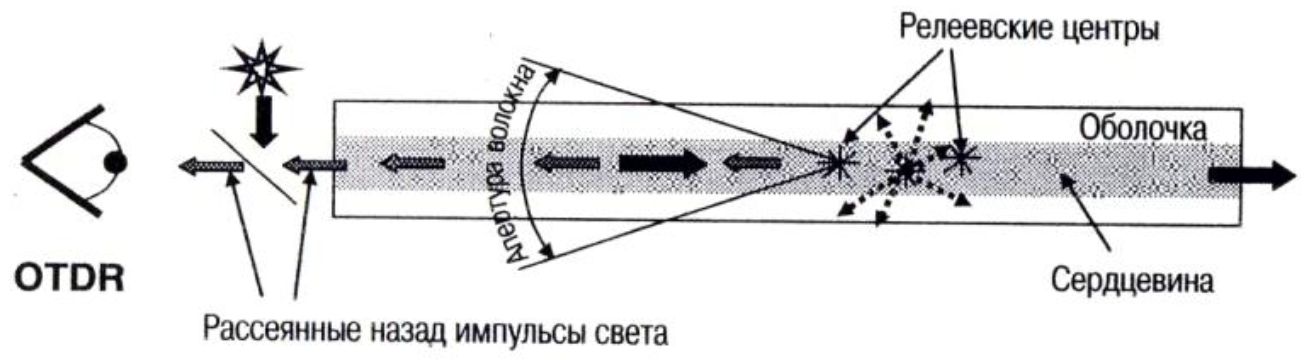
\includegraphics[width=\linewidth]{obr_rass}}
  \caption{В \acrshort{ор} приходят импульсы света рассеянные назад в моду волокна}
  \label{ris:obr_rass}
\end{figure}

Релеевские центры распределены однородно вдоль волокна, и в рассеянной на них волне содержится информация обо всех параметрах линии, влияющих на поглощение света. Именно за счет детектирования рассеянного излучения удается обнаруживать неотражающие (поглощающие) неоднородности в волокне. Например, по сигналу обратного релеевского рассеяния света можно измерить распределение потерь в строительных длинах оптических кабелей и потери в сростках волокон.

\acrshort{мор} основан на введении в \acrshort{ов} импульсного оптического излучения и последующем анализе сигнала обратного рассеяния (\acrshort{сор}), который возвращается на фотоприемное устройство (\acrshort{фпу}). В результате математической обработки \acrshort{сор} на экране \acrshort{ор} формируется изображение, называемое рефлектограммой и представляющее собой зависимость уровня \acrshort{сор} от расстояния вдоль линейного волоконного тракта~\cite{bogdanova:reflectometria}.

Угол наклона участков рефлектограммы между пиками характеризует погонное затухание по длине кабеля. Если в сегменте везде используется волокно одного и того же типа и качества, все участки рефлектограммы, снятой на одной длине волны, должны иметь одинаковый наклон.

\subsection{Устройство рефлектометра}

В большинстве моделей \acrshort{ор} используется модульная конструкция (рис.~\ref{ris:otdr_schematic}). Она содержит базовый модуль и несколько сменных оптических модулей. Базовый модуль представляет собой персональный компьютер, приспособленный для обработки сигнала и вывода его на дисплей. Оптический модуль включает в себя лазерный диод, фотоприемник, оптический ответвитель и оптический разъем. Стоимость оптического модуля зависит от величины его динамического диапазона и может в несколько раз превышать стоимость базового модуля. Модульная конструкция \acrshort{ор} позволяет потребителю не только выбрать необходимую ему на данный момент конфигурацию прибора, но и в дальнейшем модернизировать прибор, например, установив, многомодовый модуль или одномодовый модуль с большим динамическим диапазоном.

\begin{figure}[h]
  \center{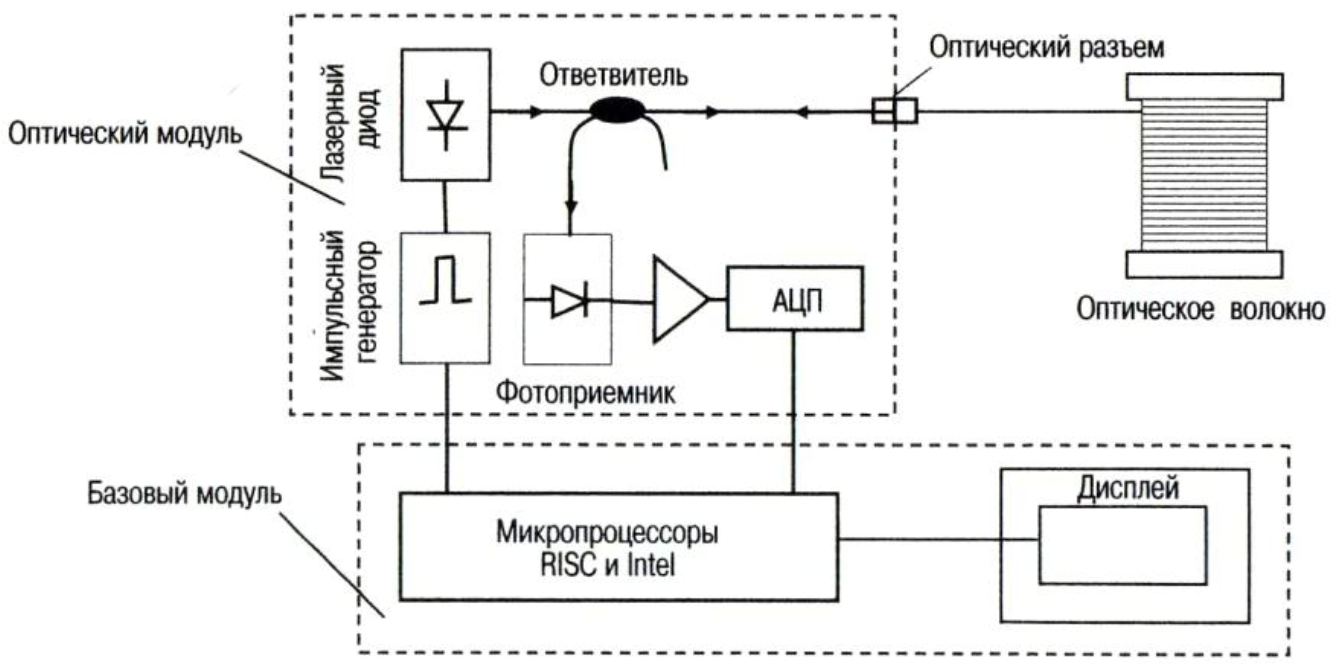
\includegraphics[width=\linewidth]{otdr_schematic}}
  \caption{Блок схема \acrshort{ор}}
  \label{ris:otdr_schematic}
\end{figure}

В качестве источника излучения в оптическом модуле обычно используется лазерные диоды типа Фабри-Перо, наибольшая же мощность излучения (и, соответственно, динамический диапазон рефлектометра) достигается с помощью лазерных диодов с квантовыми ямами. С их помощью генерируются импульсы мощностью 10\dots1000 мВт, длительностью от 2 нс\dots20 мкc и частотой повторения несколько килогерц. Эти импульсы поступают через ответвитель на оптический разъем, к которому подключается исследуемое волокно. Рассеянные в волокне импульсы света возвращаются в оптический модуль и передаются с помощью ответвителя на фотоприемник (лавинный фотодиод), где они преобразуются в электрический сигнал. Этот сигнал усиливается, накапливается, обрабатывается в базовом модуле и отображается на дисплее в графической форме в виде рефлектограммы. Такое представление информации позволяет анализировать её как визуально, так и автоматически с помощью встроенных программных алгоритмов~\cite{listvin:reflectometria}.

\subsection{События на линии}

\acrshort{ор} позволяет находить и отображать на рефлектограмме сварные и механические соединения, коннекторные соединения, изгибы и другие неоднородности волокна. Такие неоднородности называют событиями. 
События могут быть \textbf{отражающими} и \textbf{неотражающими}. 

Потери в разъемных соединениях являются следствием несовершенства как самой конструкции соединителя, так и процесса оконцовывания \acrshort{ов}. Потери в разъемных соединениях зависят от неточности юстировки волокон при их заделке в наконечник соединителя (радиальное, угловое и осевое смещение) и некачественной обработки (полировки) торцов соединяемых \acrshort{ов}. В разъемных соединениях эти потери обычно являются основными.

Потери в неразъемных соединениях определяются неточностью
юстировки \acrshort{ов} в сварочном аппарате перед сваркой. Однако современные сварочные аппараты имеют автоматическую юстировку и автоматическое управление процессом сварки \acrshort{ов}, обеспечивающее минимальные потери. Вследствие этого потери в сварке в основном определяются различием параметров свариваемых \acrshort{ов}~\cite{bilina:izmerenie_parametrov}.

Коннекторные соединения, трещина в волокне или обрыв, образующие поверхность разлома под углом порядка 90º к оси волокна --- примеры отражающих неоднородностей. В этих случаях происходит отражение части исходного излучения в направлении \acrshort{фпу}. На рефлектограмме такие события отображаются в виде пиков. 
Отражающие неоднородности сопровождаются возвратными потерями, которые могут быть рассчитаны по выражению (\ref{eqn:refl_loss}).

\begin{equation}
  \label{eqn:refl_loss}
  \alpha=-10\cdot \lg R
\end{equation}

\noindent где \\
$R$~--- коэффициент отражения.

В отличие от отражающих неоднородностей, в неразъемных соединениях (сварные, клеевые и механические сростки волокон), как правило нет воздушного зазора и отсутствуют отражения. Они отображаются на рефлектограмме ступенькой.

\subsection{Обзор формата SOR (Telecordia SR-4731)}

Наиболее распространенным форматом для хранения результатов измерения оптических рефлектометров является формат SOR (Standard OTDR Record) Telecordia SR-4731.
Он читается всеми приложениями для обработки рефлектограмм. Альтернативным форматом является TRC, с ним в частности работают приборы компании EXFO~\cite{web:volsexpert_reflectometria}.

Данный стандарт предусматривает следующие блоки~\cite{web:otdr_format}:

\subsubsection{Блок общих параметров}

Блок состоит из следующих полей:
\begin{itemize}
  \item id кабеля;
  \item id \acrshort{ов};
  \item тип \acrshort{ов};
  \item длина волны;
  \item точка А;
  \item точка Б;
  \item код кабеля;
  \item состояние кабеля, одно из значений:
  \begin{itemize}
    \item \textbf{BC}: как проложен;
    \item \textbf{CC}: текущее;
    \item \textbf{RC}: после ремонта;
    \item \textbf{OT}: иное.
  \end{itemize}
  \item пользовательский отступ;
  \item расстояние до пользовательского отступа;
  \item оператор;
  \item комментарии.
\end{itemize}

\subsubsection{Блок поставщика оптического рефлектометра}

Блок состоит из следующих полей:
\begin{itemize}
  \item наименование поставщика;
  \item наименование \acrshort{ор};
  \item серийный номер \acrshort{ор};
  \item название модуля;
  \item серийный номер модуля;
  \item версия \acrshort{по};
  \item прочее.
\end{itemize}

\subsubsection{Блок фиксированных параметров}
\label{fixed_params_block}

Блок состоит из следующих полей:
\begin{itemize}
  \item дата и время создания рефлектограммы (количество секунд прошедших с 1 января 1970 г.);
  \item единицы измерения, одно из значений:
  \begin{itemize}
    \item \textbf{km}: километры;
    \item \textbf{mt}: метры;
    \item \textbf{ft}: футы;
    \item \textbf{kf}: килофуты;
    \item \textbf{mi}: мили.
  \end{itemize}
  \item количество длин пульсов (на случай, если в файле несколько рефлектограмм);
  \item длина пульса (повторяется столько раз, сколько указано в пункте выше) (нс);
  \item разброс между измерений (делить на $10$, чтобы получить фс);
  \item количество измерений;
  \item показатель преломления;
  \item коэффициент обратного рассеяния (умножить на $-0,1$, чтобы получить дБ);
  \item время усреднения (с);
  \item дальность (умножить на $2\cdot 10^{-5}$, чтобы получить км);
  \item уровень шума;
  \item порог потерь (умножить на $0,001$, чтобы получить дБ);
  \item порог отражения (умножить на $-0,001$, чтобы получить дБ);
  \item порог конца передачи (умножить на $0,001$, чтобы получить дБ);
  \item тип рефлектограммы, одно из значений:
  \begin{itemize}
    \item \textbf{ST}: стандартная рефлектограмма;
    \item \textbf{RT}: обратная рефлектограмма;
    \item \textbf{DT}: разница рефлектограмм;
    \item \textbf{RF}: образец.
  \end{itemize}
\end{itemize}

\subsubsection{Блок ключевых событий}

Cледующие поля повторяются для каждого события:
\begin{itemize}
  \item номер события;
  \item время до события (умножить на $0,1$, чтобы получить нс);
  \item затухание (умножить на $0,001$, чтобы получить дБ/км);
  \item потери сварки (умножить на $0,001$, чтобы получить дБ);
  \item потери отражения (умножить на $0,001$, чтобы получить дБ);
  \item тип события, одно из полей:
  \begin{itemize}
    \item \textbf{0}: ступенька вверх или вниз;
    \item \textbf{1}: отражение;
    \item \textbf{2}: множественное событие.
  \end{itemize}
  \item конец предыдущего события (0, если первое событие);
  \item начало события;
  \item конец события;
  \item начало следующего события (равно дальности, если последнее событие);
  \item пик текущего события;
  \item комментарий.
\end{itemize}

После ключевых событий следующий блок значений:
\begin{itemize}
  \item суммарное затухание (умножить на $0,001$, чтобы получить дБ);
  \item начало \acrshort{ов};
  \item протяженность \acrshort{ов};
  \item потери отражения (умножить на $0,001$, чтобы получить дБ).
\end{itemize}

Зная время до события можно рассчитать расстояние до него по формуле~(\ref{eqn:event_distance})

\begin{equation}
  \label{eqn:event_distance}
  d = t \cdot \frac{c}{n}
\end{equation}

\noindent где \\
$t$~--- время до события \\
$c$~--- скорость света \\
$n$~--- показатель преломления

\subsubsection{Блок точек}

В начале блока идет количество точек (совпадает с количеством измерений указанным в пункте \ref{fixed_params_block}), после этого идет количество рефлектограмм (совпадает с количеством длин пульсов указанным в пункте \ref{fixed_params_block}). Далее идут измерения~--- дБ и соответственные расстояния.

\subsubsection{Блок контрольной суммы}

Контрольная сумма вычисленная по алгоритму CRC-16.

\subsection{Анализ существующих решений}

Распространенные в данный момент аналоги не является кросс платформенными, что значит они не имееют возможность выполняться во всех популярных операционных системах (Window, OSX, Linux) и на всех поддерживаемых этими платформами архитектурах.

\subsubsection{EXFO FastReporter и EXFO LiteReporter}

\textbf{Ключевой функционал:} \cite{web:fastreporter_specs}
\begin{itemize}
  \item автопоиск событий;
  \item создание эталонных рефлектограмм;
  \item обработка наборов рефлектограмм;
  \item двунапраленный анализ;
  \item интеграция с облачными сервисами.
\end{itemize}

Поддерживаемые операционные системы: \textbf{Windows}.

\begin{figure}[H]
  \center{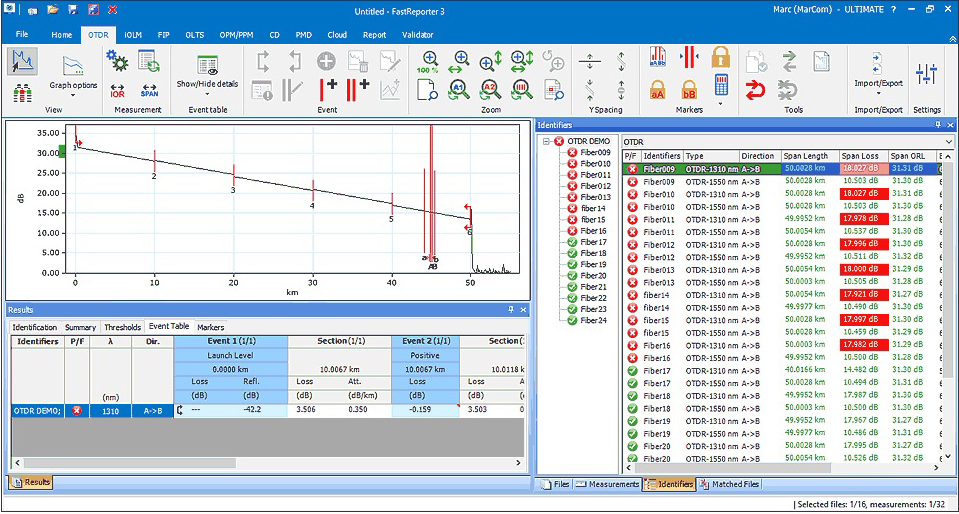
\includegraphics[width=\linewidth]{fastreporter}}
  \caption{Интерфейс программы FastReporter}
  \label{ris:fastreporter}
\end{figure}

\subsubsection{VIAVI Solutions Fiber Trace Viewer}

\textbf{Ключевой функционал:} \cite{web:viavi}
\begin{itemize}
  \item автопоиск событий;
  \item обработка наборов рефлектограмм;
  \item двунапраленный анализ.
\end{itemize}

Поддерживаемые операционные системы: \textbf{Windows}.

\subsubsection{Yokogawa Electric Corporation AQ 7933}

\textbf{Ключевой функционал:} \cite{web:yokogawa}
\begin{itemize}
  \item автопоиск событий;
  \item обработка наборов рефлектограмм;
  \item двунапраленный анализ;
  \item создание событий.
\end{itemize}

Поддерживаемые операционные системы: \textbf{Windows}.

\begin{figure}[H]
  \center{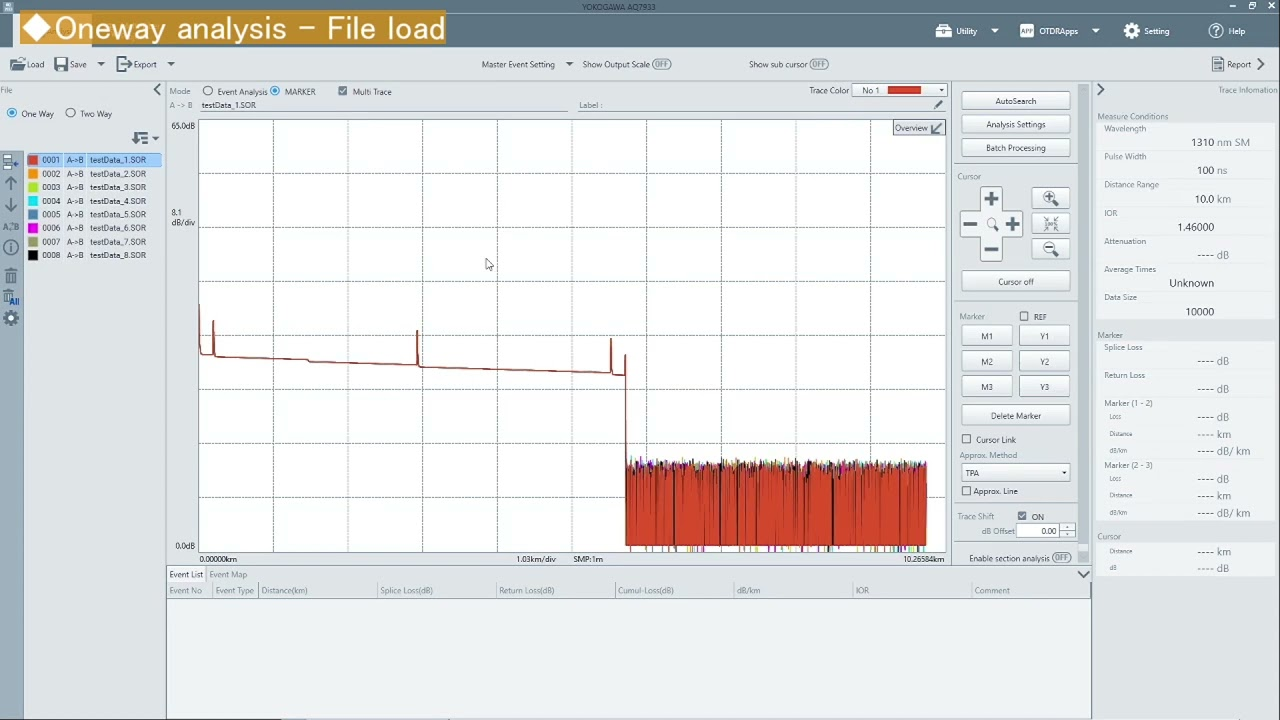
\includegraphics[width=\linewidth]{Yokogawa_Electric_Corporation_AQ_7933}}
  \caption{Интерфейс программы Yokogawa Electric Corporation AQ 7933}
  \label{ris:yokogawa}
\end{figure}

\subsubsection{СвязьСервис TopOTDRViewer}

\textbf{Ключевой функционал:} \cite{web:topotdrviewer}
\begin{itemize}
  \item автопоиск событий;
  \item обработка наборов рефлектограмм.
\end{itemize}

Поддерживаемые операционные системы: \textbf{Windows}.

\begin{figure}[H]
  \center{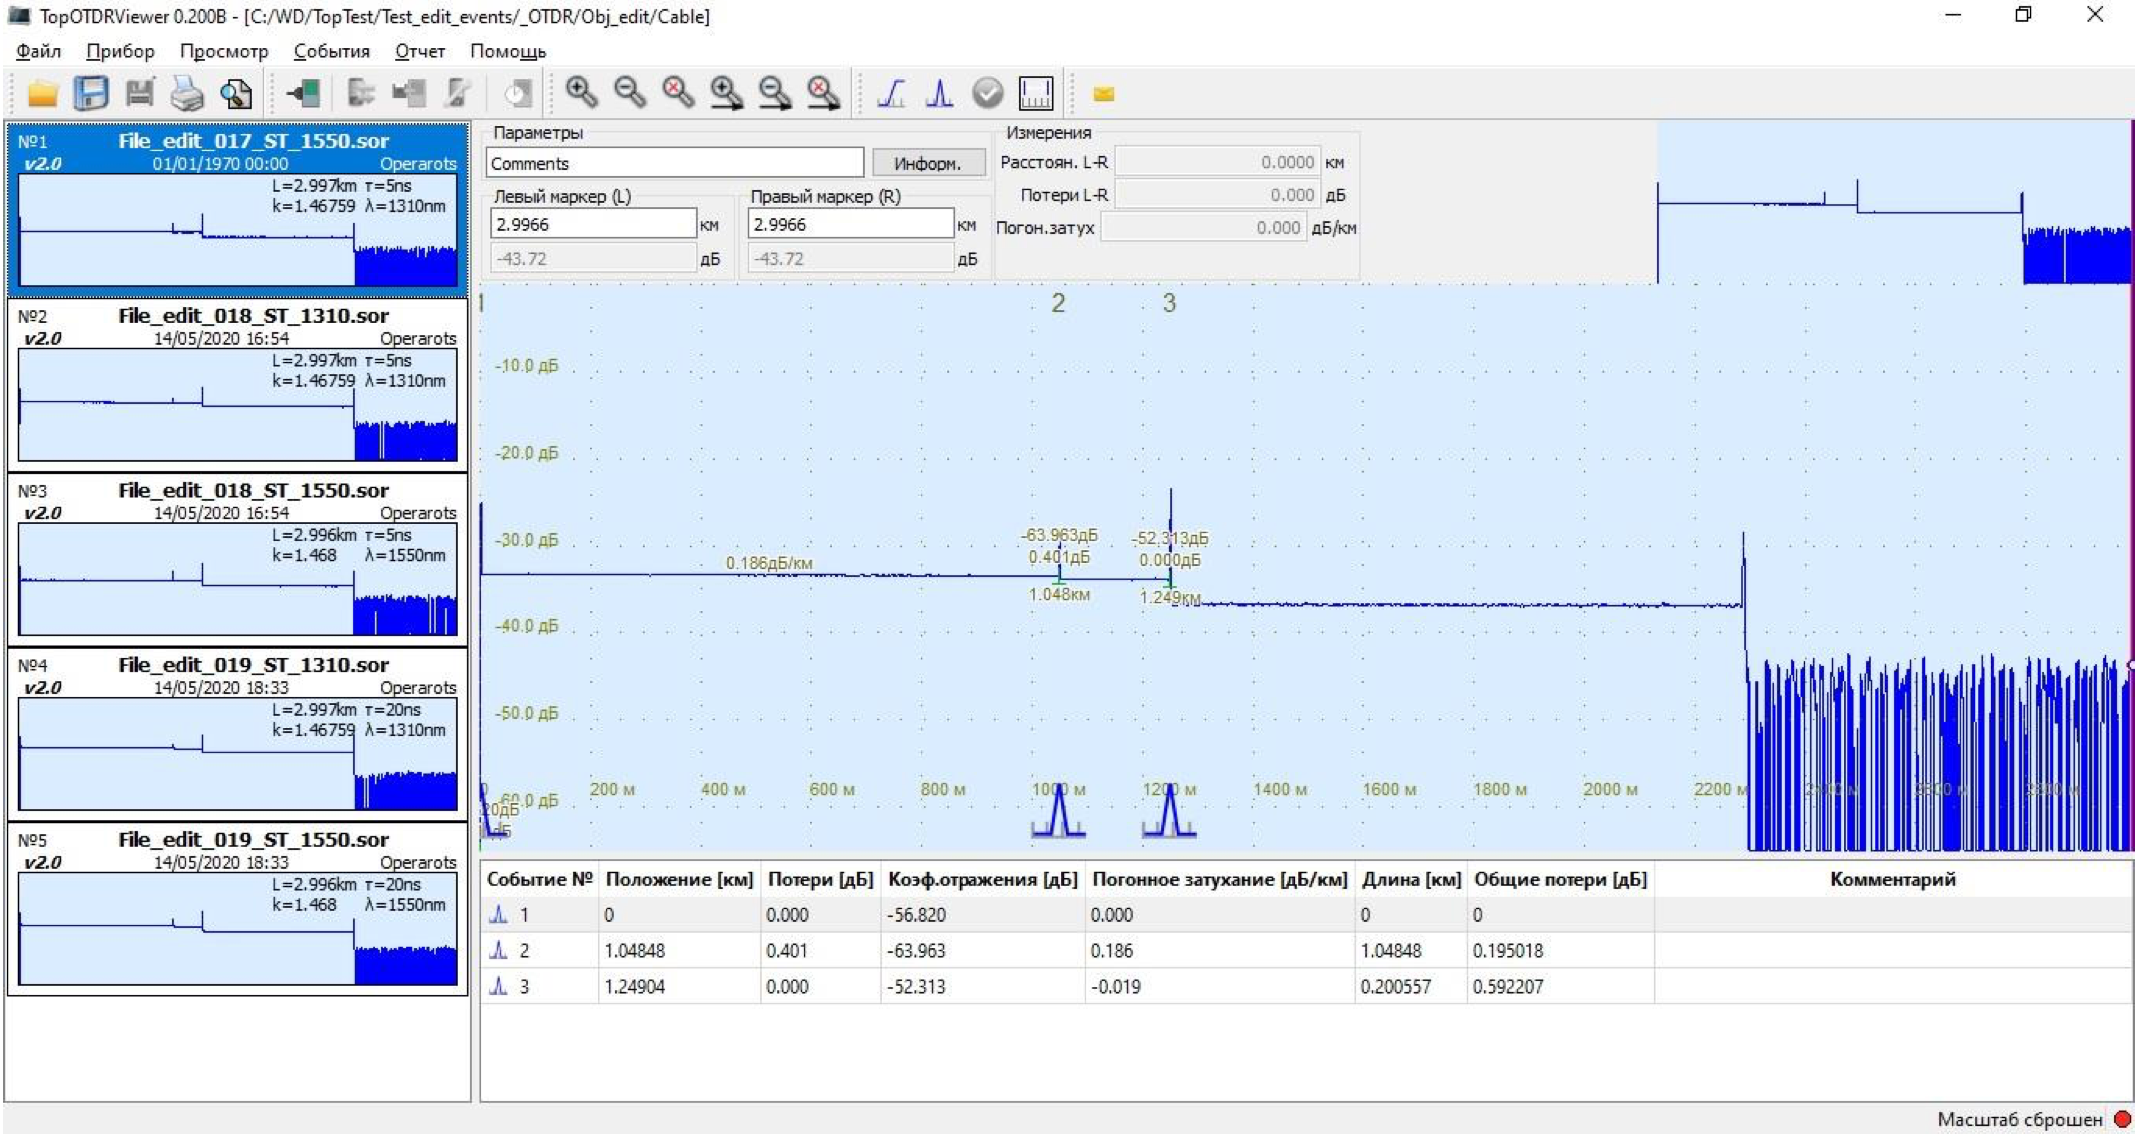
\includegraphics[width=\linewidth]{topotdrviewer}}
  \caption{Интерфейс программы TopOTDRViewer}
  \label{ris:topotdrviewer}
\end{figure}

\subsubsection{SORTraceViewer}

\textbf{Ключевой функционал:} \cite{web:sortraceviewer}
\begin{itemize}
  \item автопоиск событий;
  \item двунапраленный анализ;
  \item обработка наборов рефлектограмм;
  \item редактирование точек рефлектограммы.
\end{itemize}

Поддерживаемые операционные системы: \textbf{Windows}, \textbf{Linux}.

\begin{figure}[H]
  \center{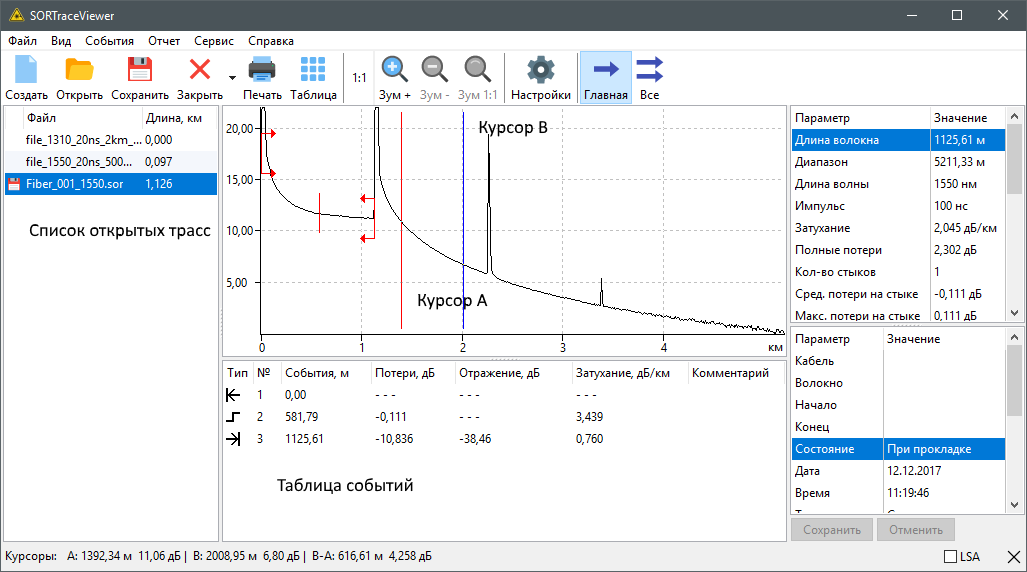
\includegraphics[width=\linewidth]{sortraceviewer}}
  \caption{Интерфейс программы SORTraceViewer}
  \label{ris:sortraceviewer}
\end{figure}

\subsection{Выводы по разделу}

В разделе описана предметная область, рассмотрено устройство рефлектометра, а также формат данных в которых сохраняются результаты измерения. Помимо этого рассмотрены существующие программы для обработки результатов измерений \acrshort{ор}.


\newpage
\section{РАЗРАБОТКА ПРОГРАММНОГО ОБЕСПЕЧЕНИЯ}
\subsection{Требования к разрабатываемому программному обеспечению}

Приложение имеет возможность открывать файлы результатов измерений \acrshort{ор}.
При открытии приложения пользователю доступна кнопка <<Открыть файл>>, по нажатию которой открывается файловый менеджер, в котором можно выбрать файл для открытия.
После открытия файла открывается главный \gls{вид} приложения, на нем отображаются следующие элементы управления:
\begin{itemize}
  \item график рефлектограммы;
  \item кнопка <<Библиотека файлов>>;
  \item кнопка <<Открыть файл>>;
  \item кнопка <<Сгенерировать рефлектограмму>>;
  \item кнопка <<Сохранить в библиотеку>>;
  \item поле ввода <<Лимит отражения>>;
  \item поле ввода <<Лимит поглощения>>;
  \item поле ввода <<Лимит Тигера>>;
  \item переключение отображения встроенных событий;
  \item переключение отображения найденных событий методом 1;
  \item переключение отображения найденных событий методом \acrshort{teo};
  \item переключение отображения графика результата преобразования \acrshort{teo}.
\end{itemize}

Назначение перечисленных элементов:

\subsubsection{График рефлектограммы}

Отображает рефлектограмму из открытого файла. Нажатие на рефлектограмму открывает \gls{модальное окно} содержащее следующие компоненты:

\begin{itemize}
  \item селектор <<Отражающее / неотражающее событие>>;
  \item поле ввода <<Потери>>;
  \item поле ввода <<Отражение>>;
  \item кнопка <<Закрыть>>;
  \item кнопка <<Обрезать рефлектограмму>>;
  \item кнопка <<Добавить событие>>.
\end{itemize}

Назначение перечисленных элементов (до пункта \ref{добавить_событие}):

\subsubsection{Селектор  <<Отражающее / неотражающее событие>>}

Переключение выбирает то, какое событие будет добавлено на рефлектограммму при нажатии на кнопку <<Добавить событие>>.

\subsubsection{Поле ввода <<Потери>>}

Задает количество дБ, на которое уменьшится мощность сигнала после события.

\subsubsection{Поле ввода <<Отражение>>}

Задает количество дБ, которому будет соответствовать величина обратных отражений, если будет добавлено отражающее событие.

\subsubsection{Кнопка <<Закрыть>>}

Закрывает \gls{модальное окно}.

\subsubsection{Кнопка <<Обрезать рефлектограмму>>}
\label{обрезать_рефлектограмму}

Закрывает \gls{модальное окно} и обрезает рефлектограмму в выбранном пользователем месте.

\subsubsection{Кнопка <<Добавить событие>>}
\label{добавить_событие}

Закрывает \gls{модальное окно} и добавляет пользовательское событие в выбранном месте, с параметрами соответствующим селектору <<Отражающее / неотражающее событие>> и полям <<Потери>> и <<Отражение>>.

\subsubsection{Кнопка <<Библиотека файлов>>}

Открывает \gls{вид} <<Библиотека файлов>>. На экране располагается список сохраненных ранее файлов. У каждого файла указаны его название, дата снятия измерений, id кабеля, id волокна, длина волны, коментарии к файлу.

Клик по элементу списка открывает главный \gls{вид} с соотретствующей рефлектограммой.

\subsubsection{Кнопка <<Открыть файл>>}

Дублирует функционал кнопки доступной при первоначальном запуске приложения.

\subsubsection{Кнопка <<Сохранить в библиотеку>>}

Имеет 2 состояния:
\begin{itemize}
  \item Если файл не сохранен в библиотеке приложения, то:
  
  отображается текст <<Сохранить в библиотеку>>. По нажатию открытый в данный момент файл сохраняется в библиотеку приложения и становится доступным на \glslink{вид}{виде} <<Библиотека файлов>>;
  \item если файл уже сохранен в библиотеке приложения, то:
  
  отображается текст <<Файл в библиотеке>>.
\end{itemize}

\subsubsection{Кнопка <<Сгенерировать рефлектограмму>>}

Открывает \gls{модальное окно}, в котором содержатся следующие компоненты:

\begin{itemize}
  \item поле ввода <<Затухание>>;
  \item поле ввода <<Масштаб шума>>;
  \item кнопка <<Закрыть>>;
  \item кнопка <<Сгенерировать>>.
\end{itemize}

Назначение перечисленных элементов (до пункта \ref{сгенерировать}):

\subsubsection{Поле ввода <<Затухание>>}

Задает километрическое затухание, которое будет использовано для генерации рефлектограммы.

\subsubsection{Поле ввода <<Масштаб шума>>}

Задает степень зашумленности создаваемого сигнала.

\subsubsection{Кнопка <<Закрыть>>}

Закрывает \gls{модальное окно}.

\subsubsection{Кнопка <<Сгенерировать>>}
\label{сгенерировать}

Закрывает \gls{модальное окно} и продолжает рефлектограмму с места, где она была обрезана инструментом <<Обрезать рефлектограмму>> (пункт \ref{обрезать_рефлектограмму})

\subsubsection{Поле ввода <<Лимит отражения>>}

Задает количество дБ, на которое измерение должно отличаться от предыдущего, чтобы классифицироваться как отражающее событие.

\subsubsection{Поле ввода <<Лимит поглощения>>}

Задает количество дБ, на которое измерение должно отличаться от предыдущего, чтобы классифицироваться как неотражающее событие.

\subsubsection{Поле ввода <<Лимит Тигера>>}

Задает количество дБ, которое должно превысить преобразованное оператором Тигера измерение, чтобы классифицироваться как событие.

\subsubsection{Переключатели отображения событий}

Представлены три пункта соответствующие доступным к отображению видам событий:
\begin{itemize}
  \item встроенные события~--- события которые были обнаружены и записаны в файл встроенным в \acrshort{ор} компьютером;
  \item простые события~--- события найденные методом описанным в главе \ref{простой_алгоритм};
  \item простые события~--- события найденные методом описанным в главе \ref{тео_алгоритм}.
\end{itemize}

\subsection{Описание необходимых библиотек и разработанных модулей}

Выбранные библиотеки для разработки приложения на стеке Electron + Vue + Typescript:

\begin{itemize}
  \item Electron версии 21.3.3~--- \gls{фреймворк} для разработки приложений с помощью web технологий;
  \item Vue версии 3.2.45~--- \gls{фреймворк} для разработки \glslink{реактивность}{реактивных} веб приложений;
  \item Typescript версии 4.9.4~--- язык программирования со строгой типизацией данных, который \glslink{транспиляция}{транспилируется} в Javascript;
  \item jsOTDR~--- библиотека для чтения содержимого файлов .sor с преобразованием в json;
  \item d3 версии 7.8.2~--- библиотека для визуализации данных.
  \item Pinia версии 2.1.3~--- библиотека для управления состоянием приложения для Vue;
  \item Vuetify версии 3.1.2~--- \gls{фреймворк} компонентов для Vue.
  \item Vite версии 4.0.4~--- инструмент сборки.
\end{itemize}

\subsection{Алгоритм поиска событий}

В программе реализовано 2 алгоритма поиска событий. Пользователю доступна возможность включить любой из них или оба, либо выключить оба.

\subsubsection{Простой алгоритм} \label{простой_алгоритм}

Алгоритм поиска событий основан на том, чтобы вычислить для каждого дискретного измерения рефлектометра соответствующее ему затухание относительно предыдущего измерения. Отражающие события можно достаточно просто определить если мощность в точке $n$ превышает мощность в точке $n-1$ на одну величину. А неотражающие события соответственно можно определить как падение мощности, превышающее другую величину (\ref{eqn:naive}). В большинстве рефлектометров встроенный компьютер использует в качестве этого значения $0,01 \text{ дБ}$.

\begin{equation}
  \label{eqn:naive}
  \left\{
    \begin{array}{ll}
      S_n - S_{n+1} > k_1 & \text{при } S_{n+1} \leqslant S_n \\
      S_n - S_{n+1} > k_2 & \text{при } S_{n+1} > S_n
    \end{array}
  \right.
\end{equation}

\subsubsection{Aлгоритм на основе энергетического оператора Тигера} \label{тео_алгоритм}

Альтернативным подходом к поиску событий может служить использование энергетического оператора Тигера (\acrshort{teo})~\cite{lima:teo}. Его значение для дискретного сигнала равно разнице квадрата значения в точке $n$ и произведению значений в точках $n-1$ и $n+1$ (\ref{eqn:teo}). Такой оператор очень чувствителен к изменениям и с правильно выставленным пороговым значением позволяет находить события с высокой точностью.

\begin{equation}
  \label{eqn:teo}
  \Psi[S_n] = S_n^2-S_{n-1}\cdot S_{n+1}
\end{equation}

\subsection{Реализация редактирования рефлектограммы}

\subsubsection{Обрезка рефлектограммы}

При клике на рефлектограмму вычисляется величина обратная масштабу отображения рефлектограммы и используется для того, чтобы найти элемент в массиве измеренных величин, который был кликнут. Все значения после него удаляются.

\subsubsection{Генерация рефлектограммы}

В формате SOR предусмотрено поле \mintinline{js}|info.DataPts["num data points"]|, которое содержит количество измерений сделанных \acrshort{ор}.
Программа последовательно добавляет к существующей рефлектограмме значения с соответствующими параметрами $x$ и $y$, до тех пор, пока количество значений не достигнет изначальной величины \mintinline{js}|info.DataPts["num data points"]|:

\begin{equation}
  \label{eqn:generate_x}
  x_n = x_{n-1} + r
\end{equation}

\begin{equation}
  \label{eqn:generate_y}
  y_n = y_{n-1} + \alpha \cdot r + t
\end{equation}

\noindent где \\
$\alpha$~--- километрическое затухание (дБ/км) \\
$r$~--- разшешение рефлектометра \\
$t$~--- шум

\subsubsection{Добавление событий}

Программа уменьшает мощность всех измерений следующих после события на заданную пользователем величину. 
Если добавляется отражающее событие, то в точке события мощность нескольких измерений увеличивается на заданную величину.

\subsection{Результат разработки}

В результате разработки в соответствии с требованиями было разработано приложение со следующими характеристиками:

\begin{itemize}
  \item приложение открывает файлы .sor;
  \item приложение отображает рефлектограммы открытых файлов;
  \item на рефлектограммах отображаются события:
  \begin{itemize}
    \item встроенные;
    \item найденные простым подходом;
    \item найденные с помощью \acrshort{teo}.
  \end{itemize}
  \item рефлектограмму можно обрезать в выбранном пользователем месте;
  \item на рефлектограмму можно добавить отражающее или неотражающее событие с заданными параметрами;
  \item в приложение встроена система организации результатов измерения \acrshort{ор};
  \item сохраненные результаты измерений можно просматривать и открывать из встроенной в программу библиотеки;
  \item приложение работает на операционных системах Windows, Mac OS и Linux.
\end{itemize}

\subsection{Выводы по разделу}

В разделе приведено описание необходимых библиотек и разработанных модулей, кратко представлены результаты разработки.


\newpage
\section{ДЕМОНСТРАЦИЯ РАБОТЫ ПРИЛОЖЕНИЯ}

\subsection{Функция <<Открыть файл>>}

\begin{figure}[H]
  \center{\frame{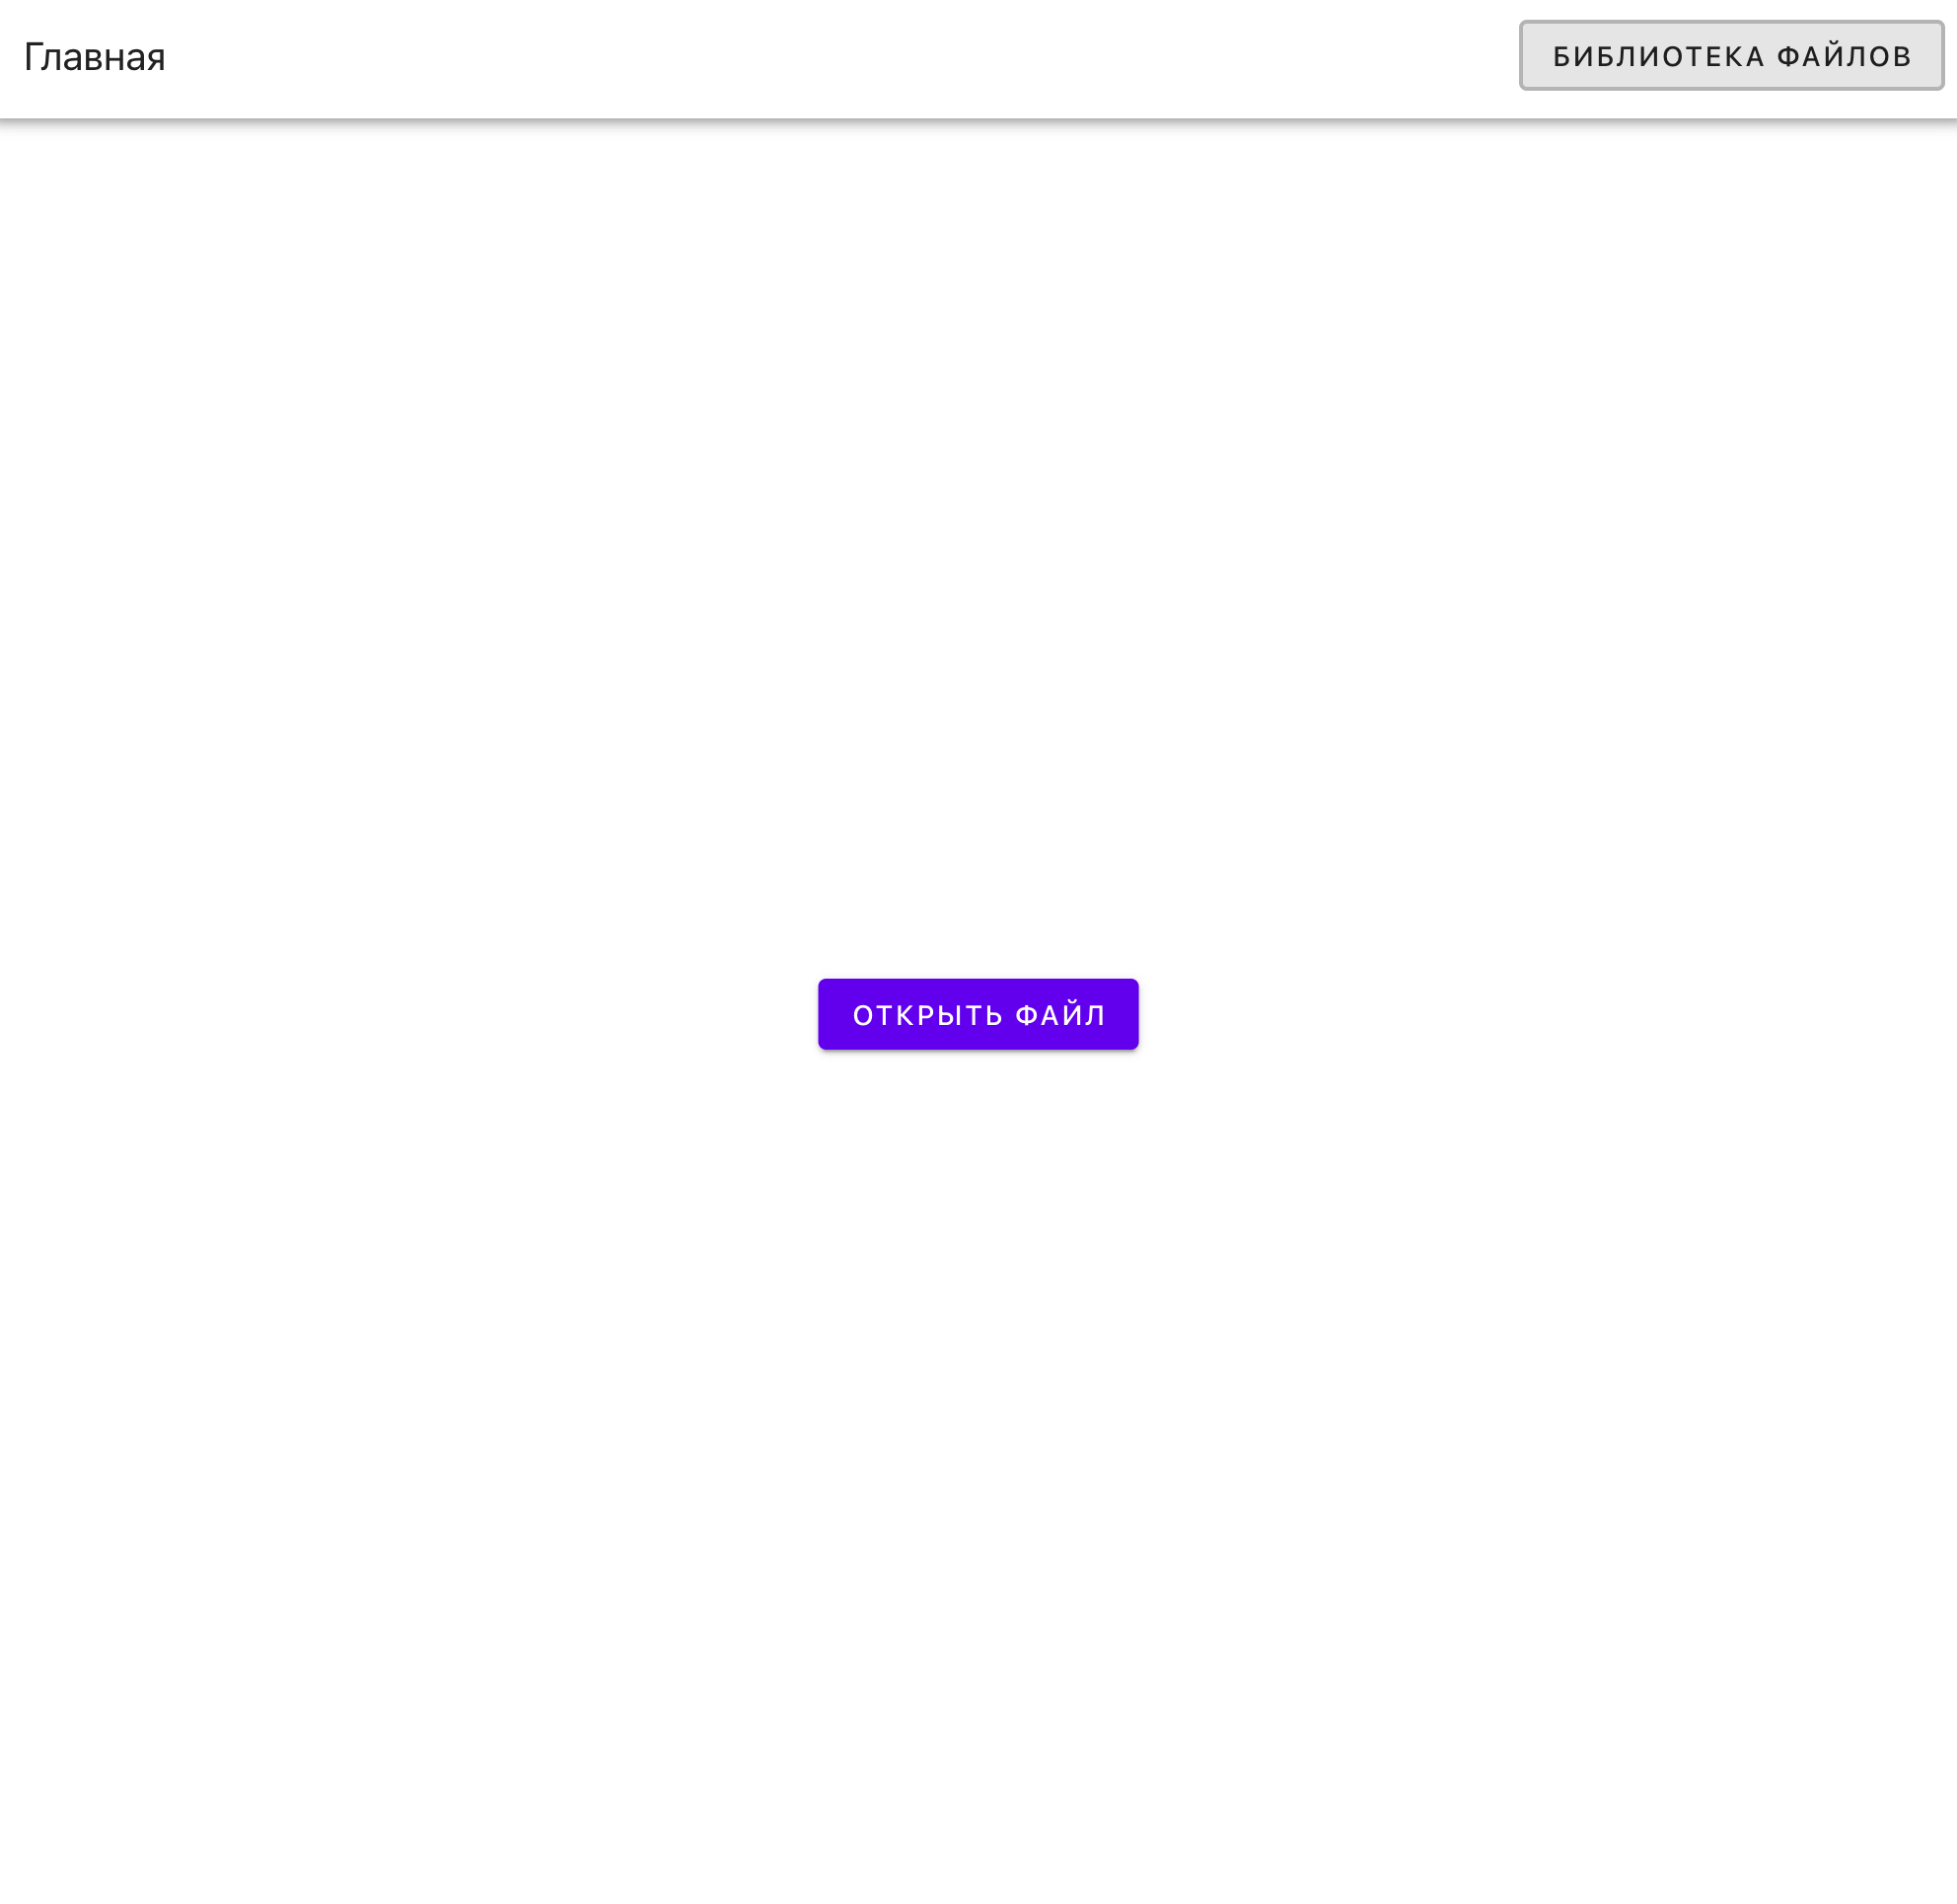
\includegraphics[width=0.65\textwidth]{startup}}}
  \caption{Интерфейс программы при запуске}
  \label{ris:startup}
\end{figure}


\begin{figure}[H]
  \center{\frame{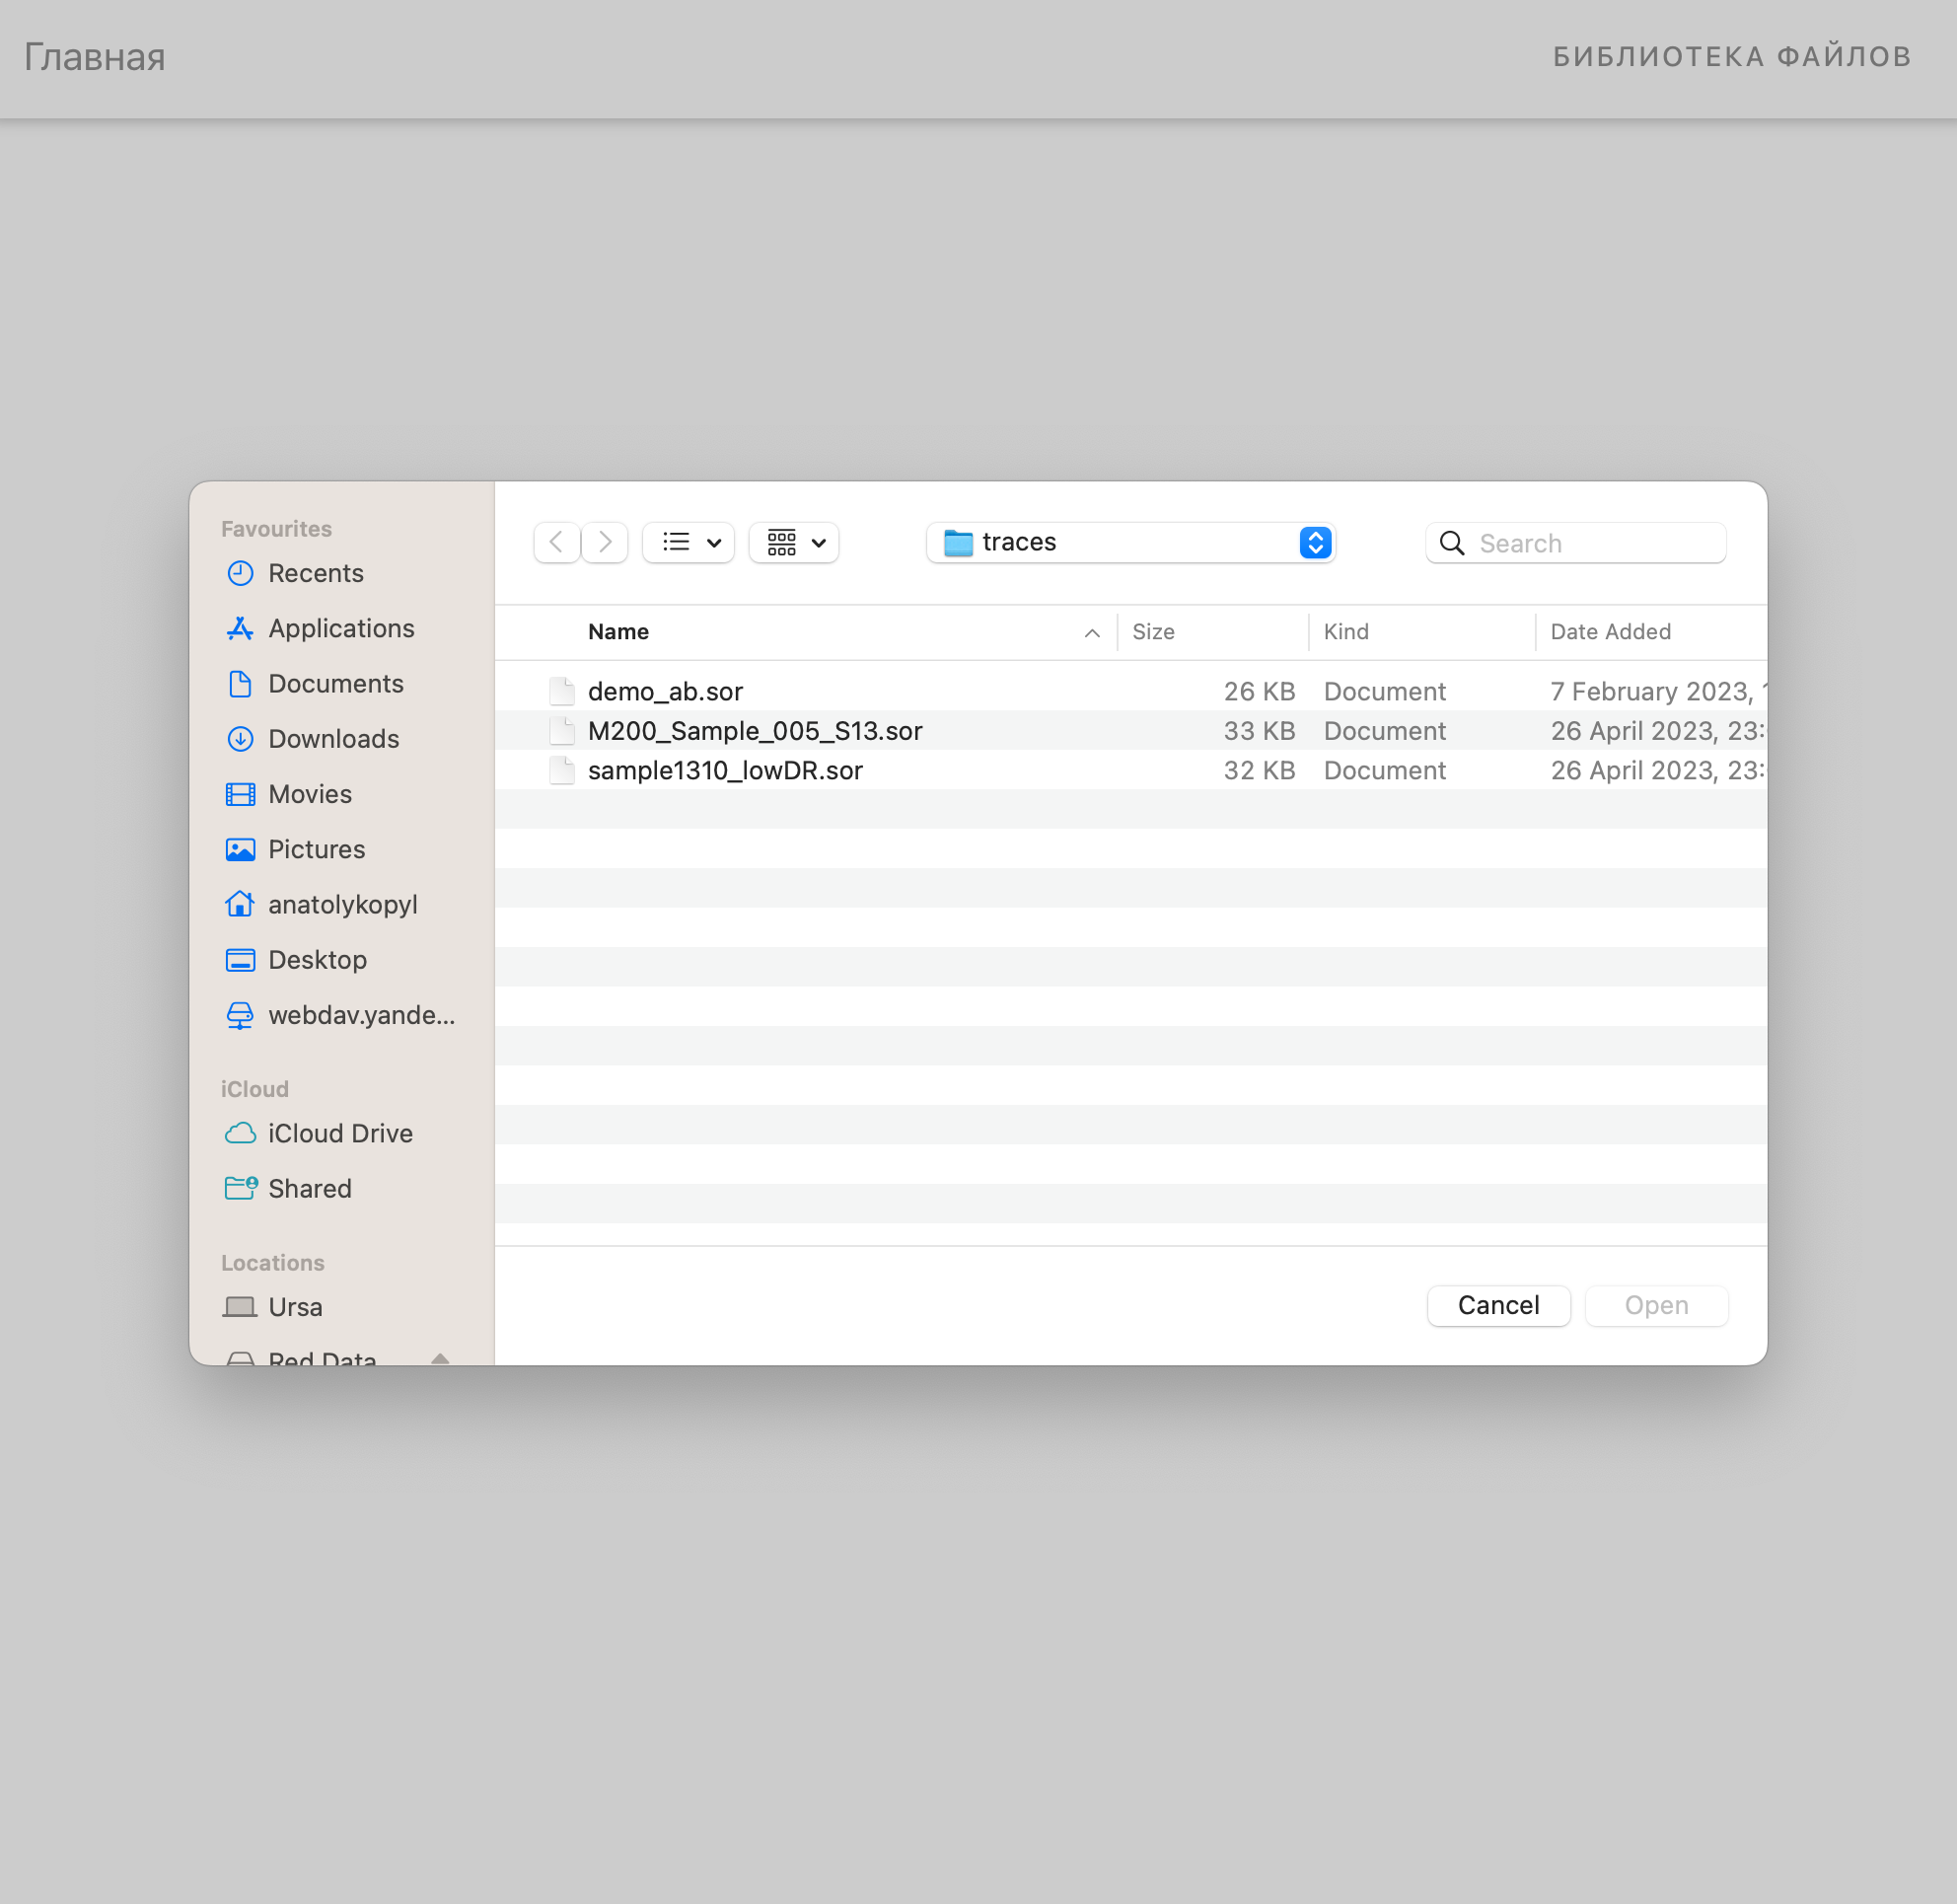
\includegraphics[width=0.65\textwidth]{file_manager}}}
  \caption{Файловый менеджер}
  \label{ris:file_manager}
\end{figure}

\begin{figure}[H]
  \center{\frame{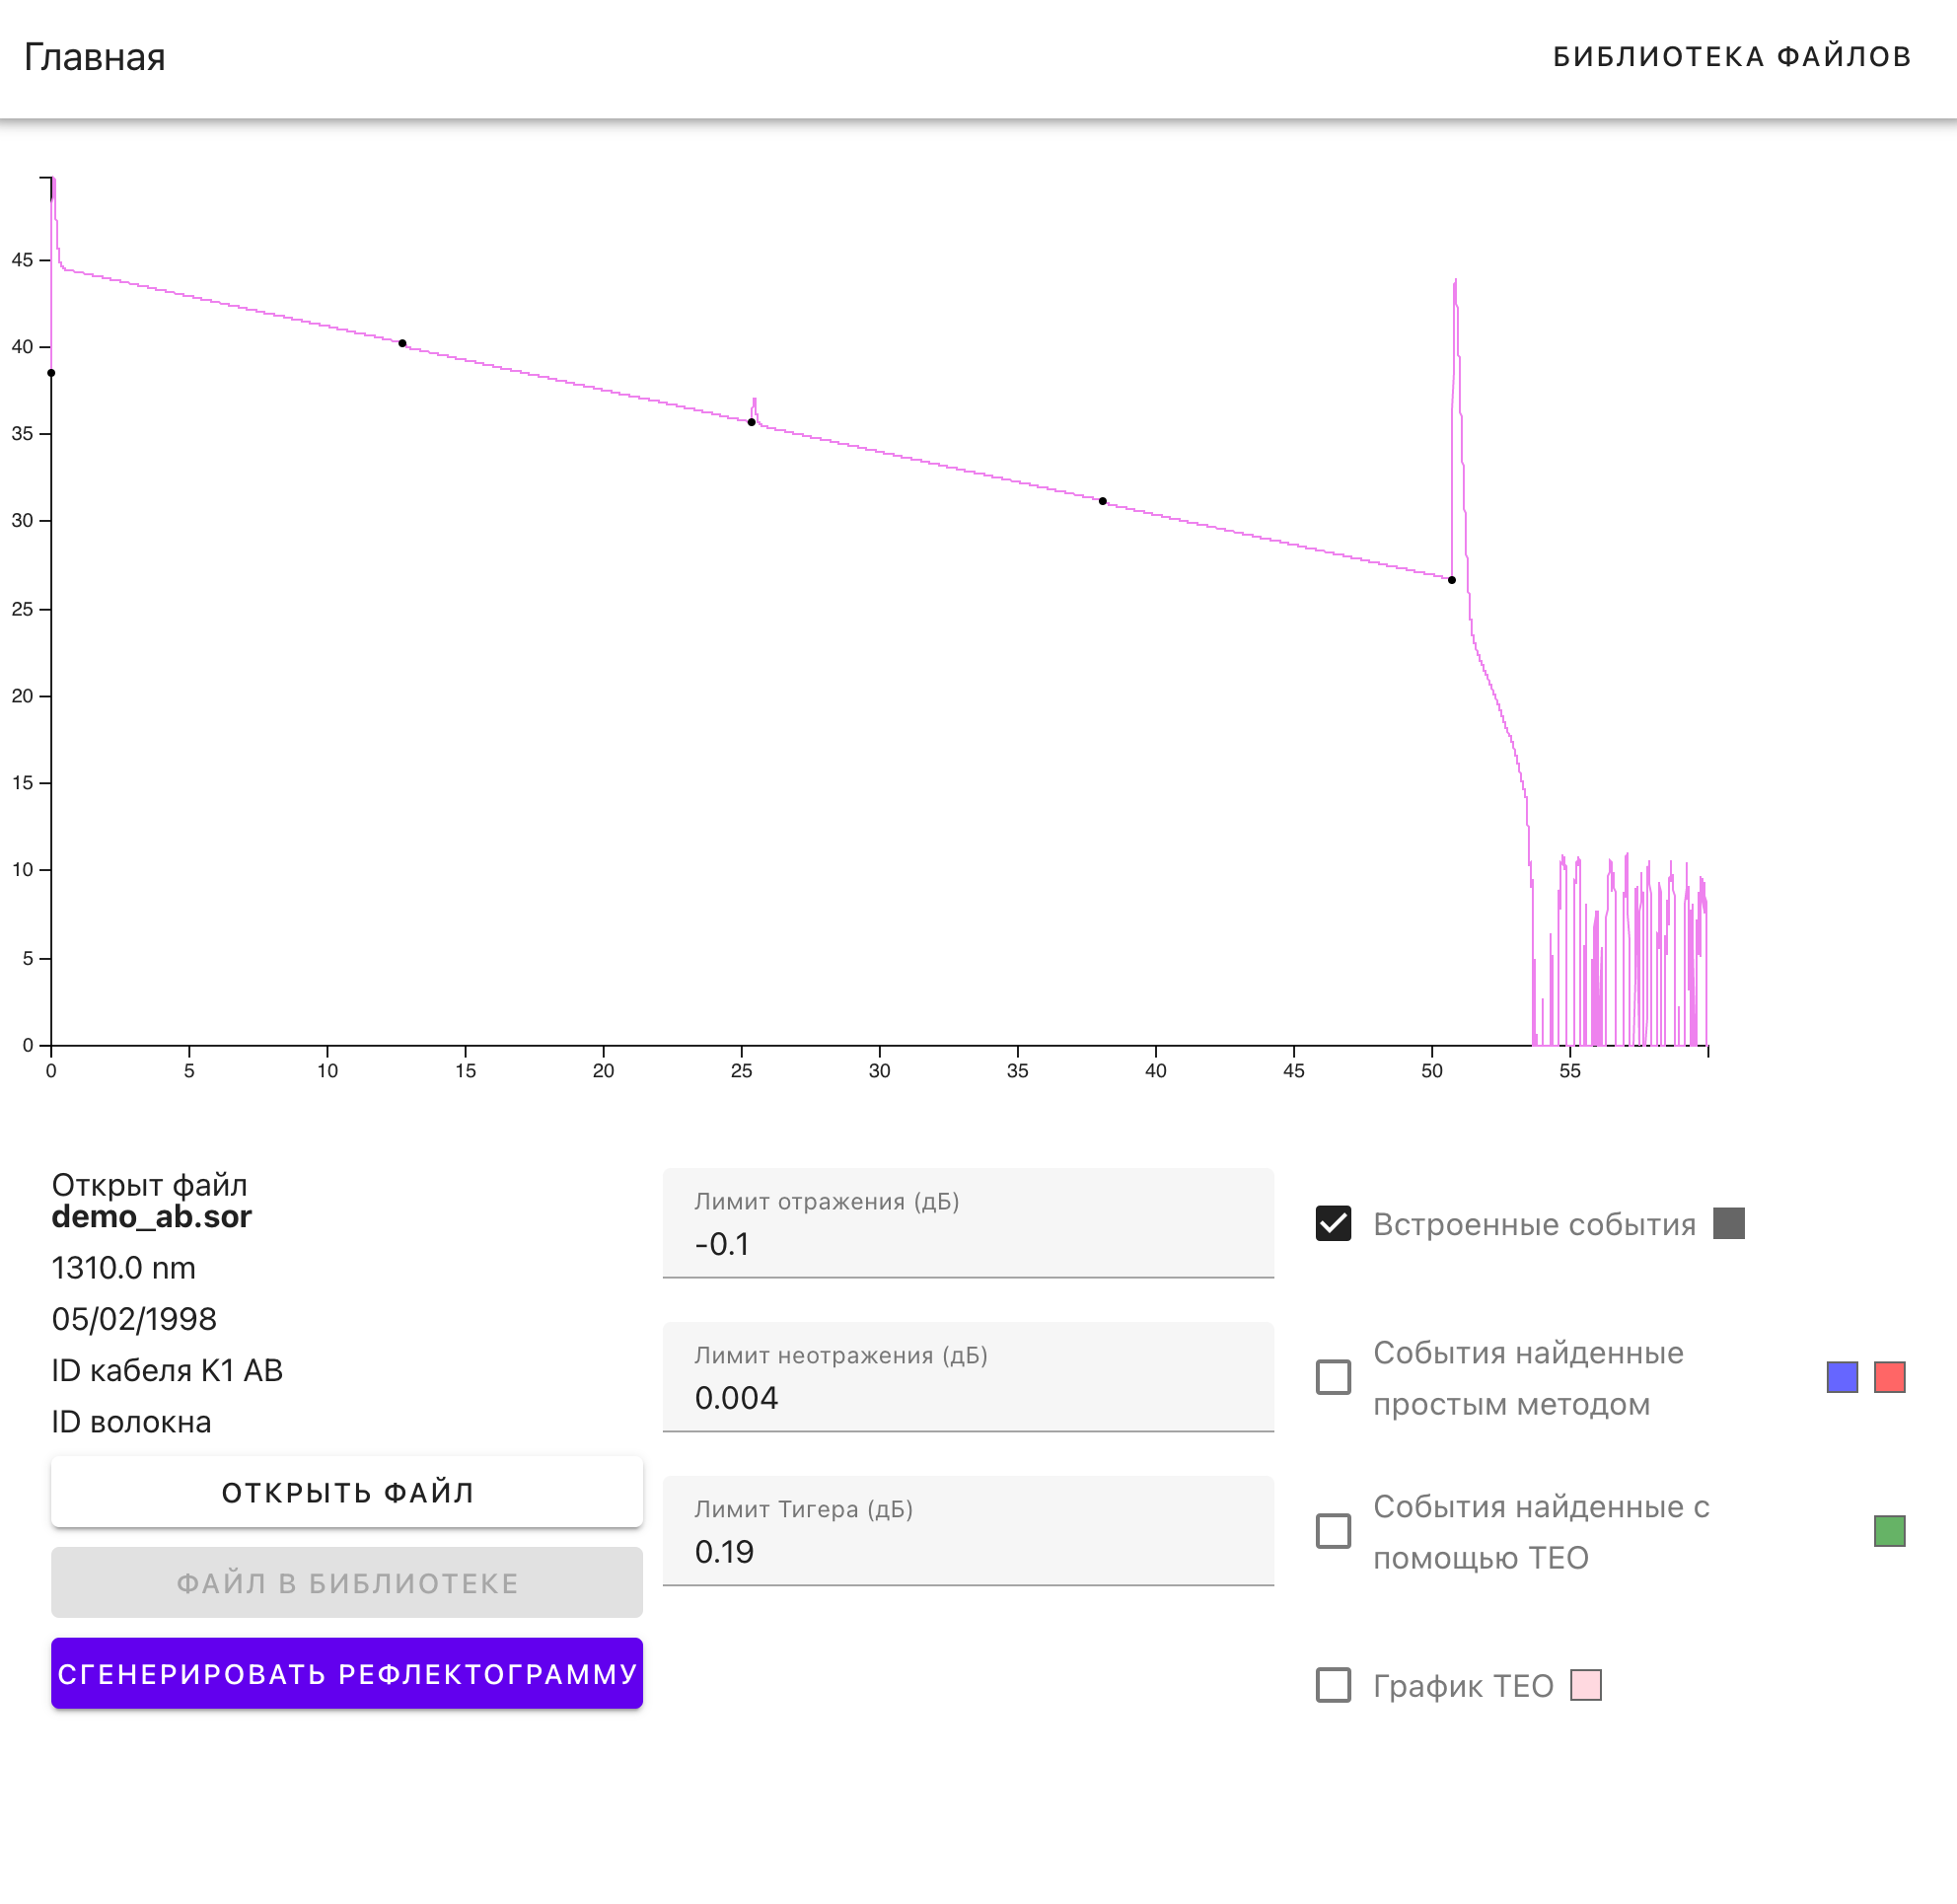
\includegraphics[width=0.65\textwidth]{opened_file}}}
  \caption{Файл открыт}
  \label{ris:opened_file}
\end{figure}

\subsection{Функция <<Поиск событий>>}

\begin{figure}[H]
  \center{\frame{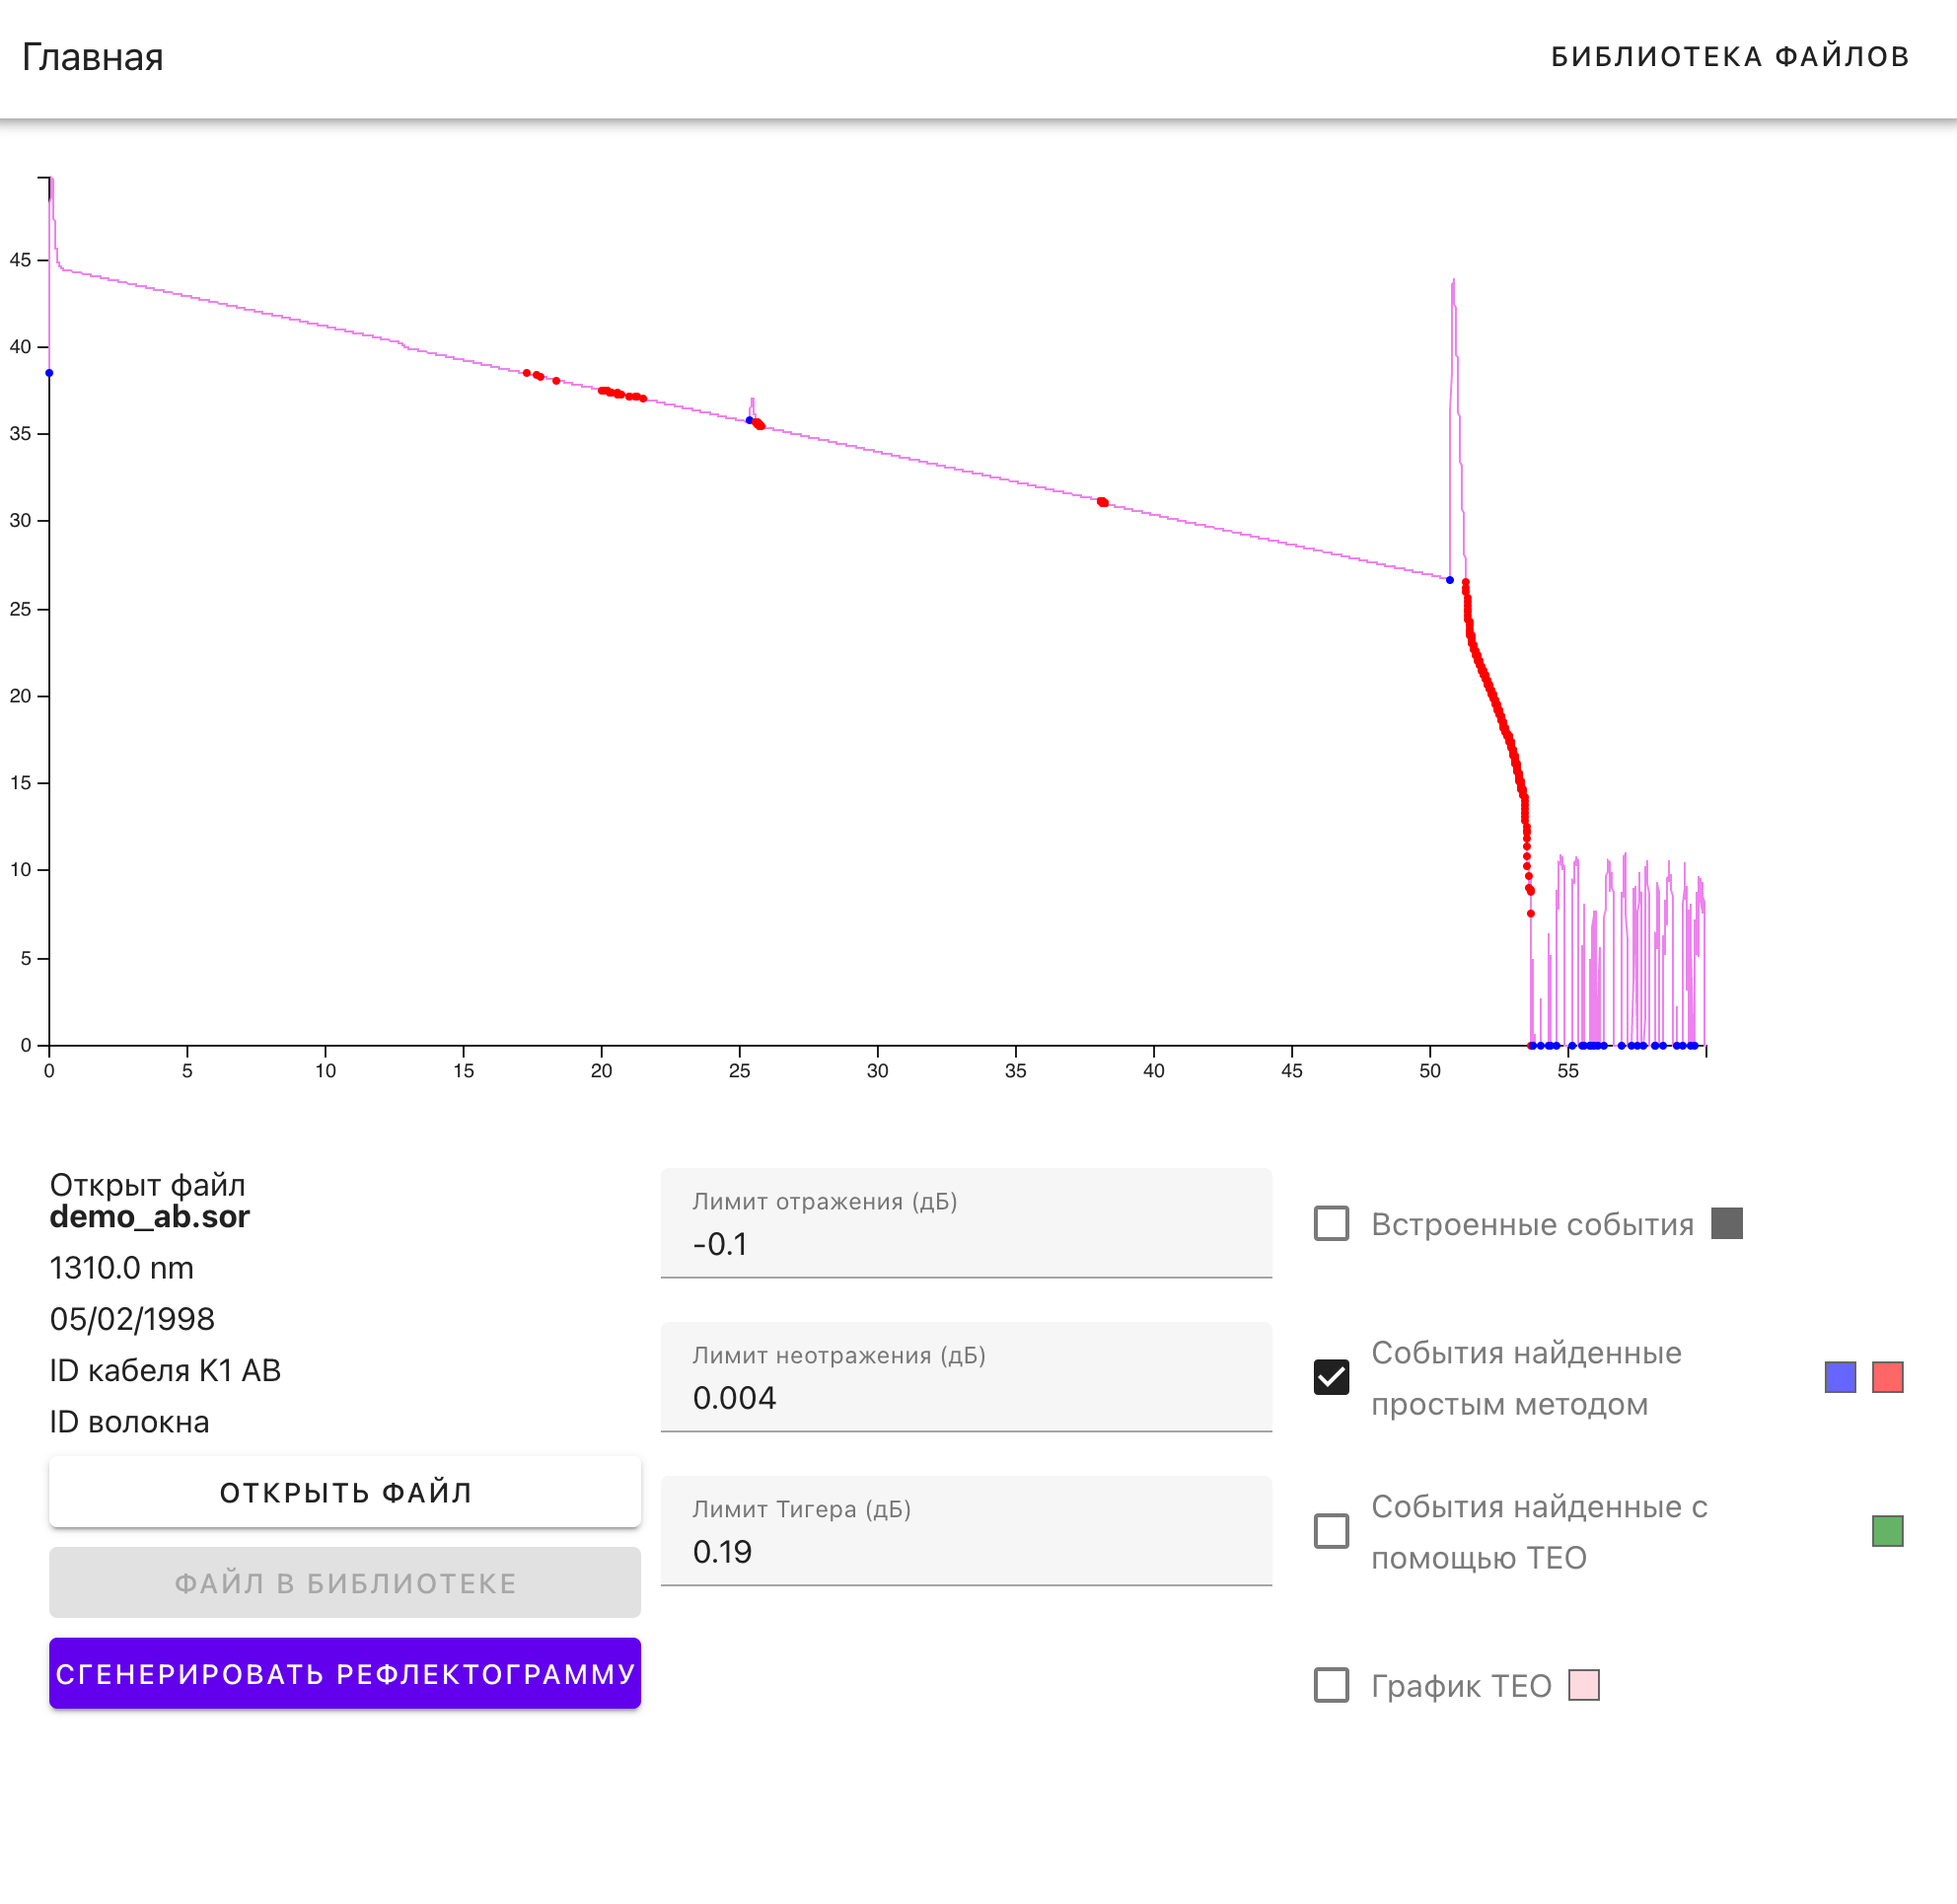
\includegraphics[width=0.65\textwidth]{naive_events}}}
  \caption{События найденные простым алгоритмом}
  \label{ris:naive_events}
\end{figure}

\begin{figure}[H]
  \center{\frame{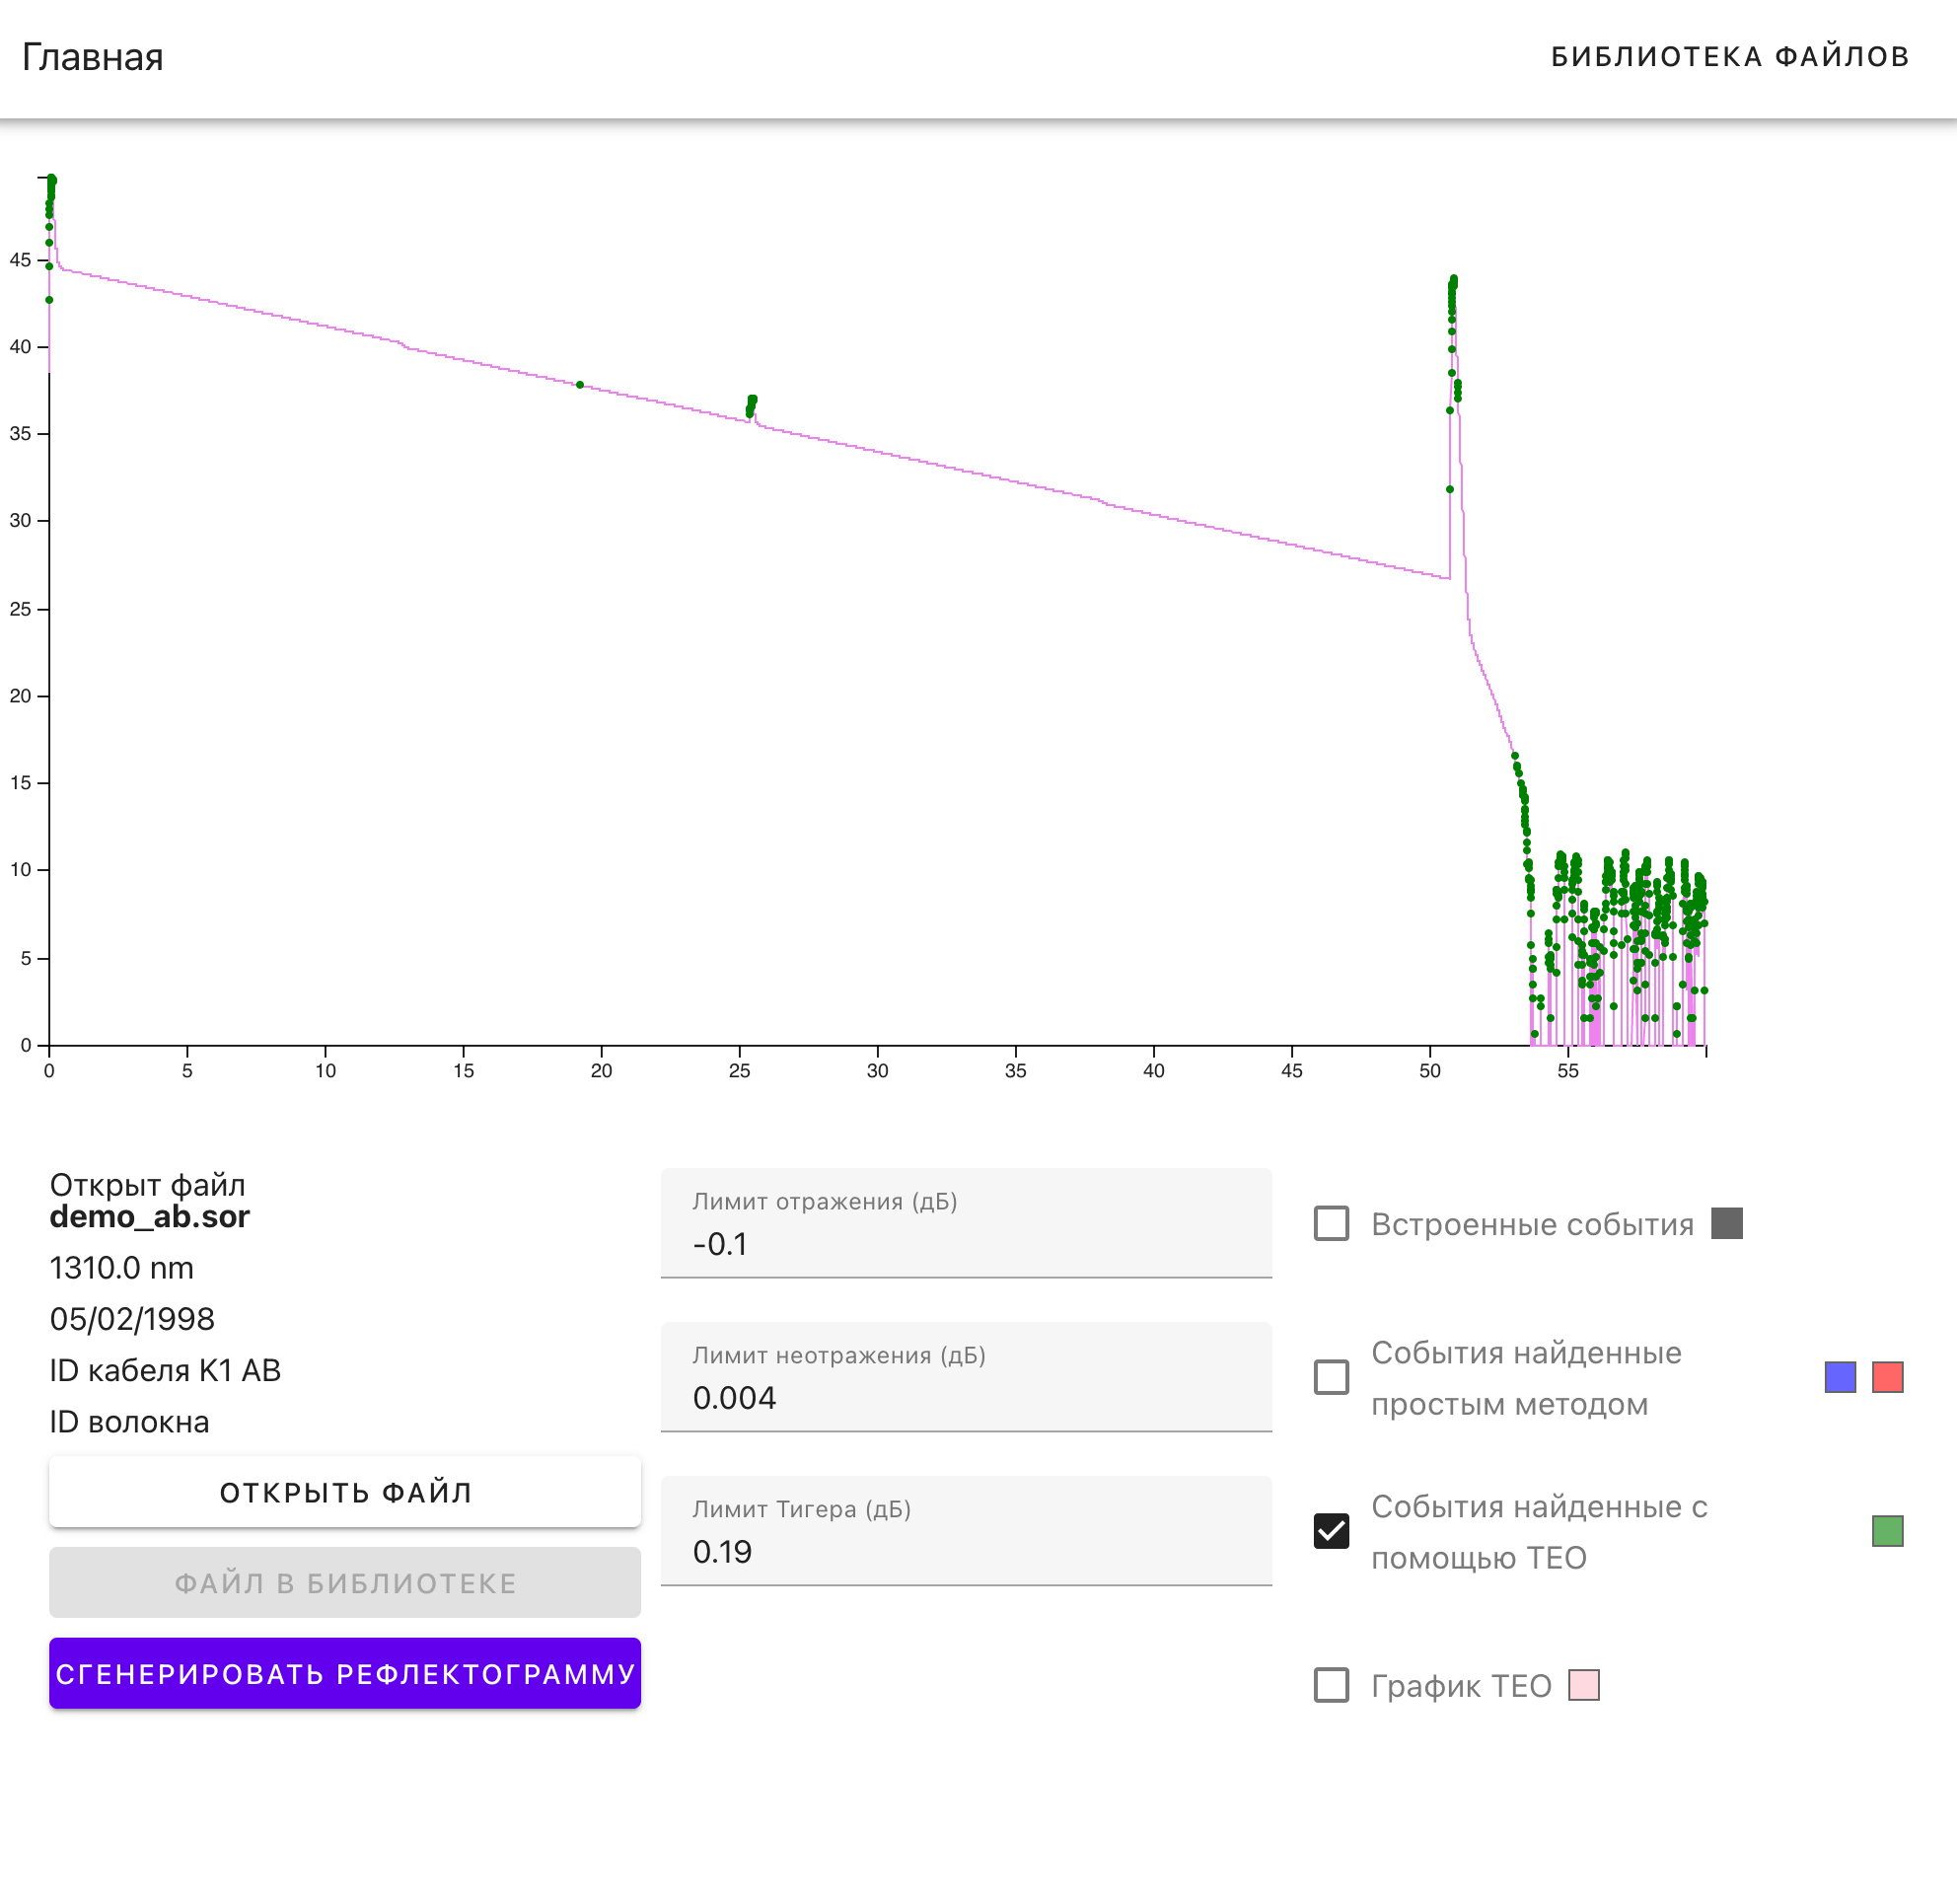
\includegraphics[width=0.65\textwidth]{teo_events}}}
  \caption{События найденные алгоритмом на основе \acrshort{teo}}
  \label{ris:teo_events}
\end{figure}

\begin{figure}[H]
  \center{\frame{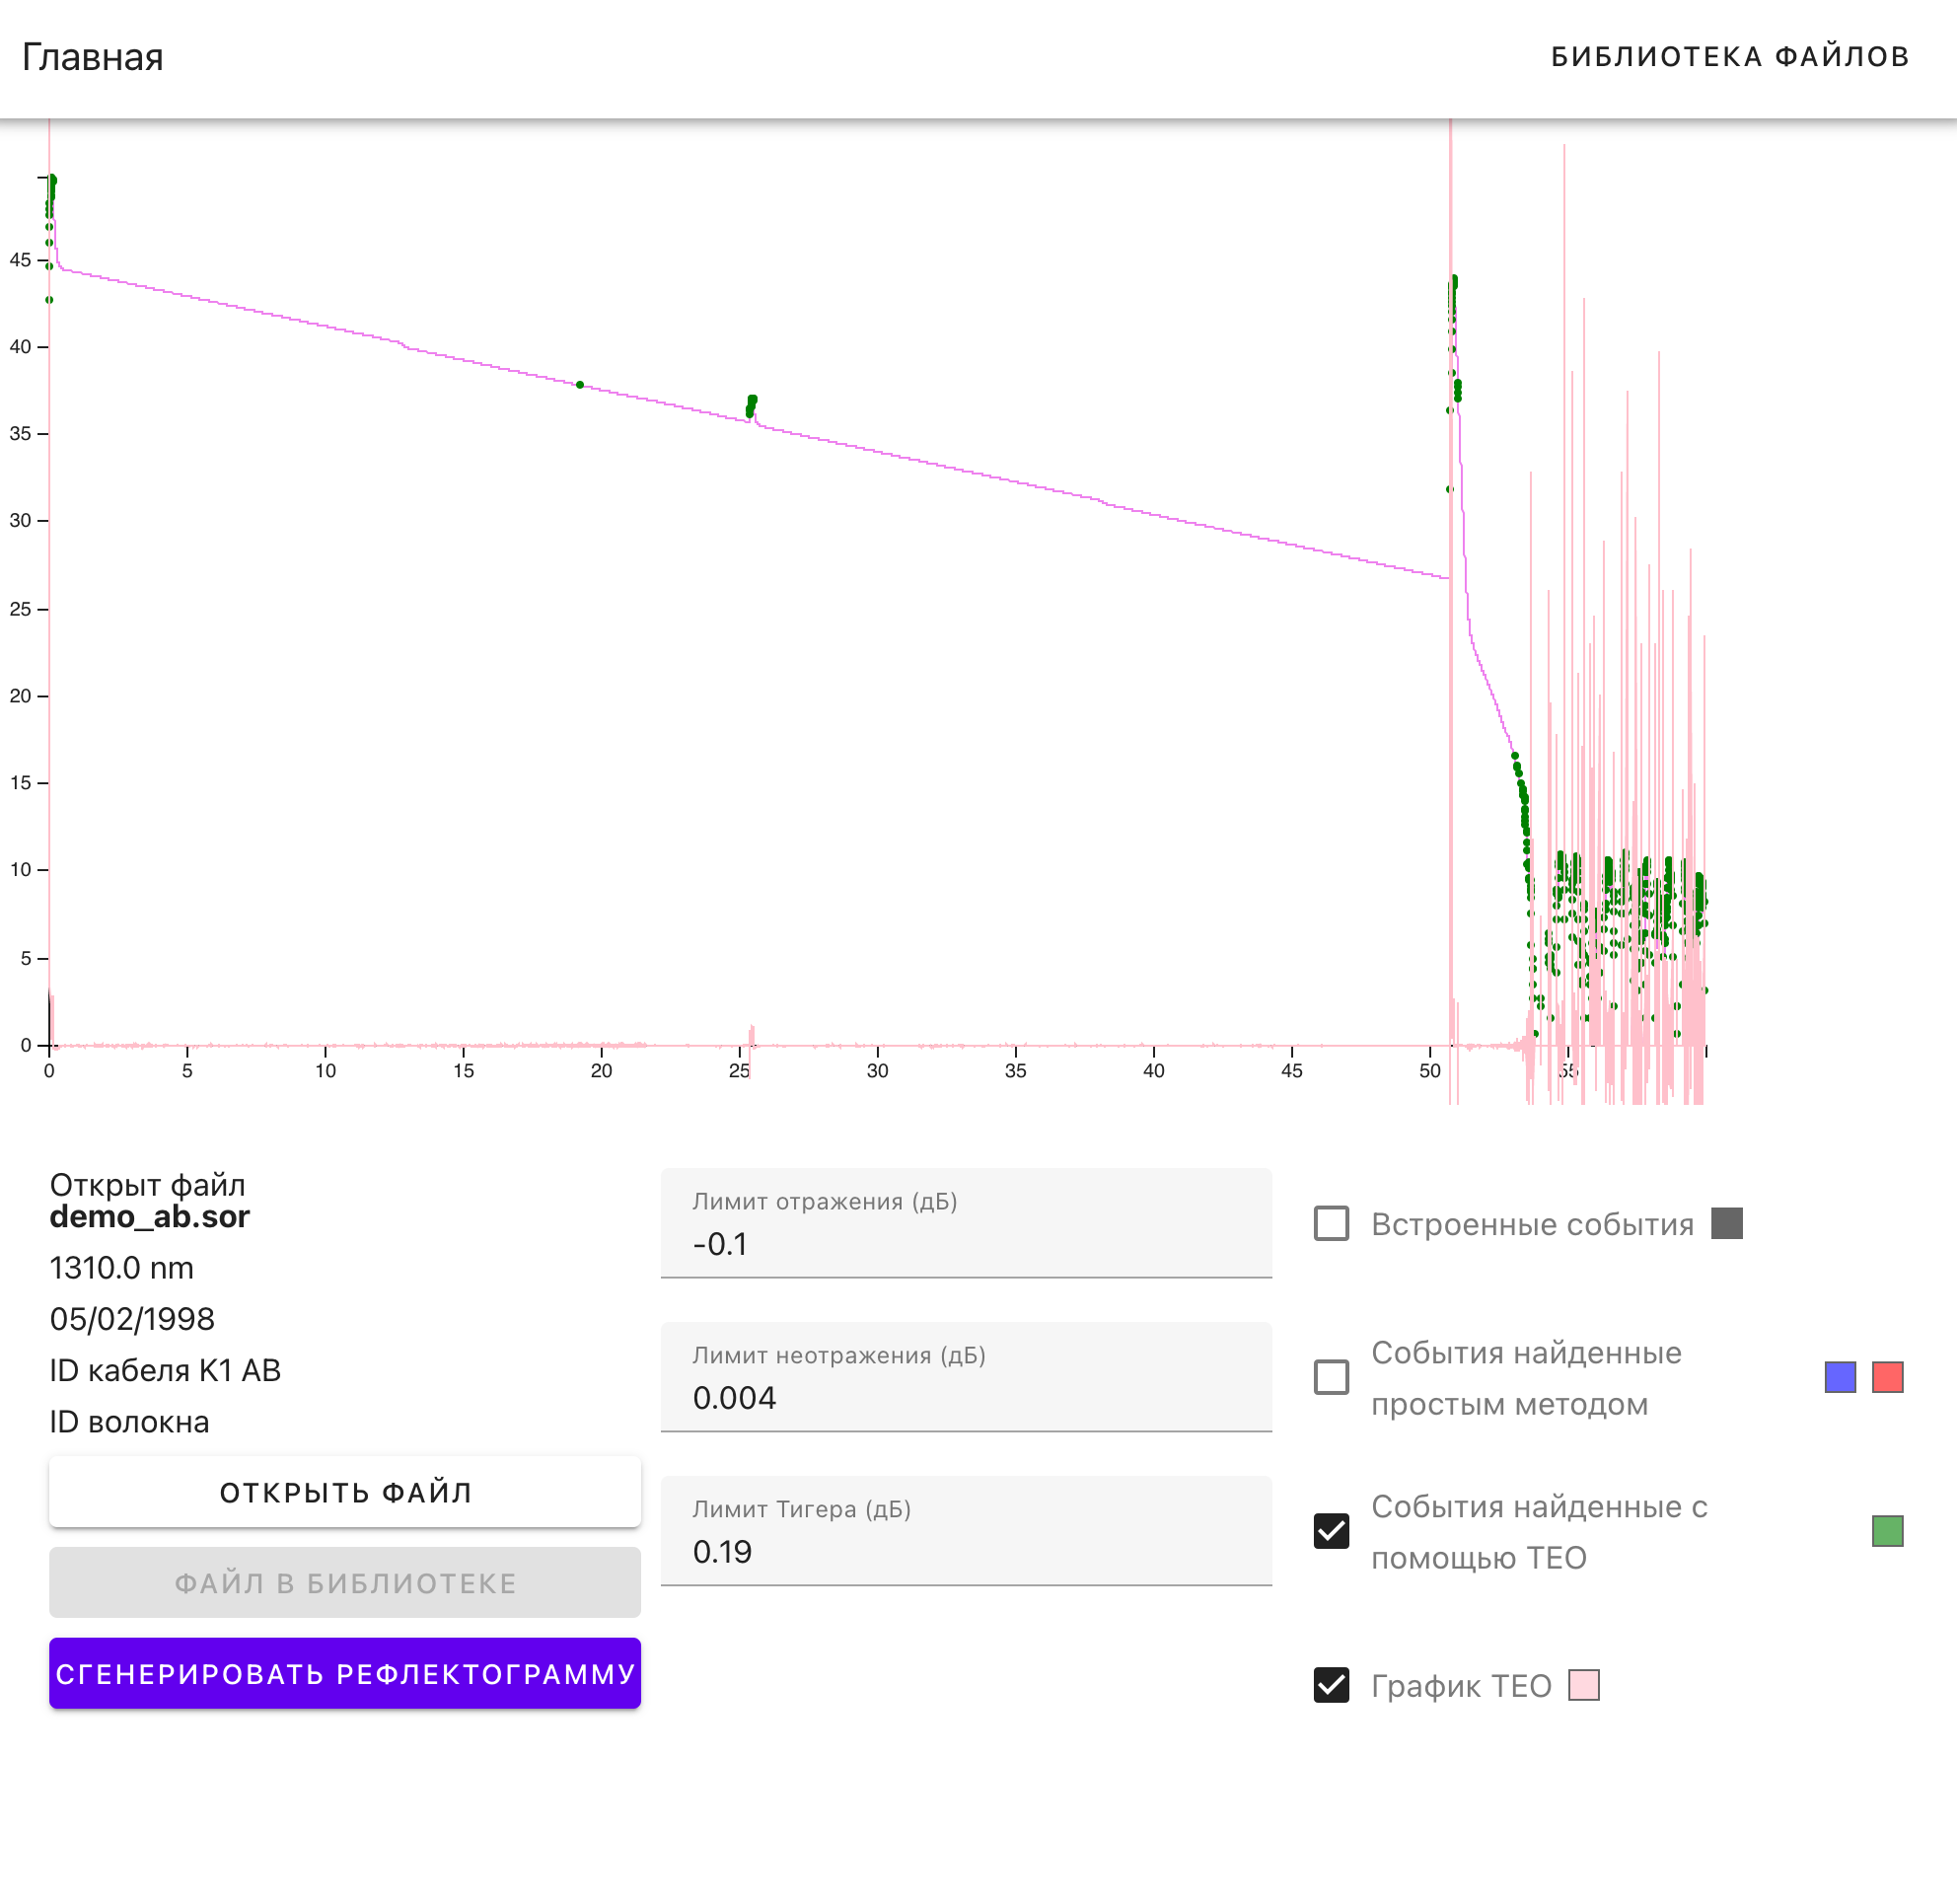
\includegraphics[width=0.65\textwidth]{teo_events_and_values}}}
  \caption{События найденные алгоритмом на основе \acrshort{teo} и график значений \acrshort{teo}}
  \label{ris:teo_events_and_values}
\end{figure}

\begin{figure}[H]
  \center{\frame{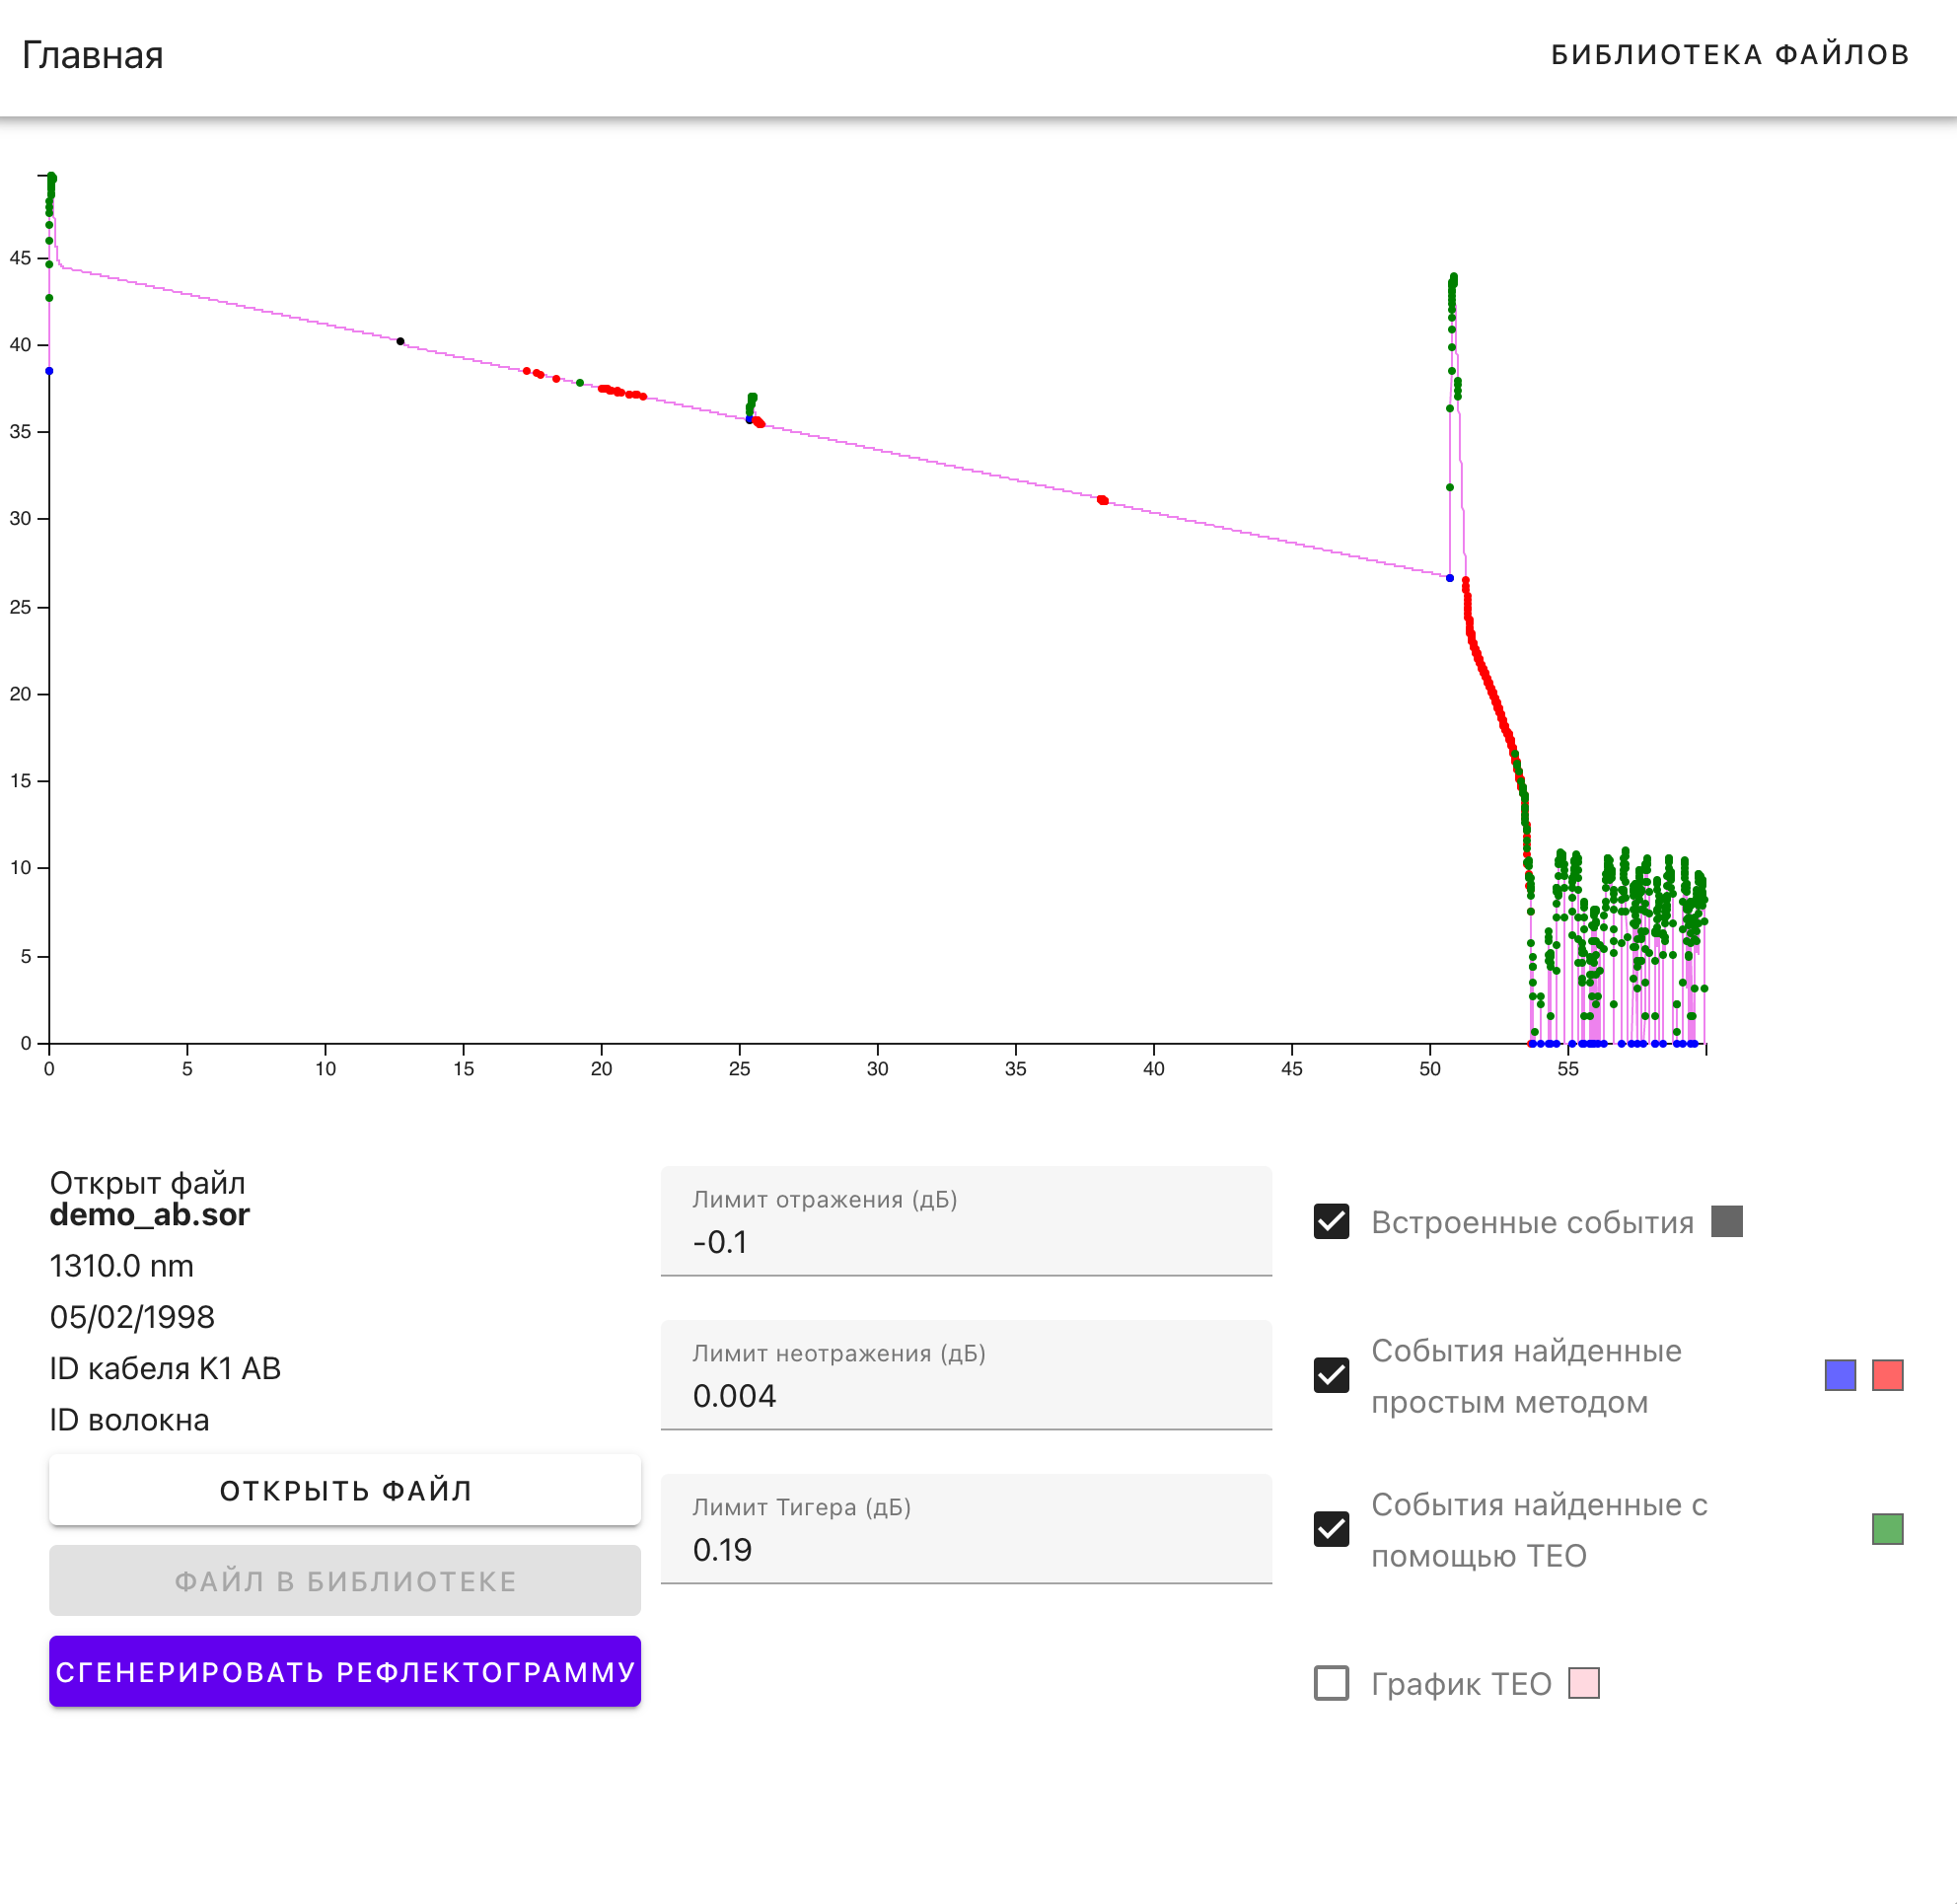
\includegraphics[width=0.65\textwidth]{all_events}}}
  \caption{Все найденные события}
  \label{ris:all_events}
\end{figure}

\subsection{Функция <<Встроенная библиотека>>}

\begin{figure}[H]
  \center{\frame{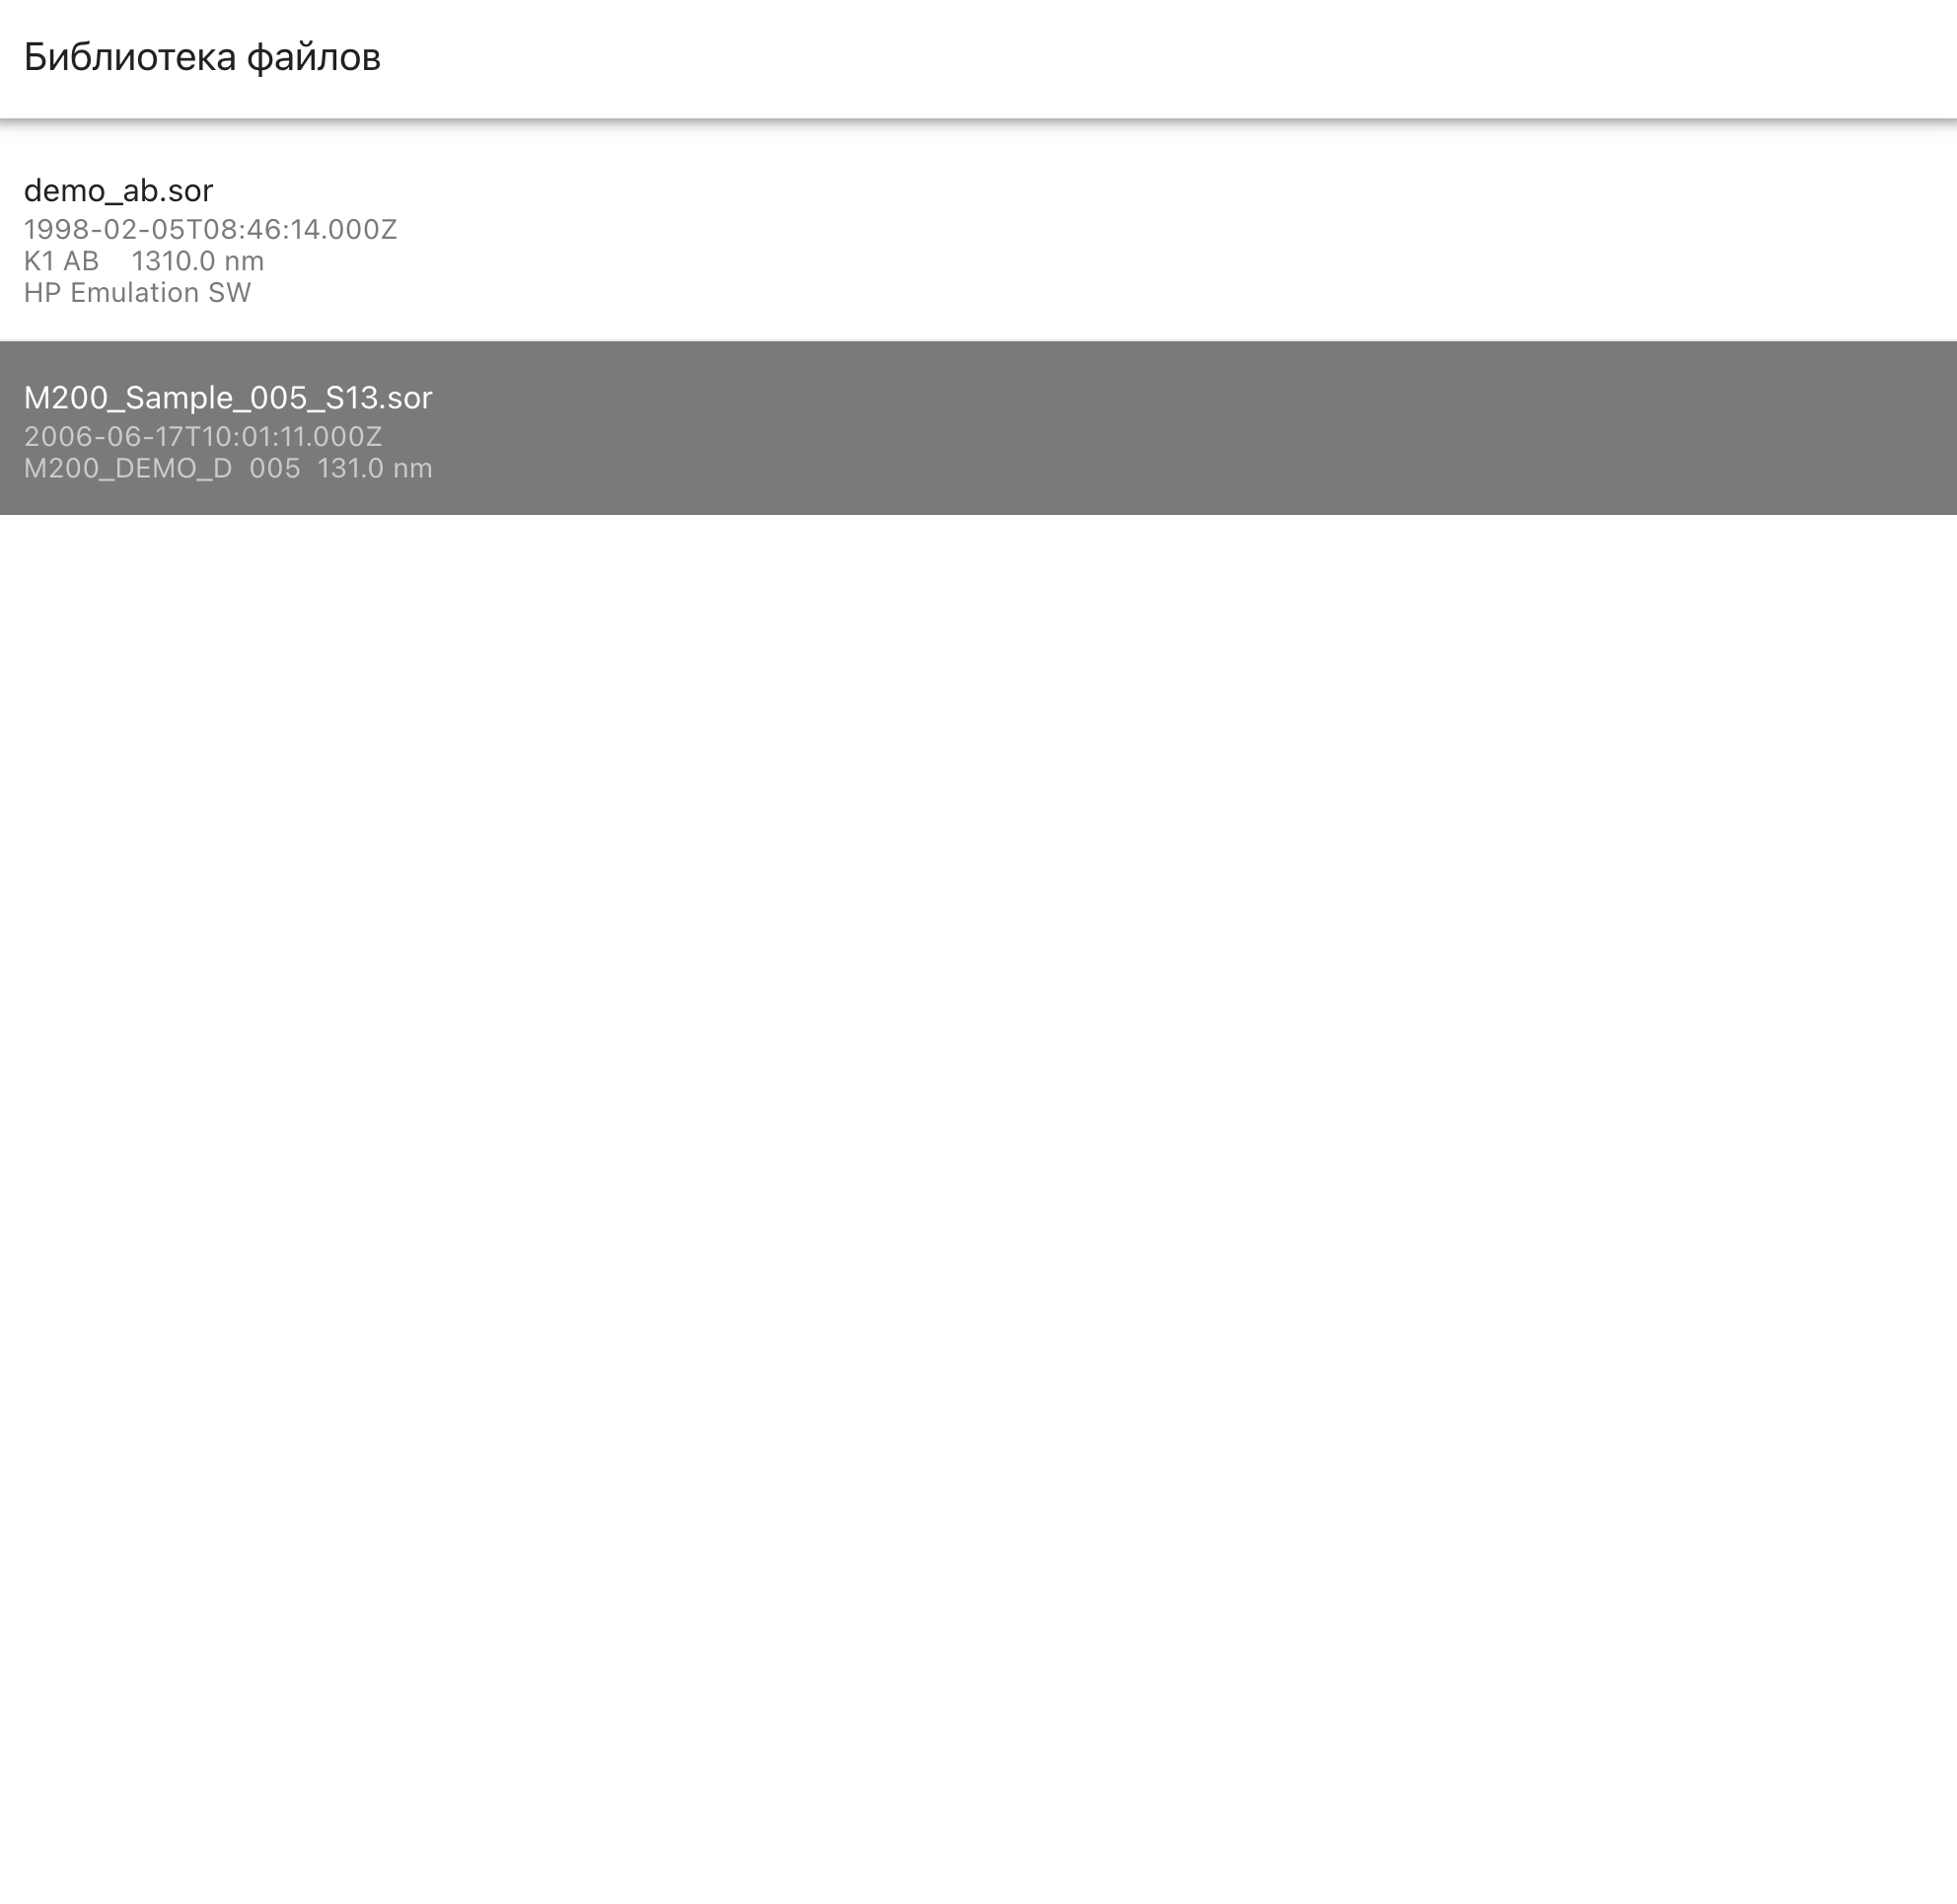
\includegraphics[width=0.65\textwidth]{library}}}
  \caption{Библиотека рефлектограмм}
  \label{ris:library}
\end{figure}

\subsection{Функция <<Редактирование рефлектограммы>>}

\begin{figure}[H]
  \center{\frame{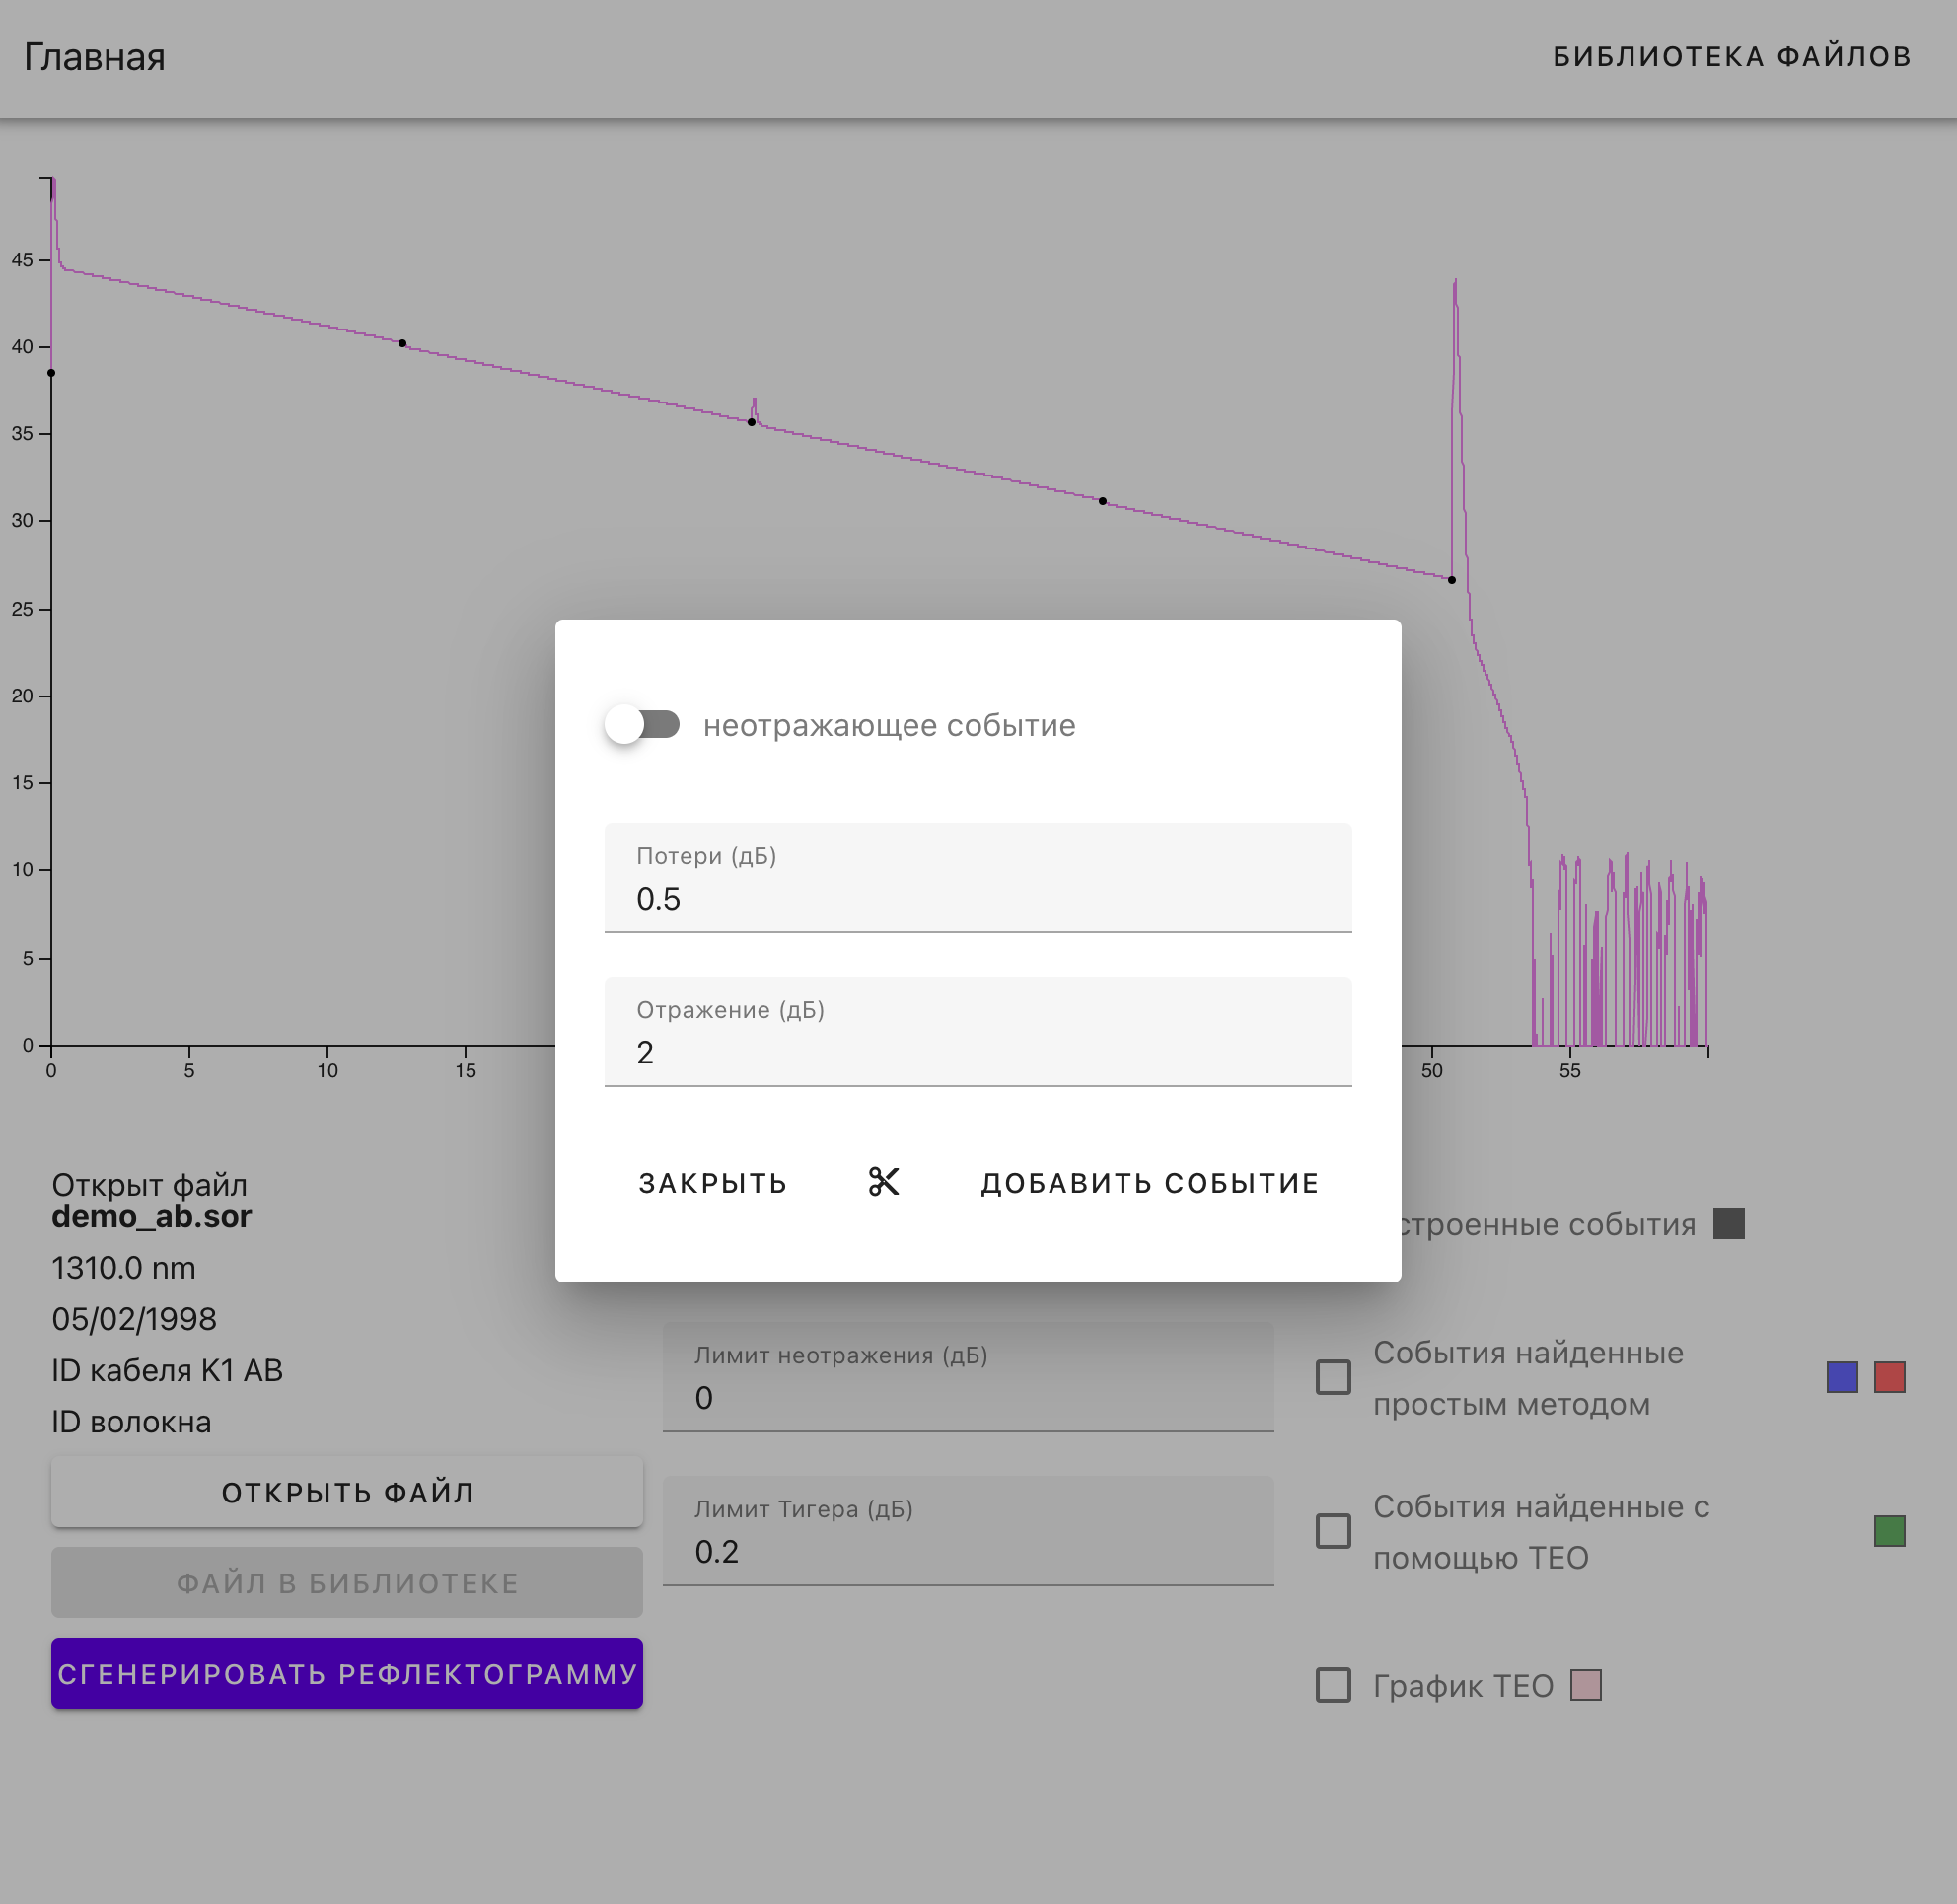
\includegraphics[width=0.65\textwidth]{edit_modal}}}
  \caption{\Gls{модальное окно} редактирования}
  \label{ris:edit_modal}
\end{figure}

\begin{figure}[H]
  \center{\frame{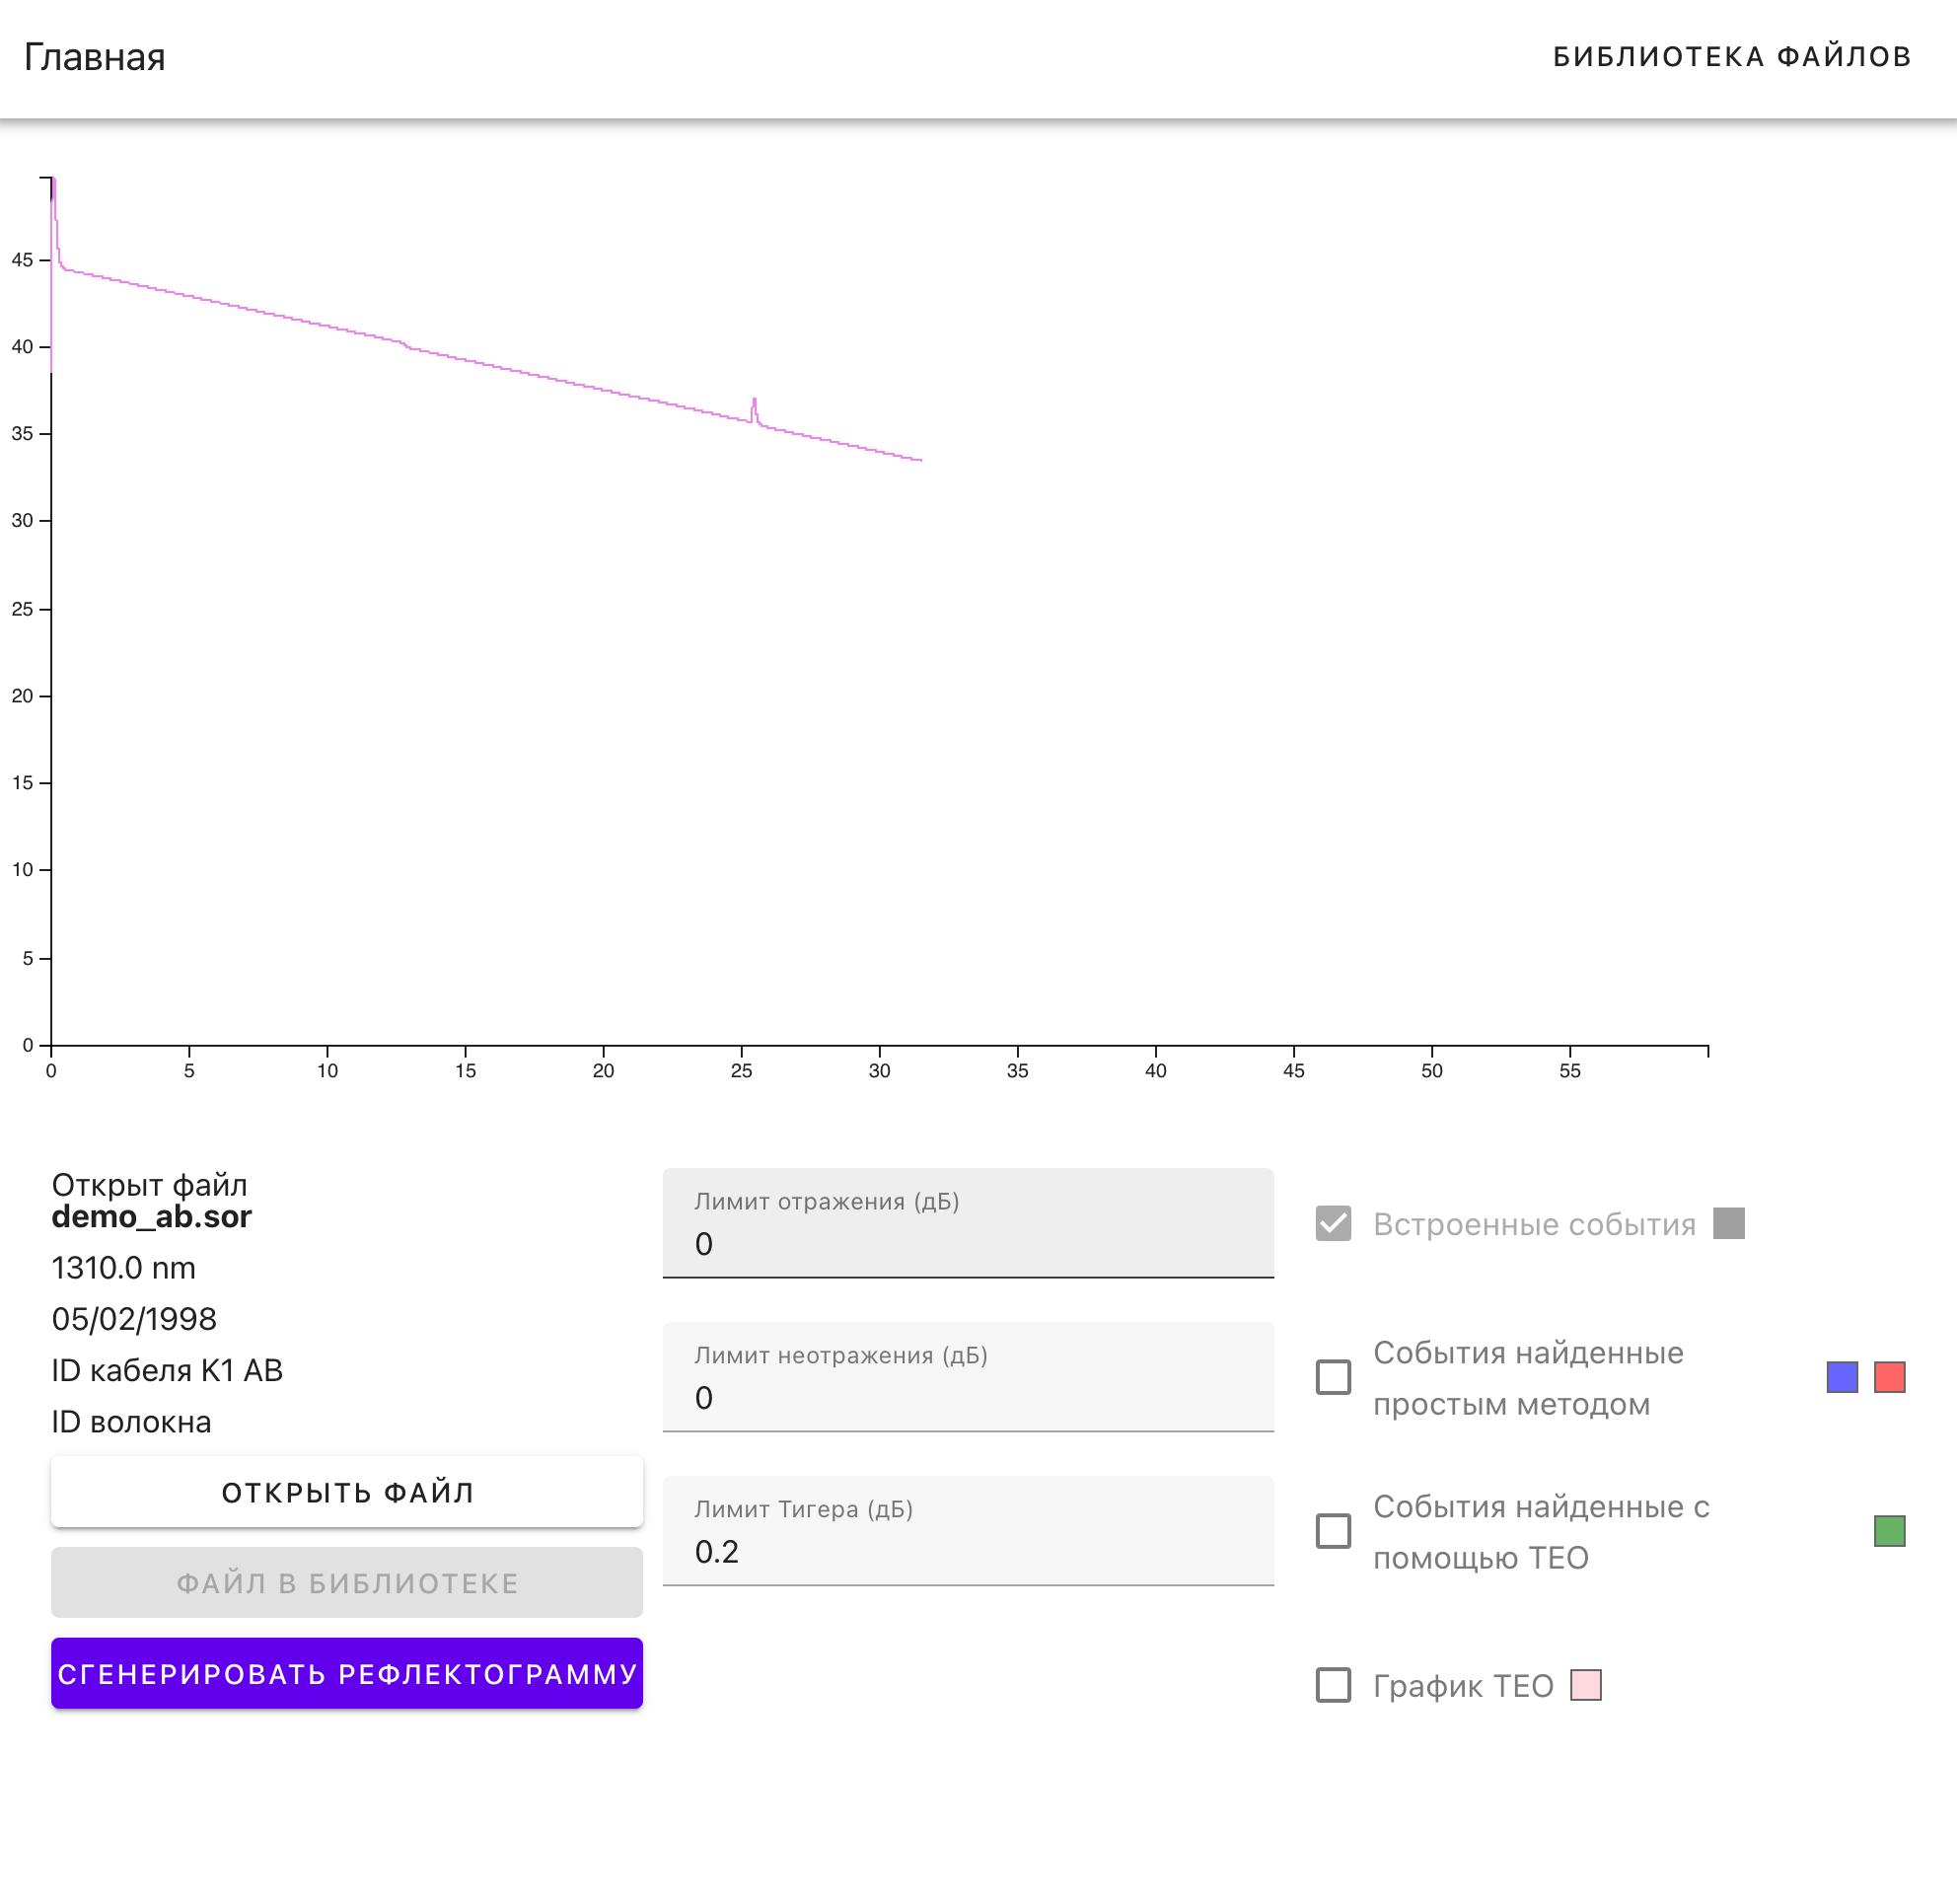
\includegraphics[width=0.65\textwidth]{cut_result}}}
  \caption{Результат выполнения действия <<Обрезка рефлектограммы>>}
  \label{ris:cut_result}
\end{figure}

\begin{figure}[H]
  \center{\frame{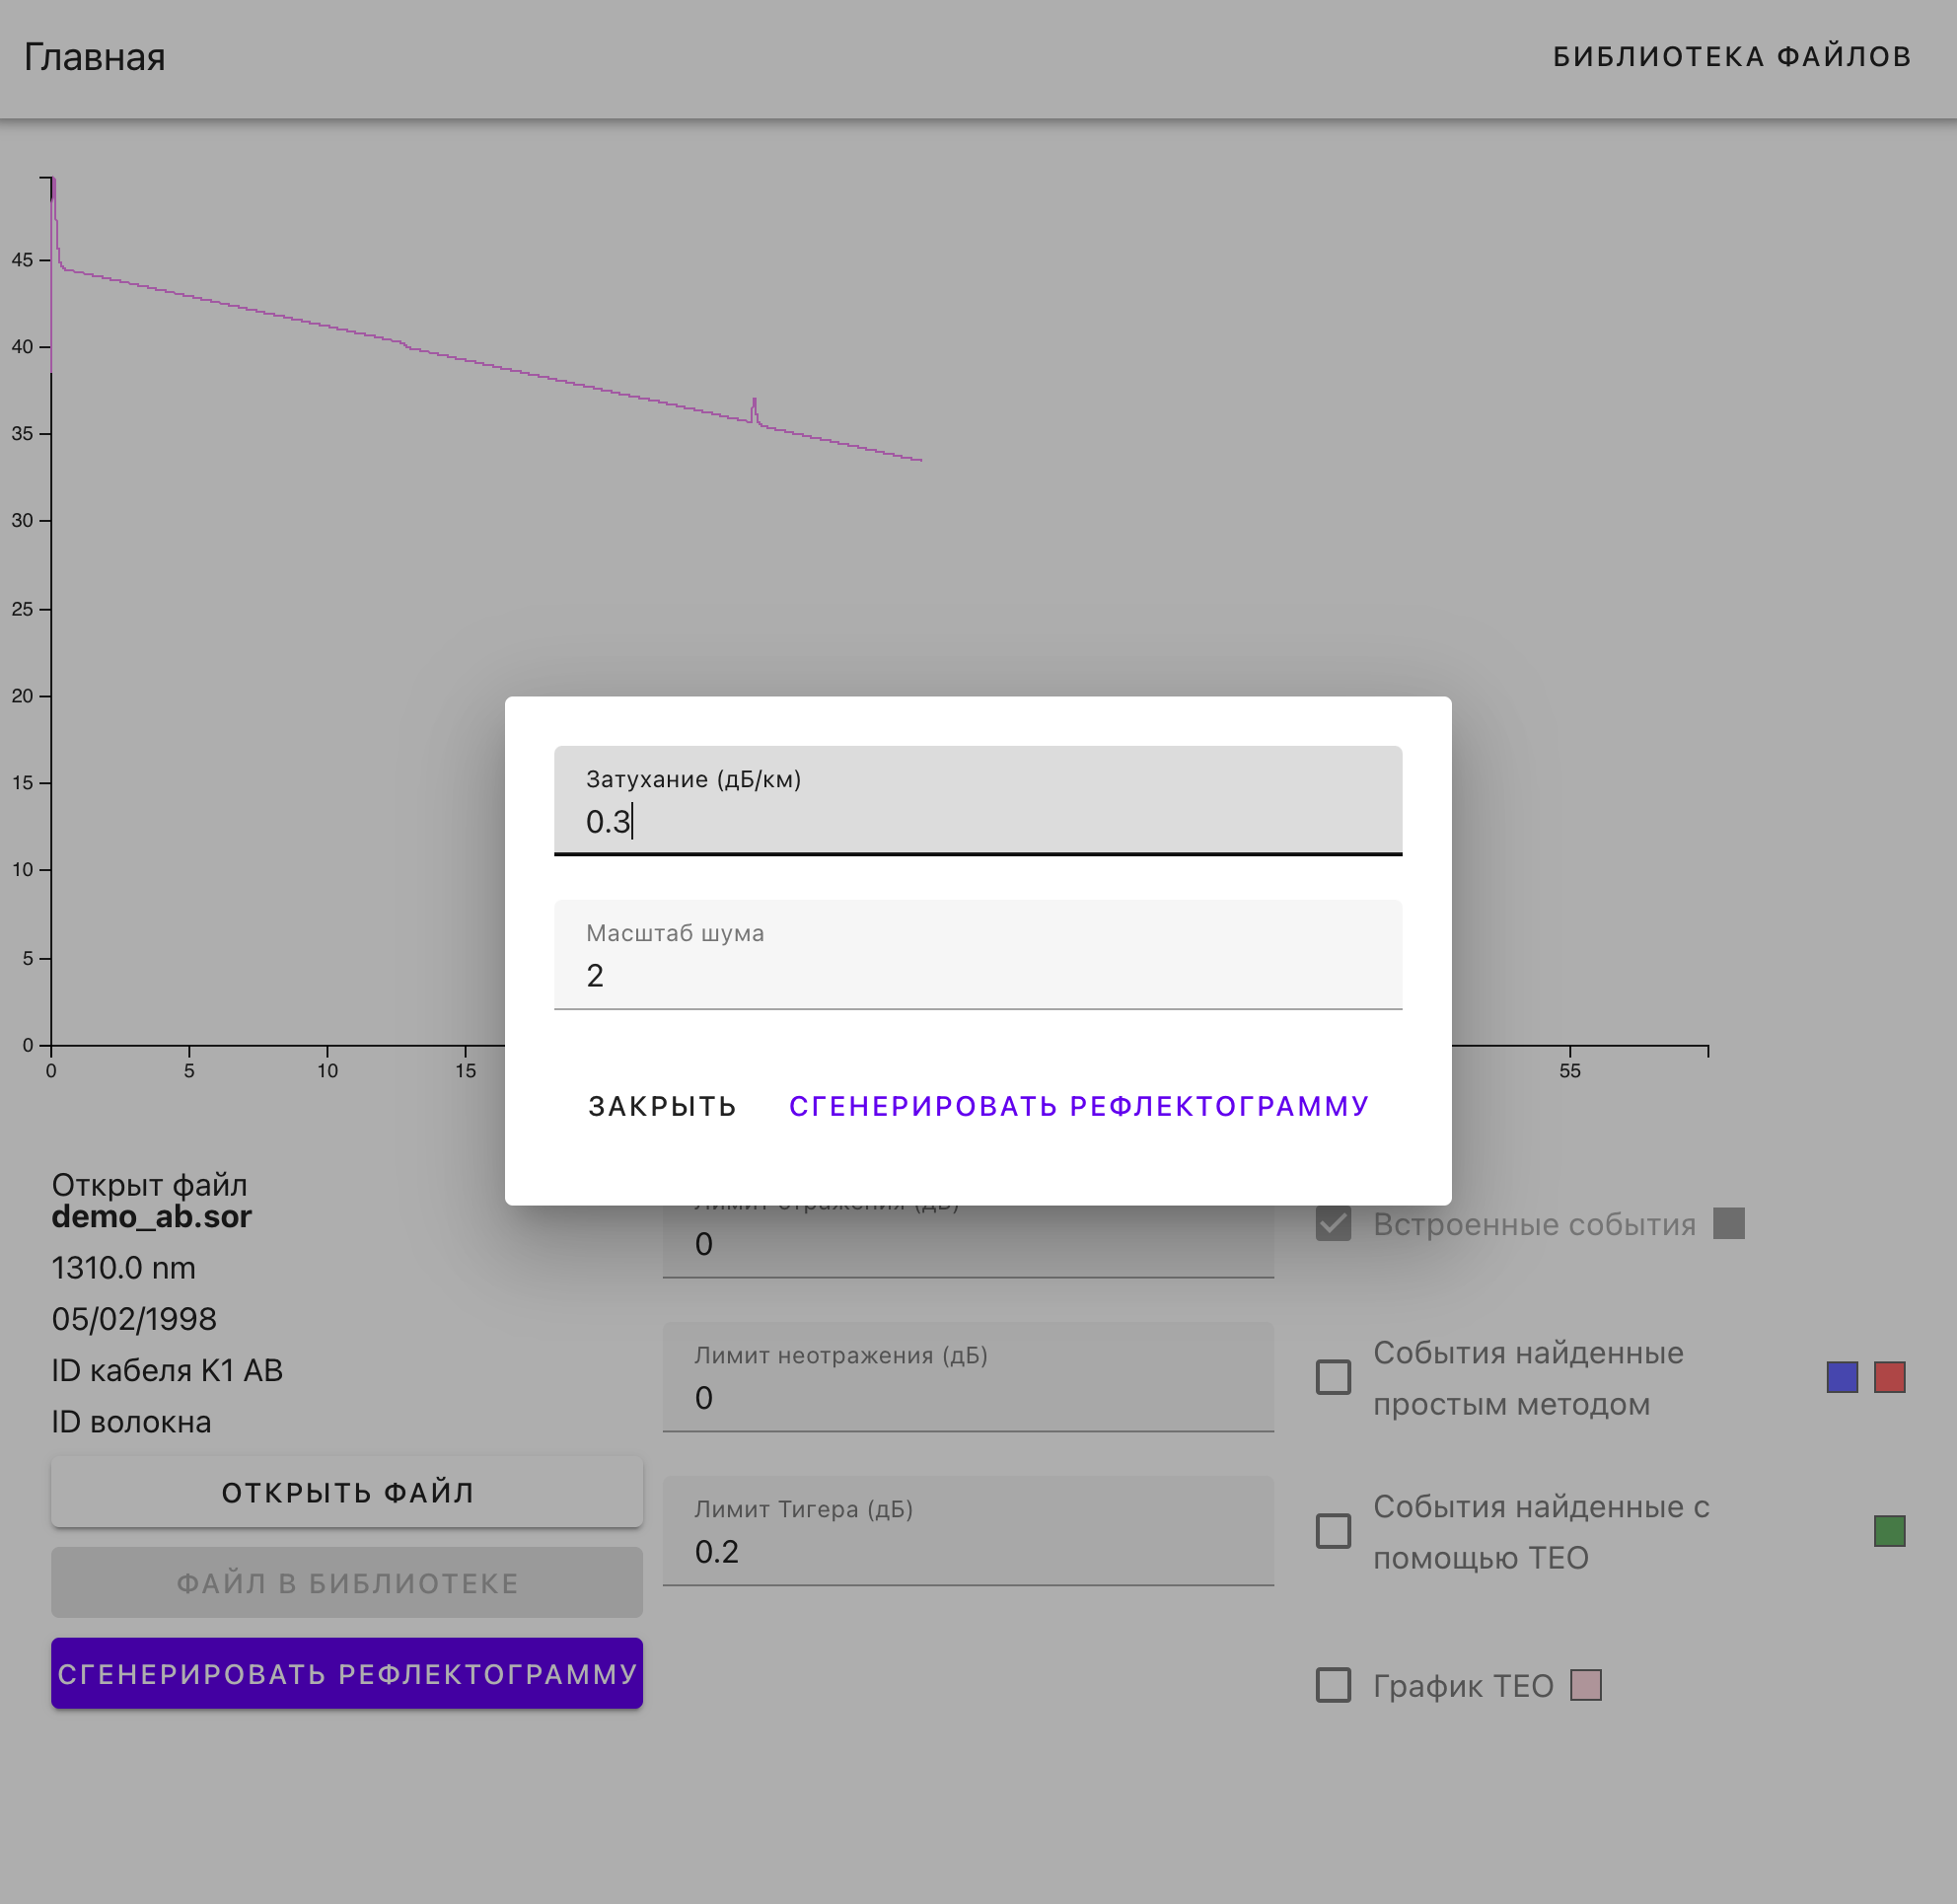
\includegraphics[width=0.65\textwidth]{generate}}}
  \caption{\Gls{модальное окно} <<Сгенерировать рефлектограммму>>}
  \label{ris:generate}
\end{figure}

\begin{figure}[H]
  \center{\frame{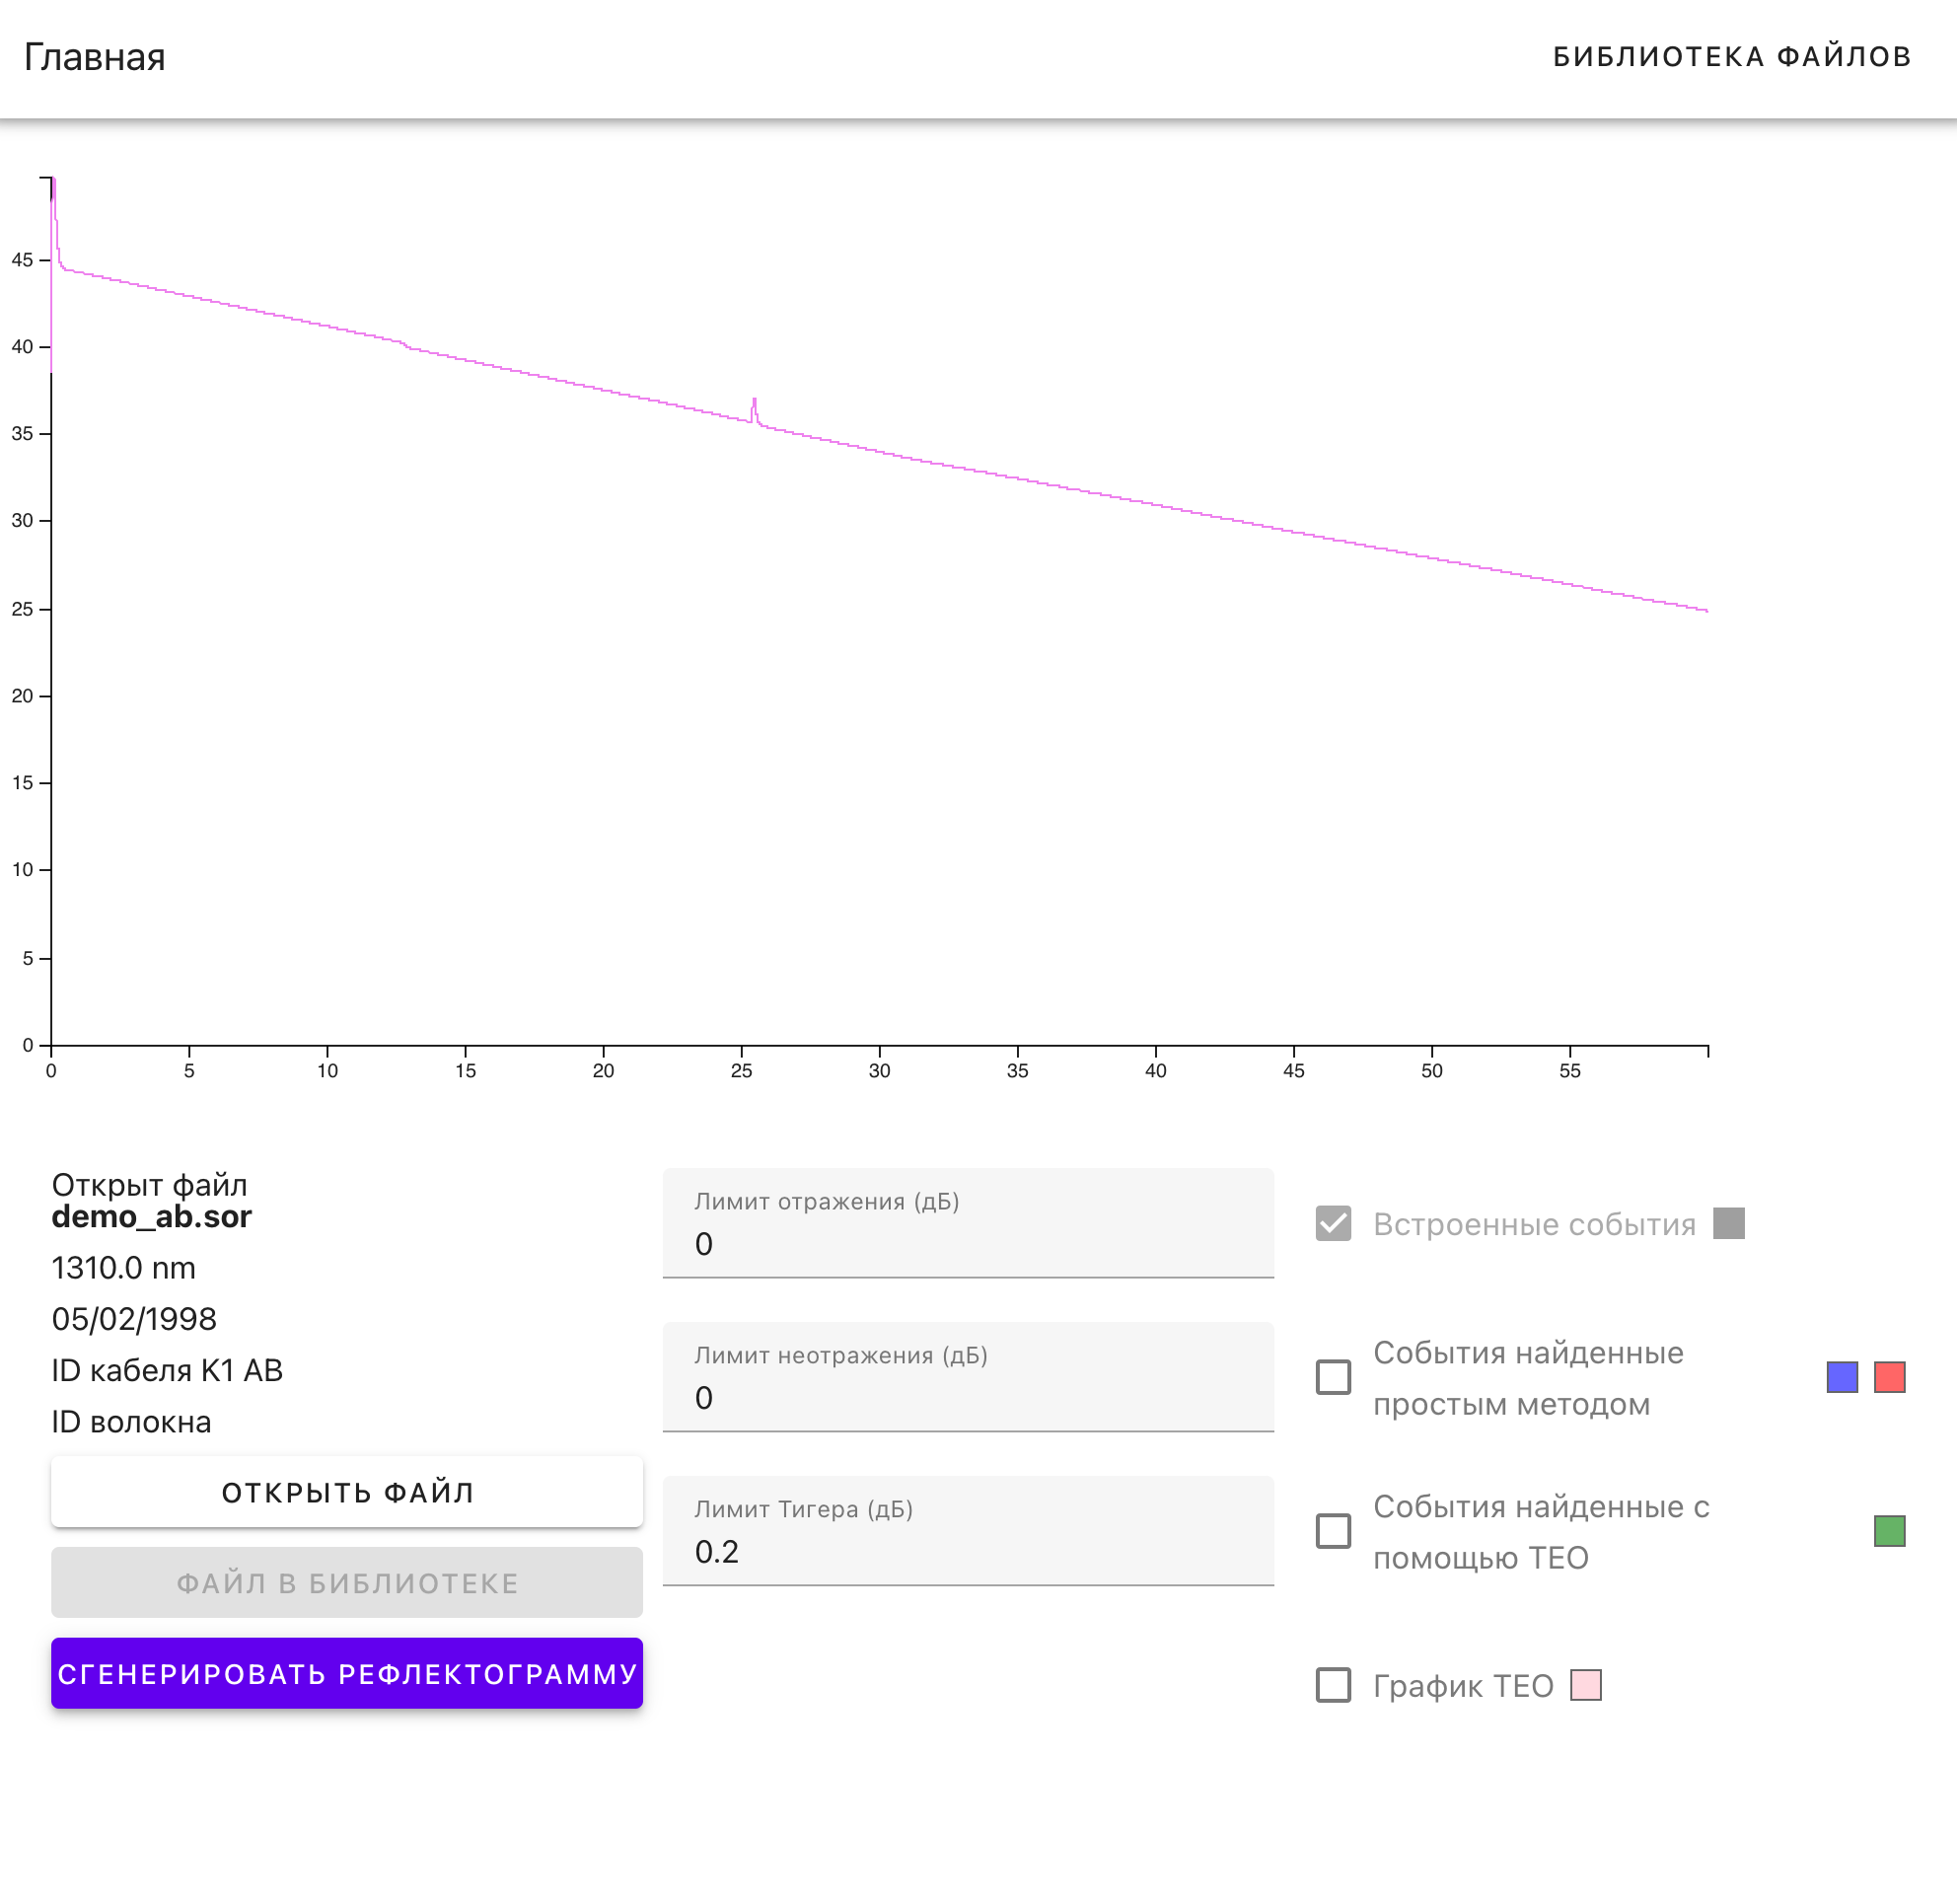
\includegraphics[width=0.65\textwidth]{generate_result}}}
  \caption{Результат выполнения действия <<Сгенерировать рефлектограммму>>}
  \label{ris:generate_result}
\end{figure}

\begin{figure}[H]
  \center{\frame{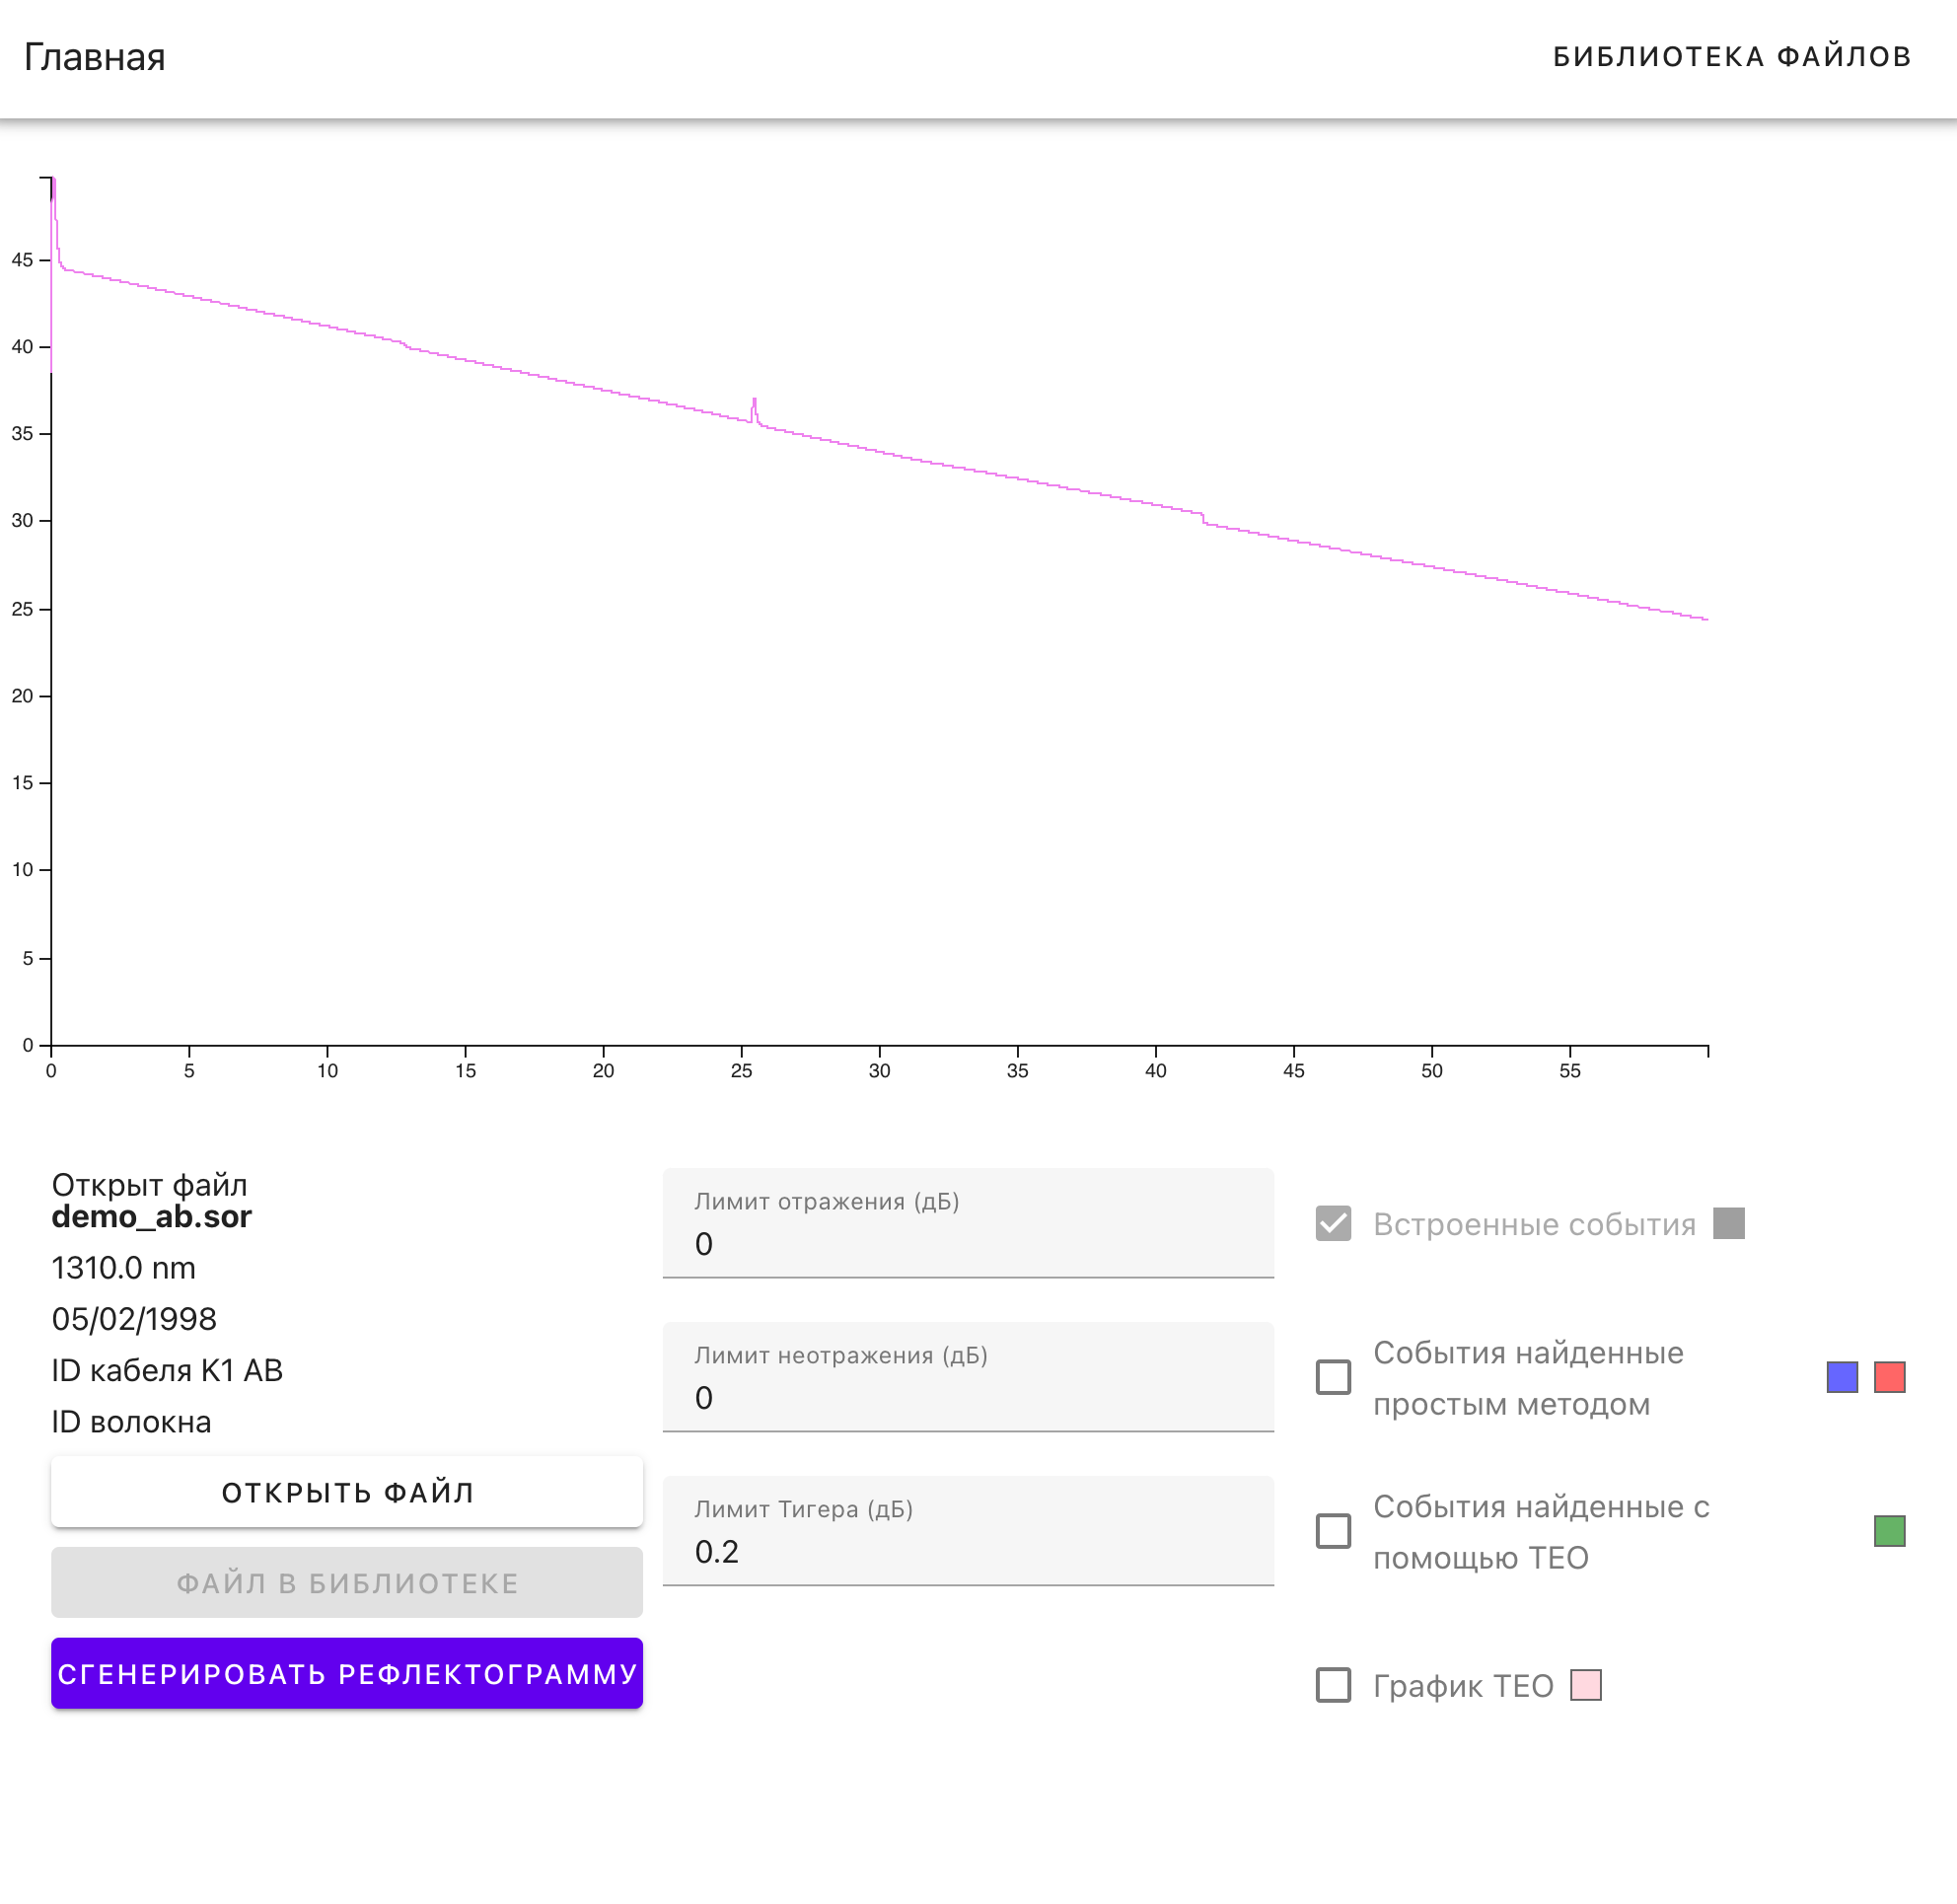
\includegraphics[width=0.65\textwidth]{loss_event_added}}}
  \caption{Результат выполнения действия <<Добавить событие>> с параметром <<Неотражающее событие>>}
  \label{ris:loss_event_added}
\end{figure}

\begin{figure}[H]
  \center{\frame{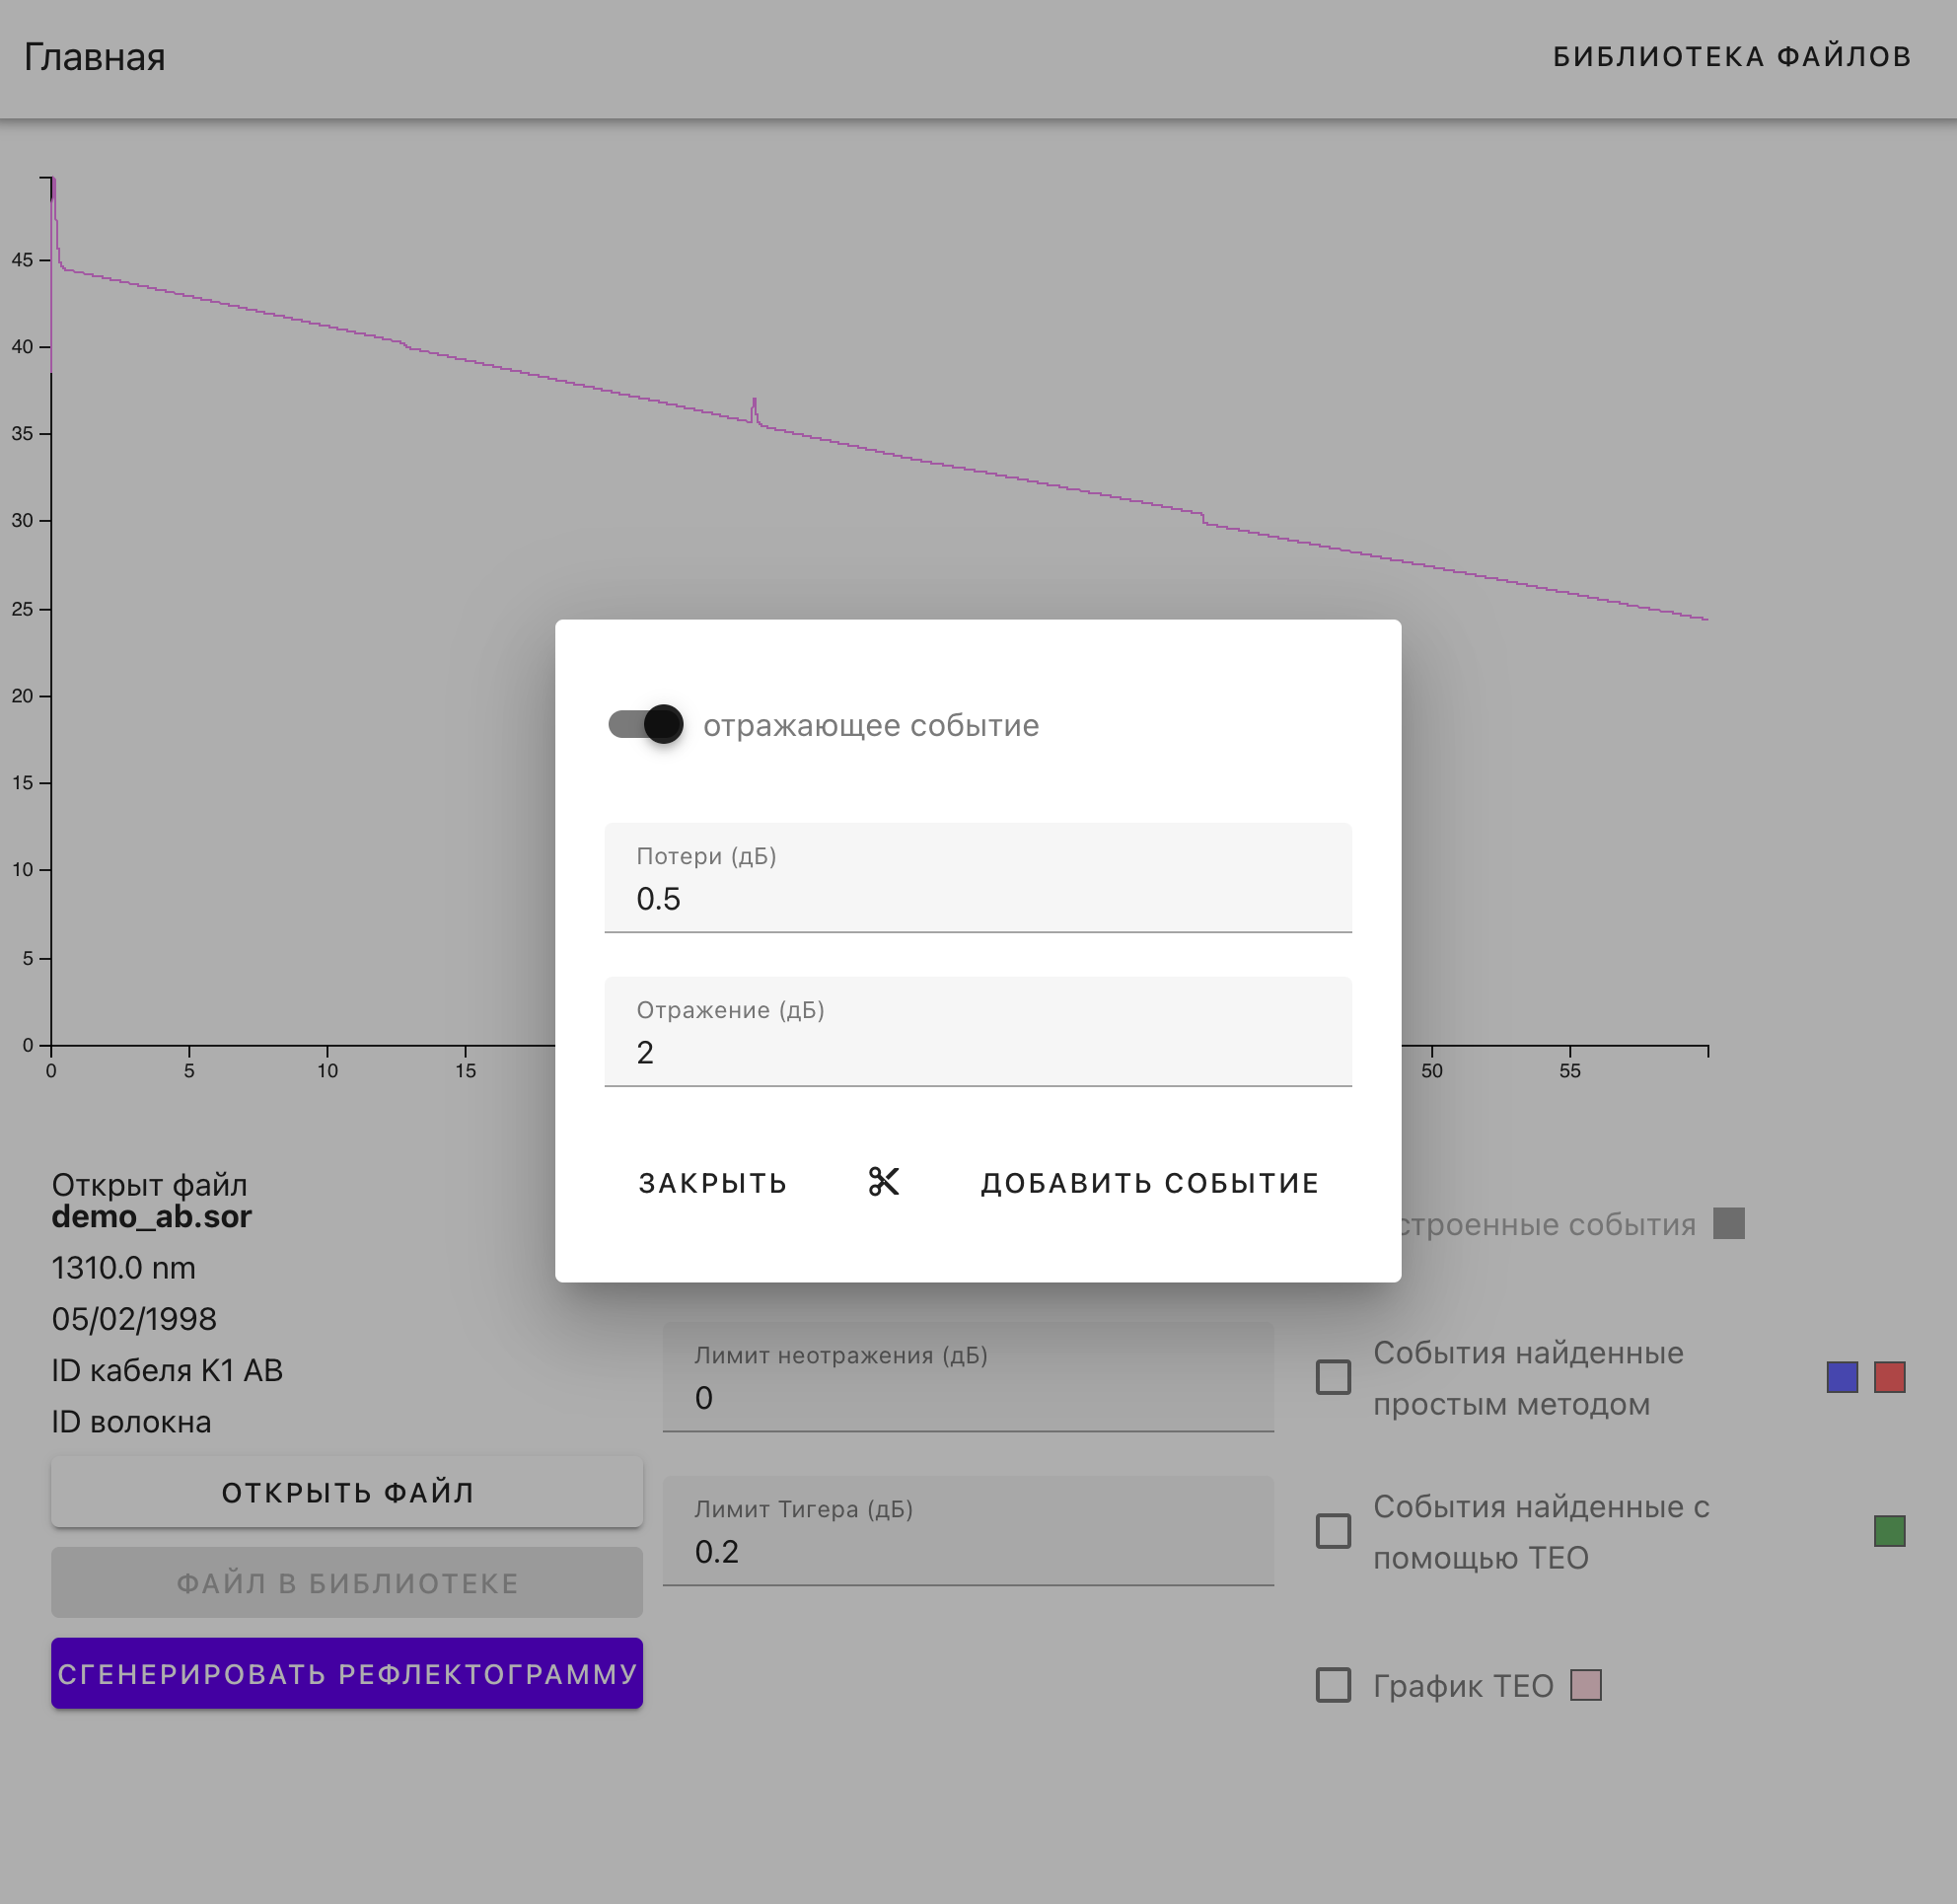
\includegraphics[width=0.65\textwidth]{edit_modal_reflection}}}
  \caption{\Gls{модальное окно} редактирования с селектором в положении <<Отражающее событие>>}
  \label{ris:edit_modal_reflection}
\end{figure}

\begin{figure}[H]
  \center{\frame{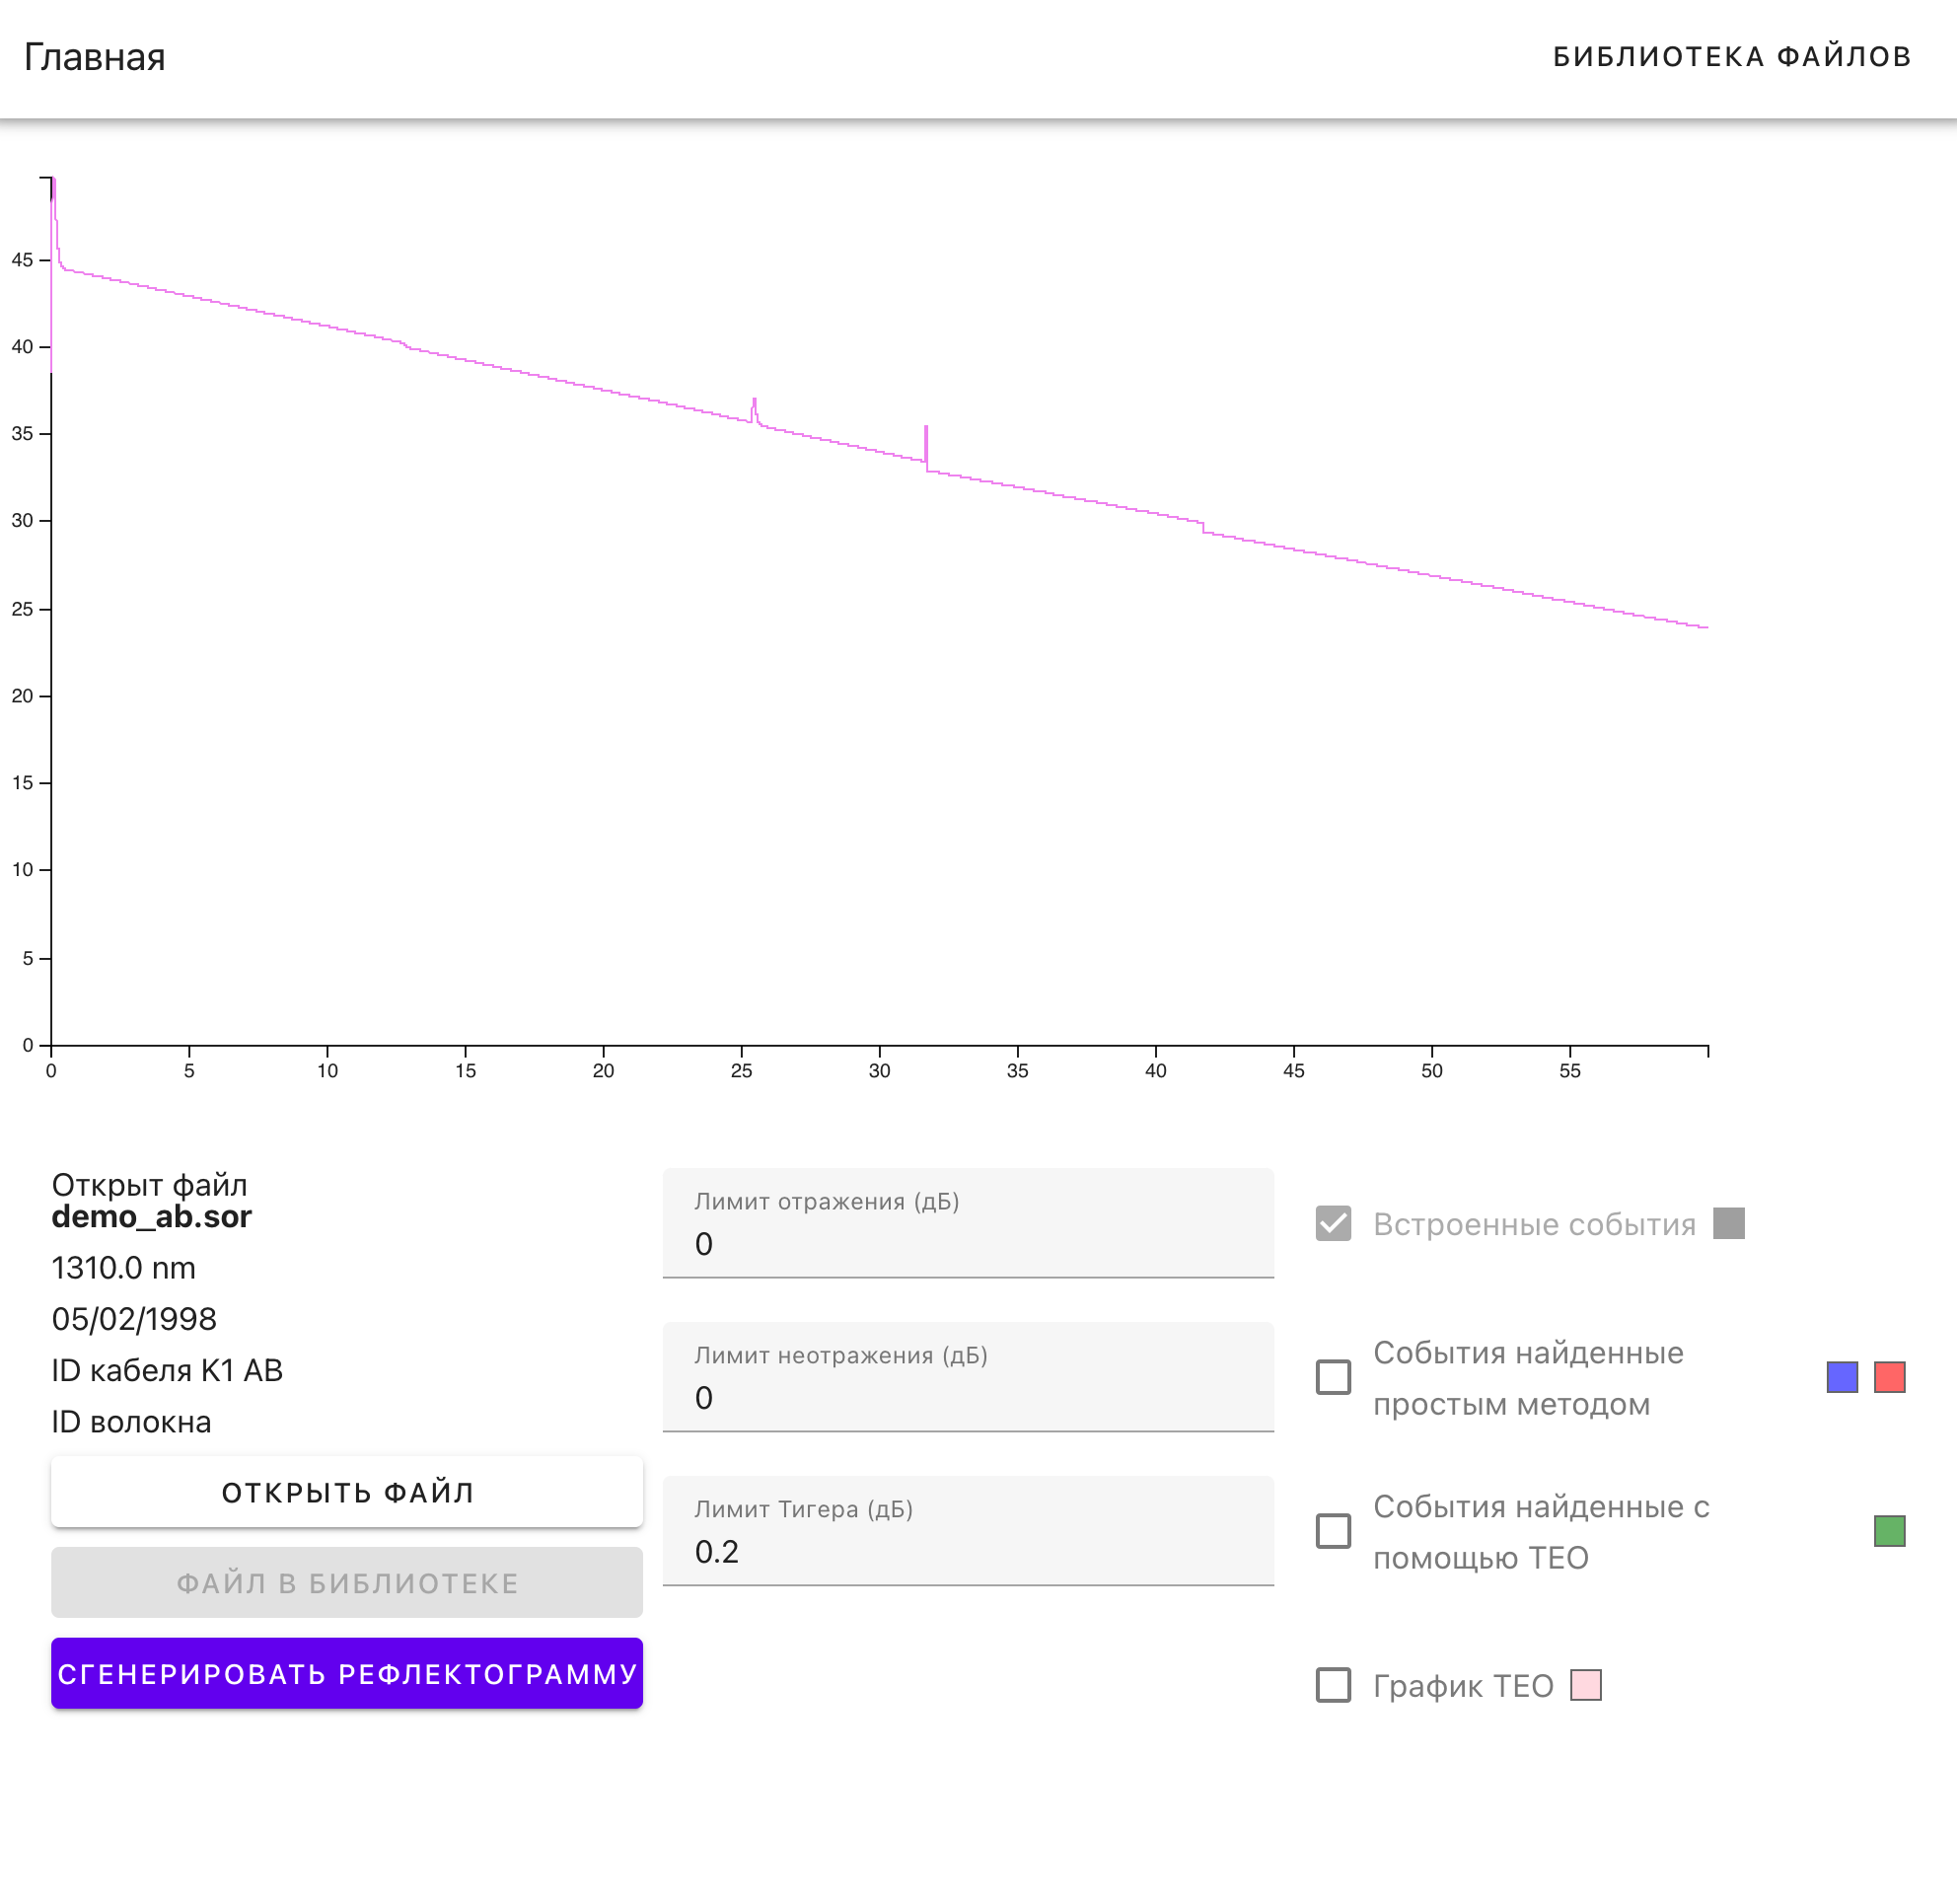
\includegraphics[width=0.65\textwidth]{reflection_event_added}}}
  \caption{Результат выполнения действия <<Добавить событие>> с параметром <<Отражающее событие>>}
  \label{ris:reflection_event_added}
\end{figure}

\begin{figure}[H]
  \center{\frame{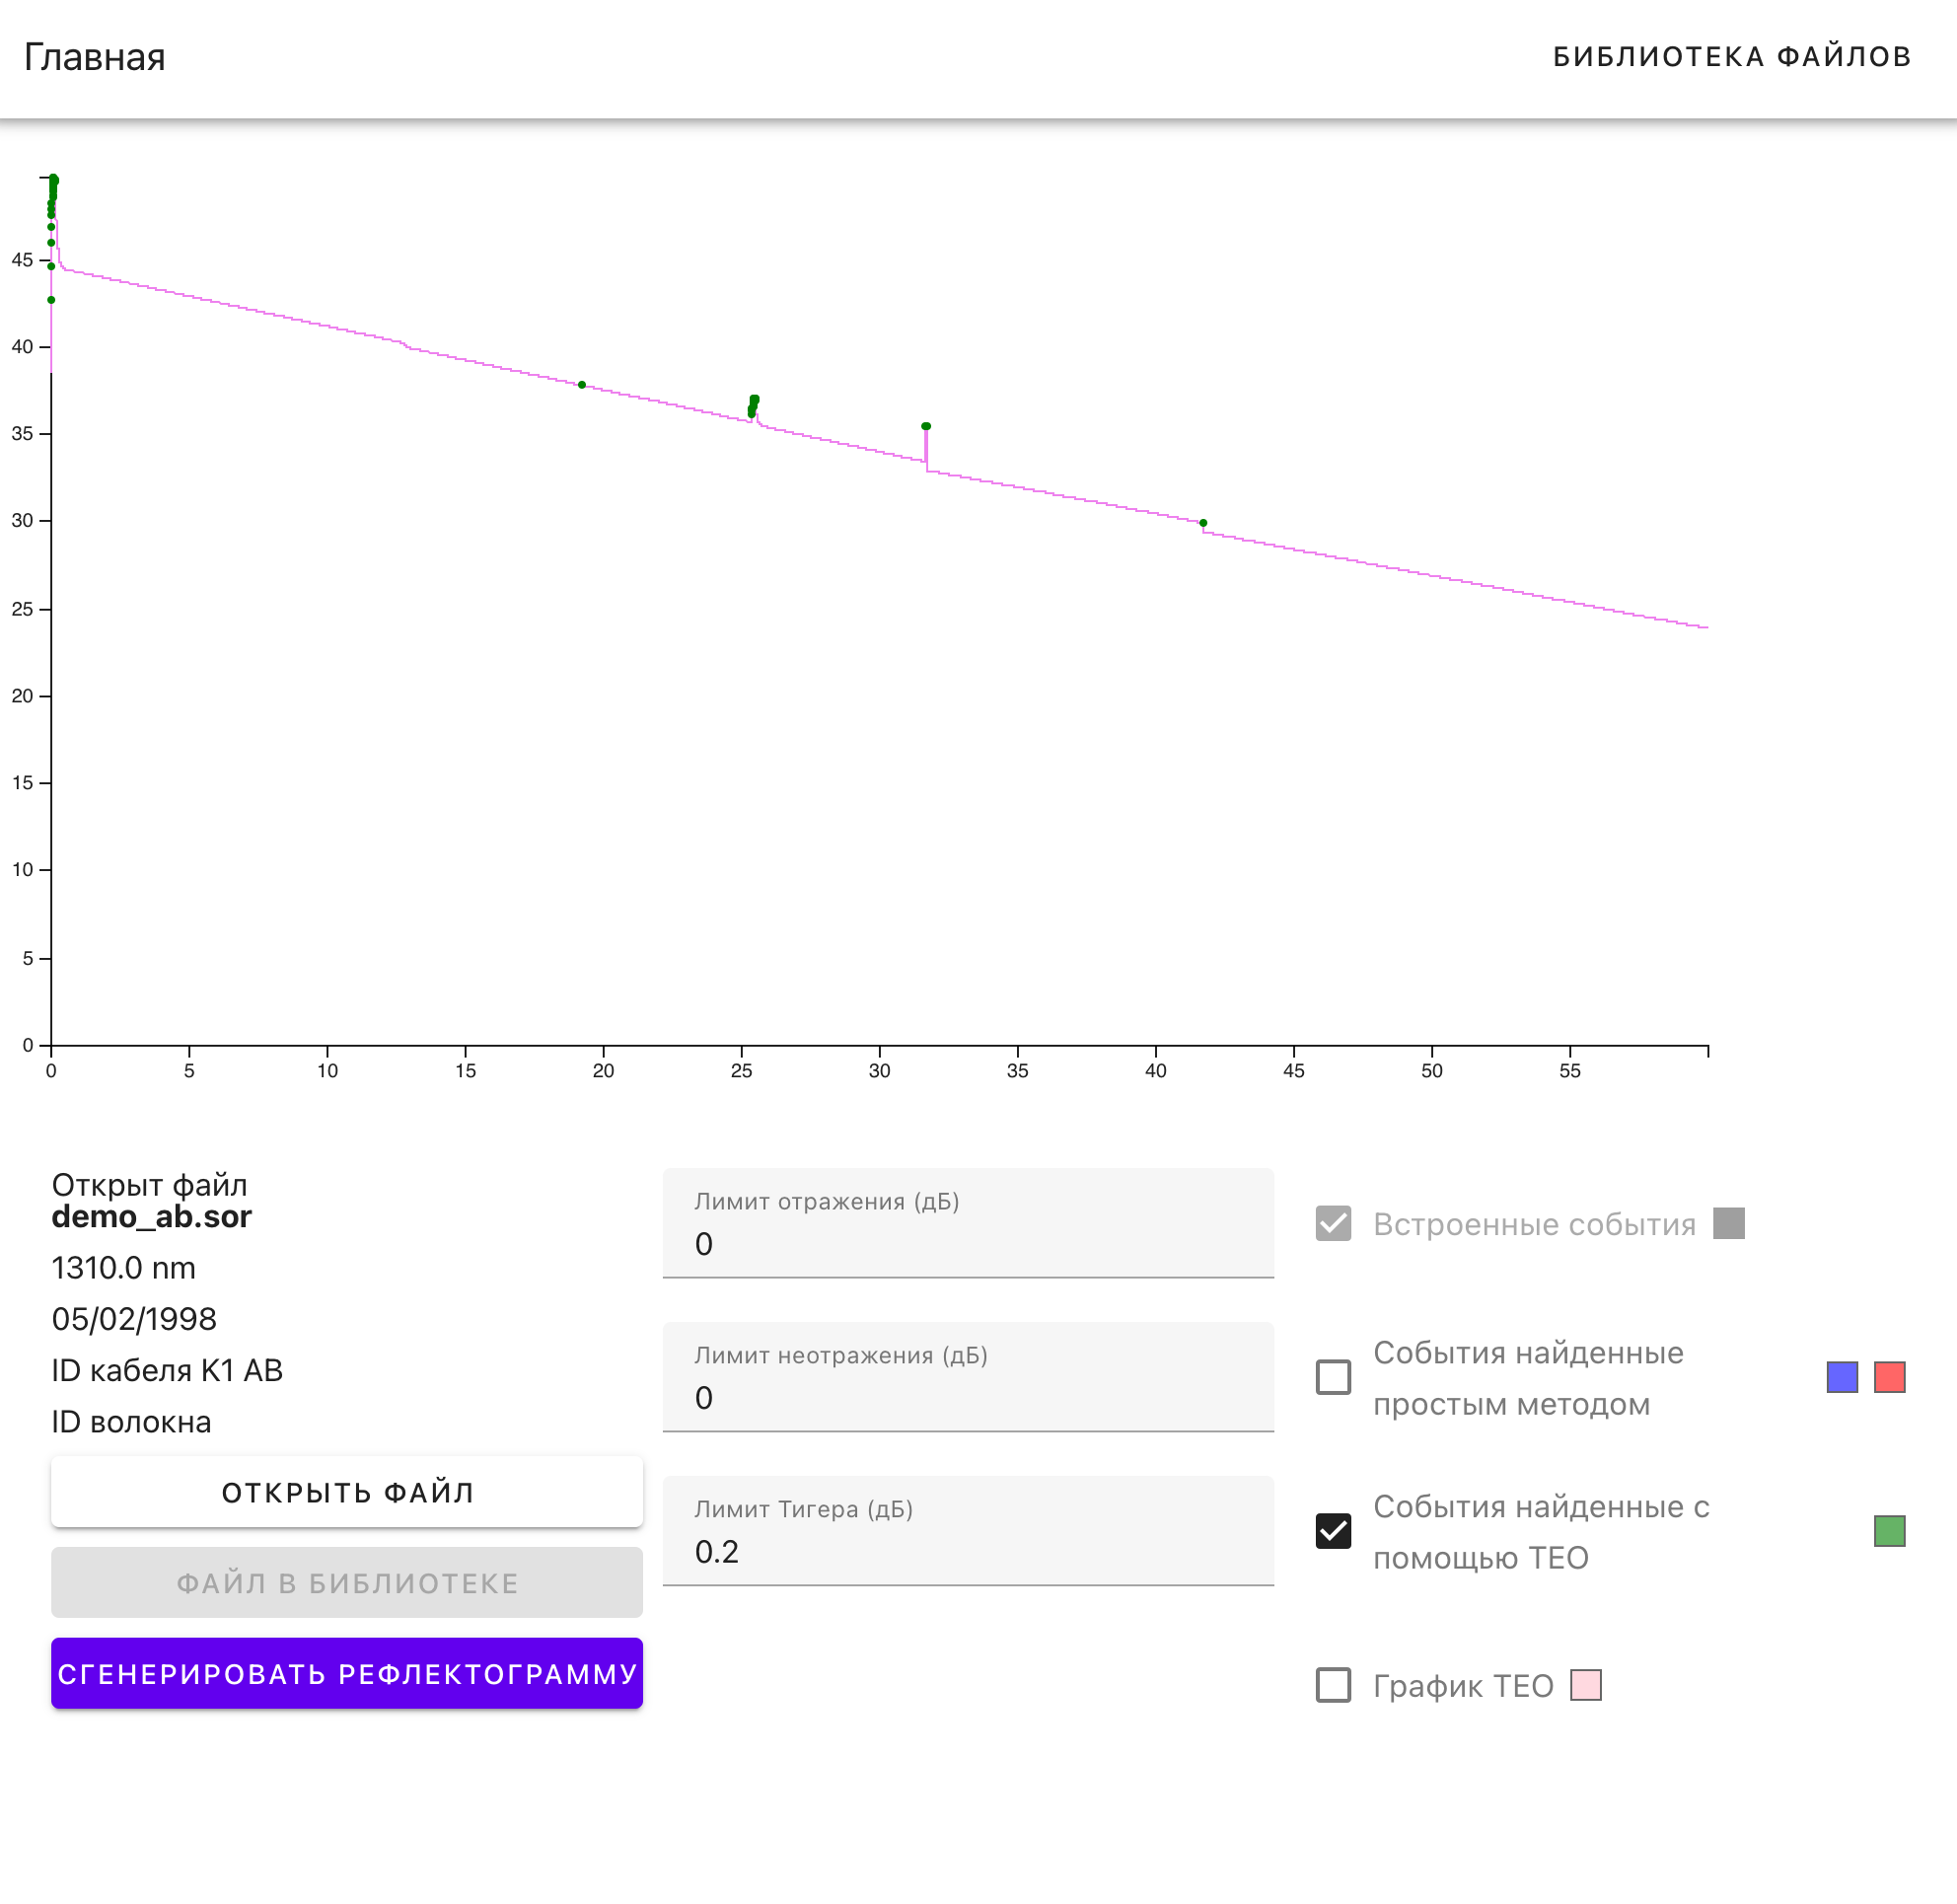
\includegraphics[width=0.65\textwidth]{events_after_editing}}}
  \caption{Поиск событий на отредактированной рефлектограмме}
  \label{ris:events_after_editing}
\end{figure}

\subsection{Выводы по разделу}

В разделе проведен подробный обзор приложения, продемонстрирована работа всех функций приложения.


\newpage
\section*{ЗАКЛЮЧЕНИЕ}
\addcontentsline{toc}{section}{ЗАКЛЮЧЕНИЕ}

Целью работы было создание приложения для хранения и обработки результатов измерения оптических рефлектометров. В ходе работы были подробно рассмотрены выбранные задачи, проведен анализ существующих решений, описаны требования к приложению, после чего разработано и продемонстрировано приложение со следующими характеристиками:

\begin{itemize}
  \item поддержка формата SOR;
  \item отображение событий сохраненных в открытом файле;
  \item поиск и отображение событий с помощью двух алгоритмов;
  \item редактирование рефлектограмм:
  \begin{itemize}
    \item обрезка;
    \item добавление событий;
    \item генерация продолжения рефлектограммы.
  \end{itemize}
  \item сохранение рефлектограмм во встроенную библиотеку;
  \item просмотр и редактирование содержимого библиотеки;
  \item загрузка ранее сохраненных рефлектограмм из встроенной библиотеки;
  \item поддержка операционных систем Windows, Linux, Mac OS.
\end{itemize}

\noindent Среди дальнейших путей развития можно выделить:

\begin{itemize}
  \item добавление возможности просматривать несколько рефлектограмм одновременно;
  \item добавление возможности обрабатывать встречные измерения;
  \item добавление функции экспорта в файл формата SOR;
  \item добавление облачного хранения данных и синхронизации библиотеки между устройствами пользователя.
\end{itemize}

\newpage
\printbibliography[
  heading=bibintoc, 
  title={СПИСОК ИСПОЛЬЗОВАННЫХ ИСТОЧНИКОВ}
]

\newpage
\appendix

\titleformat{\subsection}[display]
  {\normalfont\large\bfseries}
  {\centering Приложение\ \thesubsection}
  {0pt}{\large\centering}

\renewcommand{\thesubsection}{\Asbuk{subsection}}

% \renewcommand\theFancyVerbLine{\footnotesize\arabic{FancyVerbLine}}

\section*{ПРИЛОЖЕНИЯ}
\addcontentsline{toc}{section}{ПРИЛОЖЕНИЯ}

\subsection{Модуль <<main/index.ts>>}
\begin{lstlisting}[language=typescript]
import { app, shell, BrowserWindow, dialog, ipcMain } from "electron";
import { join } from "path";
import fs from "fs";
import { electronApp, optimizer, is } from "@electron-toolkit/utils";
import openSOR from "./openSOR";
import icon from "../../resources/icon.png?asset";
import ElStore from "electron-store";

const elStore = new ElStore({
  defaults: {
    library: [],
  },
});

function createWindow(): void {
  const mainWindow = new BrowserWindow({
    width: 1000,
    height: 1000,
    show: false,
    autoHideMenuBar: true,
    ...(process.platform === "linux" ? { icon } : {}),
    webPreferences: {
      preload: join(__dirname, "../preload/index.js"),
      sandbox: false,
    },
  });

  mainWindow.on("ready-to-show", () => {
    mainWindow.show();
  });

  mainWindow.webContents.setWindowOpenHandler((details) => {
    shell.openExternal(details.url);
    return { action: "deny" };
  });

  if (is.dev && process.env["ELECTRON_RENDERER_URL"]) {
    mainWindow.loadURL(process.env["ELECTRON_RENDERER_URL"]);
  } else {
    mainWindow.loadFile(join(__dirname, "../renderer/index.html"));
  }
}

app.whenReady().then(() => {
  electronApp.setAppUserModelId("com.electron");

  app.on("browser-window-created", (_, window) => {
    optimizer.watchWindowShortcuts(window);
  });

  createWindow();

  app.on("activate", function () {
    if (BrowserWindow.getAllWindows().length === 0) createWindow();
  });

  ipcMain.handle("dialog", (_, method, params) => {
    return dialog[method](BrowserWindow.getAllWindows()[0], params);
  });

  ipcMain.handle("readFile", (_, path: string): string => {
    return fs.readFileSync(path, { encoding: "utf-8" });
  });

  ipcMain.handle("openSOR", (_, path: string) => {
    return openSOR(path);
  });

  ipcMain.on("electron-store-get", async (event, val) => {
    event.returnValue = elStore.get(val);
  });

  ipcMain.on("electron-store-set", async (event, key, val) => {
    elStore.set(key, val);
  });
});

app.on("window-all-closed", () => {
  if (process.platform !== "darwin") {
    app.quit();
  }
});
\end{lstlisting}

\subsection{Модуль <<main/openSOR.ts>>}
\begin{lstlisting}[language=typescript]
import SOR from "jsotdr";
import type TTrace from "../models/trace";
import type TSor from "../models/sor";

const datToTrace = (rows: Array<string>): TTrace => {
  return rows.map((row) => {
    const [x, y] = row.split("\t");
    return {
      x: parseFloat(x),
      y: parseFloat(y),
    };
  });
};

// eslint-disable-next-line
const parseInfo = (raw: any) => {
  return {
    filename: raw.filename,
    Cksum: raw.Cksum,
    KeyEvents: Object.keys(raw.KeyEvents)
      .filter((key) => key !== "Summary" && key !== "num events")
      .map((key) => {
        const event = raw.KeyEvents[key];

        return {
          ...event,
          distance: parseFloat(event.distance),
        };
      }),
    FxdParams: {
      BC: parseFloat(raw.FxdParams["BC"]),
      EOTThr: parseFloat(raw.FxdParams["EOT thr"]),
      date: new Date(raw.FxdParams["date/time"]),
      lossThr: parseFloat(raw.FxdParams["loss thr"]),
      reflThr: parseFloat(raw.FxdParams["refl thr"]),
      pulseWidth: parseFloat(raw.FxdParams["pulse width"]),
      wavelength: raw.FxdParams["wavelength"],
      resolution: raw.FxdParams["resolution"],
    },
    GenParams: {
      cableId: raw.GenParams["cable ID"],
      fiberId: raw.GenParams["fiber ID"],
    },
    Summary: raw.KeyEvents.Summary,
    DataPts: raw.DataPts,
  };
};

export default async (filepath: string): Promise<TSor> => {
  const sor = new SOR();
  const results = await sor.reader(filepath);

  return {
    status: results[0],
    info: parseInfo(results[1]),
    infoRaw: results[1],
    trace: datToTrace(results[2]),
  };
};  
\end{lstlisting}

\subsection{Модуль <<models/coords.ts>>}
\begin{lstlisting}[language=typescript]
type TCoords = {
  x: number;
  y: number;
};

export default TCoords;
\end{lstlisting}

\subsection{Модуль <<models/lineEvent.ts>>}
\begin{lstlisting}[language=typescript]
import TCoords from "./coords";

type TLineEvent = {
  start: TCoords,
  end: TCoords,
  type: "reflection" | "loss",
};

export default TLineEvent;
\end{lstlisting}

\subsection{Модуль <<models/sor.ts>>}
\begin{lstlisting}[language=typescript]
import type TTrace from "./trace";

type TEvent = {
  type: string;
  distance: number;
};

type TSor = {
  status: string;
  infoRaw: unknown;
  info: {
    filename: string;
    FxdParams: {
      BC: number,
      date: Date,
      EOTThr: number,
      lossThr: number,
      reflThr: number,
      pulseWidth: number,
      wavelength: string,
      resolution: number
    },
    GenParams: {
      cableId: string;
      fiberId: string;
    },
    Cksum: {
      checksum: number,
      checksum_ours: number,
      match: boolean
    },
    DataPts: object,
    KeyEvents: TEvent[],
    Summary: object,
  };
  trace: TTrace;
};

export default TSor;  
\end{lstlisting}
\subsection{Модуль <<models/trace.ts>>}
\begin{lstlisting}[language=typescript]
import type TCoords from "./coords";

type TTrace = TCoords[];

export default TTrace;
\end{lstlisting}
\subsection{Модуль <<preload/index.d.ts>>}
\begin{lstlisting}[language=typescript]
import { ElectronAPI } from "@electron-toolkit/preload";

declare global {
  interface Window {
    electron: ElectronAPI & {
      store: {
        get: (key: string) => any;
        set: (key: string, val: any) => void;
      }
    }
    electron: ElectronAPI
    api: unknown
  }
}  
\end{lstlisting}

\subsection{Модуль <<preload/index.ts>>}
\begin{lstlisting}[language=typescript]
import { contextBridge, ipcRenderer } from "electron";
import { electronAPI } from "@electron-toolkit/preload";

const api = {};

if (process.contextIsolated) {
  try {
    contextBridge.exposeInMainWorld("electron", {
      ...electronAPI,
      store: {
        get(key) {
          return ipcRenderer.sendSync("electron-store-get", key);
        },
        set(property, val) {
          ipcRenderer.send("electron-store-set", property, val);
        },
      },
    });
    contextBridge.exposeInMainWorld("api", api);
  } catch (error) {
    console.error(error);
  }
} else {
  // @ts-ignore (define in dts)
  window.electron = electronAPI;
  // @ts-ignore (define in dts)
  window.api = api;
}
\end{lstlisting}

\subsection{Модуль <<renderer/src/assets/css/base.scss>>}
\begin{lstlisting}[language=scss]
@import 'reset-css';

body {
  font-family: Roboto, -apple-system, BlinkMacSystemFont, 'Helvetica Neue', 'Segoe UI', 'Oxygen',
    'Ubuntu', 'Cantarell', 'Open Sans', sans-serif;
}
\end{lstlisting}

\subsection{Модуль <<renderer/src/views/Home/Index.vue>>}
\begin{lstlisting}[language=vue]
<script setup lang="ts">
import { ref, computed, toRaw } from "vue";
import TraceChart from "./TraceChart.vue";
import GenerateModal from "./GenerateModal.vue";
import ActionsModal from "./ActionsModal.vue";
import type TSor from "src/models/sor";
import { useStore } from "@renderer/store";
import { storeToRefs } from "pinia";

const store = useStore();
const { sor } = storeToRefs(store);

const lossThr = ref<string>();
const reflThr = ref<string>();
const teoThr = ref<string>("0.2");

const showBuiltin = ref<boolean>(true);
const showNaive = ref<boolean>(false);
const showTeo = ref<boolean>(true);
const showTeoVal = ref<boolean>(false);

const sorEdited = ref(false);
const justSavedToLib = ref<boolean>(false);
const showActionsModal = ref();
const clickX = ref<number>();

const openFile = async (): Promise<void> => {
  const dialogConfig = {
    properties: ["openFile"],
  };

  const result = await window.electron.ipcRenderer.invoke("dialog", "showOpenDialog", dialogConfig);
  const filePath = result.filePaths[0];

  sor.value = await window.electron.ipcRenderer.invoke("openSOR", filePath) as TSor;
  lossThr.value = String(sor.value.info.FxdParams.lossThr);
  reflThr.value = String(sor.value.info.FxdParams.reflThr);
  justSavedToLib.value = false;
  sorEdited.value = false;

  console.log(sor.value);
};

const inLibrary = computed((): boolean => {
  if (!sor.value) {
    return false;
  }

  if (justSavedToLib.value) {
    return true;
  }

  const library = window.electron.store.get("library");
  return library.some((s) => s.info.filename === sor.value?.info.filename);
});

const saveToLibrary = (): void => {
  if (!sor.value) {
    return;
  }

  justSavedToLib.value = true;
  const library = window.electron.store.get("library");
  library.push(toRaw(sor.value));
  window.electron.store.set("library", library);
};

const updateLoss = (value: string): void => {
  if (!sor.value) {
    return;
  }

  sor.value.info.FxdParams.lossThr = parseFloat(value);
};

const updateRefl = (value: string): void => {
  if (!sor.value) {
    return;
  }

  sor.value.info.FxdParams.reflThr = parseFloat(value);
};

function crop(x: number): void {
  if (!sor.value) {
    return;
  }

  sor.value.trace = sor.value.trace.filter((dp) => dp.x < x);
  sorEdited.value = true;
}

function generate({
  att, noiseScale,
}: { att: number, noiseScale: number }): void {
  if (!sor.value) {
    return;
  }

  while(sor.value.trace.length < sor.value.info.DataPts["num data points"]) {
    const lastDP = sor.value.trace[sor.value.trace.length - 1];

    const step = sor.value.info.FxdParams.resolution * 0.001;

    const stepAtt = att * step;
    const noise = noiseScale * (Math.random() - .5) * stepAtt;

    // Potentially causing excessive rerenderings
    sor.value.trace.push({
      x: lastDP.x + step,
      y: lastDP.y - stepAtt + noise,
    });
  }
}

function addEvent({
  x,
  type,
  loss,
  reflection,
}: {
  x: number,
  type: "reflection" | "loss",
  loss: number,
  reflection: number
}): void {
  if (!sor.value) {
    return;
  }

  const length = 8;

  const eventStart = sor.value.trace.findIndex((dp) => dp.x > x);
  const eventEnd = eventStart + length;

  for (let i = eventStart; i < eventEnd; i++) {
    if (type === "loss") {
      sor.value.trace[i].y = sor.value.trace[i].y - loss;
    } else {
      sor.value.trace[i].y = sor.value.trace[i].y + reflection;
    }
  }

  for (let i = eventEnd; i <= sor.value.trace.length; i++) {
    sor.value.trace[i].y = sor.value.trace[i].y - loss;
  }
}

function handleClickTrace(x: number): void {
  showActionsModal.value = true;
  clickX.value = x;
}
</script>

<template>
  <v-app-bar title="Главная">
    <template #append>
      <v-btn @click="store.navigate('library')">
        Библиотека файлов
      </v-btn>
    </template>
  </v-app-bar>

  <v-main>
    <TraceChart
      v-if="sor"
      :sor="sor"
      :teo-thr="parseFloat(teoThr)"
      :show-builtin="showBuiltin"
      :show-naive="showNaive"
      :show-teo="showTeo"
      :show-teo-val="showTeoVal"
      :sor-edited="sorEdited"
      @click-trace="handleClickTrace"
    />

    <div
      v-if="sor"
      class="controls"
    >
      <div class="controls__file">
        <div>
          Открыт файл
          <b class="controls__file__filename">{{ sor.info.filename }}</b>
        </div>
        <div>
          {{ sor.info.FxdParams.wavelength }}
        </div>
        <div>
          {{ new Intl.DateTimeFormat('ru-RU').format(new Date(sor.info.FxdParams.date)) }}
        </div>
        <div>
          ID кабеля {{ sor.info.GenParams.cableId }}
        </div>
        <div>
          ID волокна {{ sor.info.GenParams.fiberId }}
        </div>
        <v-btn
          class="controls__file__open"
          @click="openFile"
        >
          Открыть файл
        </v-btn>
        <v-btn
          v-if="!inLibrary"
          class="controls__file__save"
          @click="saveToLibrary"
        >
          Сохранить файл в библиотеку
        </v-btn>
        <v-btn
          v-else
          class="controls__file__save"
          disabled
        >
          Файл в библиотеке
        </v-btn>

        <GenerateModal
          @generate="generate"
        />
        <ActionsModal
          v-model="showActionsModal"
          :click-x="(clickX as number)"
          @add-event="addEvent"
          @crop="crop"
        />
      </div>
      <div
        v-if="sor"
        class="controls__settings"
      >
        <div class="controls__settings__naive">
          <v-text-field
            v-model="reflThr"
            label="Лимит отражения (дБ)"
            @update:model-value="updateRefl"
          />
          <v-text-field
            v-model="lossThr"
            label="Лимит неотражения (дБ)"
            @update:model-value="updateLoss"
          />
          <v-text-field
            v-model="teoThr"
            label="Лимит Тигера (дБ)"
          />
        </div>
        <div class="controls__settings__teo">
          <v-checkbox
            v-model="showBuiltin"
            :disabled="sorEdited"
          >
            <template #label>
              Встроенные события
              <div
                class="colorIndicator"
                style="background: black;"
              ></div>
            </template>
          </v-checkbox>
          <v-checkbox
            v-model="showNaive"
          >
            <template #label>
              События найденные простым методом
              <div
                class="colorIndicator"
                style="background: blue;"
              ></div>
              <div
                class="colorIndicator"
                style="background: red;"
              ></div>
            </template>
          </v-checkbox>
          <v-checkbox
            v-model="showTeo"
          >
            <template #label>
              События найденные с помощью TEO
              <div
                class="colorIndicator"
                style="background: green;"
              ></div>
            </template>
          </v-checkbox>
          <v-checkbox
            v-model="showTeoVal"
          >
            <template #label>
              График TEO
              <div
                class="colorIndicator"
                style="background: pink;"
              ></div>
            </template>
          </v-checkbox>
        </div>
      </div>
    </div>
    <v-btn
      v-else
      class="openFile"
      color="primary"
      @click="openFile"
    >
      Открыть файл
    </v-btn>
  </v-main>
</template>

<style scoped lang="scss">
.openFile {
  top: 50%;
  left: 50%;
  transform: translate(-50%, -50%);
}

.controls {
  padding: 30px;
  display: flex;
  gap: 10px;
}

.controls__file,
.controls__settings {
  display: flex;
}

.controls__file {
  gap: 10px;
  width: 300px;
  flex-direction: column;
}

.controls__file__filename {
  display: block;
  overflow: hidden;
  text-overflow: ellipsis;
}

.controls__settings {
  flex-direction: row;
  flex-grow: 1;
  flex-wrap: wrap;
  gap: 10px;

  > * {
    flex-grow: 1;
    box-sizing: border-box;
    width: calc(50% - 10px);
  }
}

.colorIndicator {
  width: 16px;
  min-width: 16px;
  height: 16px;
  border: 1px solid black;
  margin-left: 8px;
}
</style>  
\end{lstlisting}

\subsection{Модуль <<renderer/src/views/Home/ActionsModal.vue>>}
\begin{lstlisting}[language=vue]
<template>
  <v-dialog
    v-model="show"
    width="auto"
  >
    <v-card class="card">
      <v-switch
        v-model="isReflective"
        :label="isReflective ? '%*отражающее событие*)' : '%*неотражающее событие*)'"
      />
      <v-text-field
        v-model="loss"
        label="%*Потери (дБ)*)"
      />
      <v-text-field
        v-model="reflection"
        label="%*Отражение (дБ)*)"
      />

      <v-card-actions class="actions">
        <v-btn
          @click="show = false"
        >
          Закрыть
        </v-btn>
        <v-btn
          @click="crop"
        >
          <v-icon>
            mdi-content-cut
          </v-icon>
        </v-btn>
        <v-btn
          @click="addEvent"
        >
          Добавить событие
        </v-btn>
      </v-card-actions>
    </v-card>
  </v-dialog>
</template>

<script setup lang="ts">
import { computed, ref } from "vue";

const isReflective = ref(false);
const loss = ref(.5);
const reflection = ref(2);

const props = defineProps<{
  modelValue: boolean;
  clickX: number;
}>();

const emit = defineEmits<{
  (event: "update:modelValue", value: boolean): void;
  (event: "addEvent", value: {
    x: number,
    type: "reflection" | "loss",
    loss: number,
    reflection: number,
  }): void;
  (event: "crop", value: number): void;
}>();

const show = computed({
  get() {
    return props.modelValue;
  },
  set(value) {
    emit("update:modelValue", value);
  },
});

function crop(): void {
  emit("crop", props.clickX);
  show.value = false;
}

function addEvent(): void {
  show.value = false;
  emit("addEvent", {
    x: props.clickX,
    type: isReflective.value ? "reflection" : "loss",
    loss: loss.value,
    reflection: reflection.value,
  });
}
</script>

<style scoped lang="scss">
.card {
  padding: 25px;
}

.actions {
  display: flex;
  justify-content: space-evenly;
}
</style>
\end{lstlisting}

\subsection{Модуль <<renderer/src/views/Home/GenerateModal.vue>>}
\begin{lstlisting}[language=vue]
<script setup lang="ts">
import { ref } from "vue";

const emit = defineEmits<{
  (event: "generate", value: {
    att: number,
    noiseScale: number
  }): void
}>();

const dialog = ref();

const att = ref(0.25);
const noiseScale = ref(2);
</script>

<template>
  <v-dialog
    v-model="dialog"
    width="auto"
  >
    <template #activator="{ props }">
      <v-btn
        color="primary"
        v-bind="props"
      >
        Сгенерировать рефлектограмму
      </v-btn>
    </template>

    <v-card class="card">
      <v-text-field
        v-model="att"
        label="%*Затухание (дБ/км)*)"
      />
      <v-text-field
        v-model="noiseScale"
        label="%*Масштаб шума*)"
      />

      <v-card-actions class="actions">
        <v-btn
          @click="dialog = false"
        >
          Закрыть
        </v-btn>

        <v-btn
          color="primary"
          @click="() => {
            dialog = false
            emit('generate', { att, noiseScale })
          }"
        >
          Сгенерировать рефлектограмму
        </v-btn>
      </v-card-actions>
    </v-card>
  </v-dialog>
</template>

<style scoped lang="scss">
.card {
  padding: 25px;
}

.actions {
  display: flex;
  justify-content: space-evenly;
}
</style>  
\end{lstlisting}

\subsection{Модуль <<renderer/src/views/Home/TraceChart.vue>>}
\begin{lstlisting}[language=vue]
<script setup lang="ts">
import { watch, onMounted, ref } from "vue";
import * as d3 from "d3";
import type TSor from "src/models/sor";
import type TTrace from "src/models/trace";
import type TCoords from "src/models/coords";
import type TLineEvent from "src/models/lineEvent";

const props = defineProps<{
  sor: TSor;
  teoThr: number;
  showBuiltin: boolean;
  showNaive: boolean;
  showTeo: boolean;
  showTeoVal: boolean;
  sorEdited: boolean;
}>();

const emit = defineEmits<{
(event: "clickTrace", value: number): void;
}>();

const foundEvents = ref<TLineEvent[]>([]);
const teoValues = ref<(TCoords & { tX: number, tY: number })[]>([]);
const teoEvents = ref<TLineEvent[]>([]);

const padding = {
  top: 30,
  bottom: 30,
  left: 30,
  right: 30,
};
const width = 900 - padding.left - padding.right;
const height = 500 - padding.top - padding.bottom;

const x = d3
  .scaleLinear()
  .domain(
    d3.extent(
      props.sor.trace,
      (d) => d.x,
    ) as Iterable<d3.NumberValue>,
  )
  .rangeRound([0, width]);

const y = d3
  .scaleLinear()
  .domain(
    d3.extent(
      props.sor.trace,
      (d) => d.y,
    ) as Iterable<d3.NumberValue>,
  )
  .rangeRound([height, 0]);

const drawChart = (): void => {
  const svg = d3.select("#trace")
    .attr("width", width + padding.left + padding.right)
    .attr("height", height + padding.top + padding.bottom);

  svg.selectAll("g").remove();

  const g = svg.append("g")
    .attr("transform", `translate(${padding.left}, ${padding.top})`);

  const line = d3.line<TTrace[number]>()
    .x((d) => x(d.x))
    .y((d) => y(d.y));

  g.append("g")
    .attr("transform", `translate(0, ${height})`)
    .call(d3.axisBottom(x));

  g.append("g")
    .call(d3.axisLeft(y));

  g.append("path")
    .datum(props.sor.trace)
    .attr("fill", "none")
    .attr("stroke", "violet")
    .attr("stroke-width", 1)
    .attr("d", line);

  // Draw included in file events
  if (props.showBuiltin && !props.sorEdited) {
    const includedEvents: { x: number; y: number | null }[] = props.sor.info.KeyEvents.map((e) => ({ x: e.distance, y: null }));
    props.sor.trace.forEach((dp) => {
      includedEvents.forEach((event) => {
        if (event.x >= dp.x) {
          event.y = dp.y;
        }
      });
    });

    g.selectAll(".included")
      .data(includedEvents as TTrace)
      .enter()
      .append("circle")
      .attr("class", "included")
      .attr("r", 2)
      .attr("cx", (d) => x(d.x))
      .attr("cy", (d) => y(d.y));
  }

  // Draw naively found events
  if (props.showNaive) {
    g.selectAll(".found")
      .data(foundEvents.value)
      .enter()
      .append("circle")
      .attr("class", "found")
      .attr("fill", (d) => d.type === "loss" ? "red" : "blue")
      .attr("r", 2)
      .attr("cx", (d) => x(d.start.x))
      .attr("cy", (d) => y(d.start.y));
  }

  // Draw teo found events
  if (props.showTeo) {
    g.selectAll(".teo")
      .data(teoEvents.value)
      .enter()
      .append("circle")
      .attr("class", "teo")
      .attr("fill", "green")
      .attr("r", 2)
      .attr("cx", (d) => x(d.start.x))
      .attr("cy", (d) => y(d.start.y));
  }

  if (props.showTeoVal) {
    const teoLine = d3.line<TCoords & { tX: number, tY: number }>()
      .x((d) => x(d.tX))
      .y((d) => y(d.tY));

    g.append("path")
      .datum(teoValues.value)
      .attr("fill", "none")
      .attr("stroke", "pink")
      .attr("stroke-width", 1)
      .attr("d", teoLine);
  }
};

watch(
  props,
  () => {
    drawChart();
  },
  { deep: true },
);

watch(
  () => props,
  () => {
    foundEvents.value = ((): TLineEvent[] => {
      const clumps: TLineEvent[] = [];
      let currentClump: {
        start: TCoords,
        end?: TCoords,
        type: "reflection" | "loss",
      } | null = null;

      props.sor.trace.forEach((dp, i) => {
        if (i === 0) {
          return;
        }

        if (!currentClump) {
          if (dp.y - props.sor.trace[i - 1].y > -props.sor.info.FxdParams.reflThr) {
            currentClump = {
              start: props.sor.trace[i - 1],
              type: "reflection",
            };
          }

          if (dp.y - props.sor.trace[i - 1].y < -props.sor.info.FxdParams.lossThr) {
            currentClump = {
              start: dp,
              type: "loss",
            };
          }
        } else {
          if (dp.y <= currentClump.start.y) {
            currentClump.end = dp;
            clumps.push(currentClump as TLineEvent);
            currentClump = null;
          }
        }
      });

      return clumps;
    })();

    teoValues.value = ((): (TCoords & { tX: number, tY: number })[] => {
      const teo: (TCoords & { tX: number, tY: number })[] = [];
      props.sor.trace.forEach((dp, i) => {
        if (i === 0 || i === props.sor.trace.length - 1) {
          return;
        }

        const prev = props.sor.trace[i - 1];
        const next = props.sor.trace[i + 1];

        teo.push({
          tX: dp.x,
          tY: dp.y * dp.y - (prev.y * next.y),
          x: dp.x,
          y: dp.y,
        });
      });

      return teo;
    })();

    teoEvents.value = ((): TLineEvent[] => {
      const result: TLineEvent[] = [];
      teoValues.value.forEach((dp) => {
        if (dp.tY >= props.teoThr) {
          result.push({
            start: dp,
            end: dp,
            type: "loss",
          });
        }
      });

      return result;
    })();

    drawChart();
  },
  { deep: true, immediate: true },
);

onMounted(() => {
  drawChart();
});

function clickTrace(event: MouseEvent): void {
  const clickX = x.invert(event.clientX - padding.left);
  emit("clickTrace", clickX);
}
</script>

<template>
  <svg
    id="trace"
    @click="clickTrace"
  ></svg>
</template>

<style scoped>
#trace {
  height: 500px;
}
</style>  
\end{lstlisting}

\subsection{Модуль <<renderer/src/views/Library/Index.vue>>}
\begin{lstlisting}[language=vue]
<script setup lang="ts">
import { useStore } from "@renderer/store";
import type TSor from "src/models/sor";

const store = useStore();

const library = window.electron.store.get("library");

function open(sor: TSor): void {
  store.sor = sor;
  store.view = "home";
}

function deleteFromLib(sor: TSor): void {
  const library = window.electron.store.get("library");
  window.electron.store.set("library", library.filter((s) => s.info.filename !== sor.info.filename));
}
</script>

<template>
  <v-app-bar title="Библиотека файлов">
    <template #append>
    </template>
  </v-app-bar>

  <v-main>
    <v-list>
      <template
        v-for="(sor, index) in library"
        :key="sor.info.filename"
      >
        <v-hover
          v-slot="{ isHovering, props }"
        >
          <v-list-item
            v-bind="props"
            class="library__item"
            :class="{
              'bg-grey-darken-1': isHovering
            }"
            :title="sor.info.filename"
            lines="three"
            @click="open(sor)"
          >
            <template #subtitle>
              <div>{{ sor.info.FxdParams.date }}</div>
              <div class="library__item__lineInfo">
                <span>{{ sor.infoRaw.GenParams["cable ID"] }}</span>
                <span>{{ sor.infoRaw.GenParams["fiber ID"] }}</span>
                <span>{{ sor.info.FxdParams.wavelength }}</span>
              </div>
              <div>{{ sor.infoRaw.GenParams["comments"] }}</div>
            </template>
            <template #append>
              <v-icon
                class="library__item__close"
                @click="deleteFromLib(sor)"
              >
                mdi-close
              </v-icon>
            </template>
          </v-list-item>
        </v-hover>

        <v-divider
          v-if="index + 1 < library.length"
          :key="index"
        ></v-divider>
      </template>
    </v-list>
  </v-main>
</template>

<style scoped lang="scss">
.library__item {
  cursor: pointer;
}

.library__item__lineInfo {
  display: flex;
  gap: 8px;
}

.library__item__close {
  z-index: 20;
}
</style>  
\end{lstlisting}

\subsection{Модуль <<renderer/src/App.vue>>}
\begin{lstlisting}[language=vue]
<script setup lang="ts">
import Home from "./views/Home/Index.vue";
import Library from "./views/Library/Index.vue";

import { useStore } from "./store";

const store = useStore();

const views = {
  home: Home,
  library: Library,
};
</script>

<template>
  <v-app>
    <component
      :is="views[store.view]"
    />
  </v-app>
</template>
\end{lstlisting}
\subsection{Модуль <<renderer/src/env.d.ts>>}
\begin{lstlisting}[language=typescript]
/// <reference types="vite/client" />

declare module "*.vue" {
  import type { DefineComponent } from "vue";
  // eslint-disable-next-line @typescript-eslint/no-explicit-any, @typescript-eslint/ban-types
  const component: DefineComponent<{}, {}, any>;
  export default component;
}  
\end{lstlisting}

\subsection{Модуль <<renderer/src/main.ts>>}
\begin{lstlisting}[language=typescript]
import { createApp } from "vue";
import App from "./App.vue";
import { createPinia } from "pinia";
import "./assets/css/base.scss";
import "vuetify/styles";
import { createVuetify } from "vuetify";
import "@mdi/font/css/materialdesignicons.css";
import { mdi, aliases } from "vuetify/iconsets/mdi";
import * as components from "vuetify/components";
import * as directives from "vuetify/directives";

const vuetify = createVuetify({
  components,
  directives,
  icons: {
    defaultSet: "mdi",
    aliases,
    sets: {
      mdi,
    },
  },
});
const pinia = createPinia();

const app = createApp(App);
app.use(pinia);
app.use(vuetify);
app.mount("#app");  
\end{lstlisting}

\subsection{Модуль <<renderer/src/store.ts>>}
\begin{lstlisting}[language=typescript]
import type TSor from "src/models/sor";
import { defineStore } from "pinia";

export const useStore = defineStore("store", {
  state: (): {
    view: "home" | "library",
    sor: TSor | null,
  } => ({
    view: "home",
    sor: null,
  }),
  actions: {
    navigate(view: "home" | "library") {
      this.view = view;
    },
  },
});  
\end{lstlisting}

\subsection{Модуль <<renderer/index.html>>}
\begin{lstlisting}[language=HTML]
<!DOCTYPE html>
<html>
  <head>
    <meta charset="UTF-8" />
    <title>Программа для хранения и обработки результатов измерения оптических рефлектометров</title>
    <!-- https://developer.mozilla.org/en-US/docs/Web/HTTP/CSP -->
    <meta
      http-equiv="Content-Security-Policy"
      content="default-src 'self'; script-src 'self'; style-src 'self' 'unsafe-inline'"
    />
  </head>

  <body>
    <div id="app"></div>
    <script type="module" src="/src/main.ts"></script>
  </body>
</html>  
\end{lstlisting}



\end{document}
